\chapter{Risultati}
\label{cha:risultati}

Questa sezione conclude il lavoro della tesi attraverso la presentazione dei risultati ottenuti e una discussione sul loro possibile significato. Inizieremo con una serie di osservazioni che abbiamo effettuato subito dopo il salvataggio delle immagini, passando poi all'analisi dei dati ricavati dal calcolo del \textit{Mean Square Error} e del \textit{Peak Signal-to-Noise Ratio} (\ref{sec:mse_psnr_results}). Successivamente commenteremo i risultati della visualizzazione Isomap (\ref{sec:feaure_results}) e in chiusura, grazie alle \textit{confusion matrix}, trarremo le conclusioni sulla fase di classificazione (\ref{sec:classification_results}).\\

Le immagini ottenute dalla condivisione riportano significative differenze per quanto riguarda la risoluzione e le dimensioni dei file. I metodi utilizzati per l'upload modificano questi parametri per ridurre lo spazio occupato, ma solo in alcune circostanze. Le immagini con risoluzione $1012\times1800$ e $1687\times3000$ sono state ridimensionate a $899\times1600$ mentre quelle con risoluzione $337\times600$ non sono state alterate. Nell'insieme dei dati ottenuti abbiamo osservato due casi particolari: \textit{IPHONE} e \textit{ANDROID}. Nel primo le immagini “medie" e “grandi" sono state ridotte a $576\times1024$, nel secondo solo quelle $1687\times3000$ hanno subito variazioni con una risoluzione finale di $1151\times2048$ pixel. Per tutte le immagini l'\textit{aspect ratio} è rimasto invariato a $9:16$. Questi risultati ci hanno fatto capire che WhatsApp comprime i file solamente se la loro risoluzione supera una determinata soglia. Per quanto riguarda invece la dimensione, essendo direttamente proporzionale alla risoluzione delle immagini essa è cambiata di conseguenza.

\section{MSE - PSNR}
\label{sec:mse_psnr_results}
I \textit{boxplot} in Fig.~\ref{fig:mse_results} mostrano i valori del \textit{Mean Square Error} ottenuti confrontando le immagini di SHADE per ogni coppia di metodi di condivisione. Dai dati a nostra disposizione possiamo formulare le seguenti considerazioni:

\begin{enumerate}
    \item Le immagini condivise tramite l'applicazione desktop per MacOS e Windows 10 (rispettivamente \textit{APP-MAC} e \textit{APP-WIN}) risultano simili tra di loro dato il limitato intervallo di numeri. Analizzando le coppie (\textit{APP-MAC, WEB-WIN}) e (\textit{APP-WIN, WEB-WIN}) confermiamo quanto appena detto poiché le immagini caricate tramite le applicazioni desktop e Chrome presentano valori molto simili. Tale elemento suggerisce che \textit{APP-MAC} e \textit{APP-WIN} hanno somiglianze dal punto di vista implementativo.
    
    \item Anche le immagini condivise tramite Safari (\textit{WEB-MAC, WEB-IPAD}) sono similari, con il \textit{Mean Square Error} che non va oltre $1.2$. Confrontando questi risultati con quelli delle coppie (\textit{WEB-MAC}, \textit{APP-WIN}) e (\textit{WEB-IPAD}, \textit{APP-WIN}) possiamo supporre che le operazioni svolte dallo stesso browser ma su dispositivi differenti siano le medesime.
    
    \item Sia per le coppie (\textit{APP-MAC}, \textit{WEB-MAC}) e (\textit{APP-MAC}, \textit{WEB-IPAD}) si evidenziano differenze tra le immagini nonostante siano state condivise tramite dispositivi appartenenti allo stesso brand (Apple). Ciò dimostra le diverse scelte per le regole di upload anche se i sistemi operativi su cui vengono svolte le operazioni sono simili.
    
    \item Non tutte le coppie di immagini sono presenti in questi risultati a causa della diversa risoluzione degli elementi analizzati. Infatti, le classi \textit{ANDROID} e \textit{IPHONE} sono state escluse perché non potevano essere confrontate con le altre.
    
    \item Tutte le immagini aventi risoluzione $337\times600$ hanno ottenuto valori del MSE pari a 0 dimostrando come, qualitativamente, le piattaforme di condivisione non abbiano modificato in alcun modo questi file.
\end{enumerate}

\begingroup
    \centering
    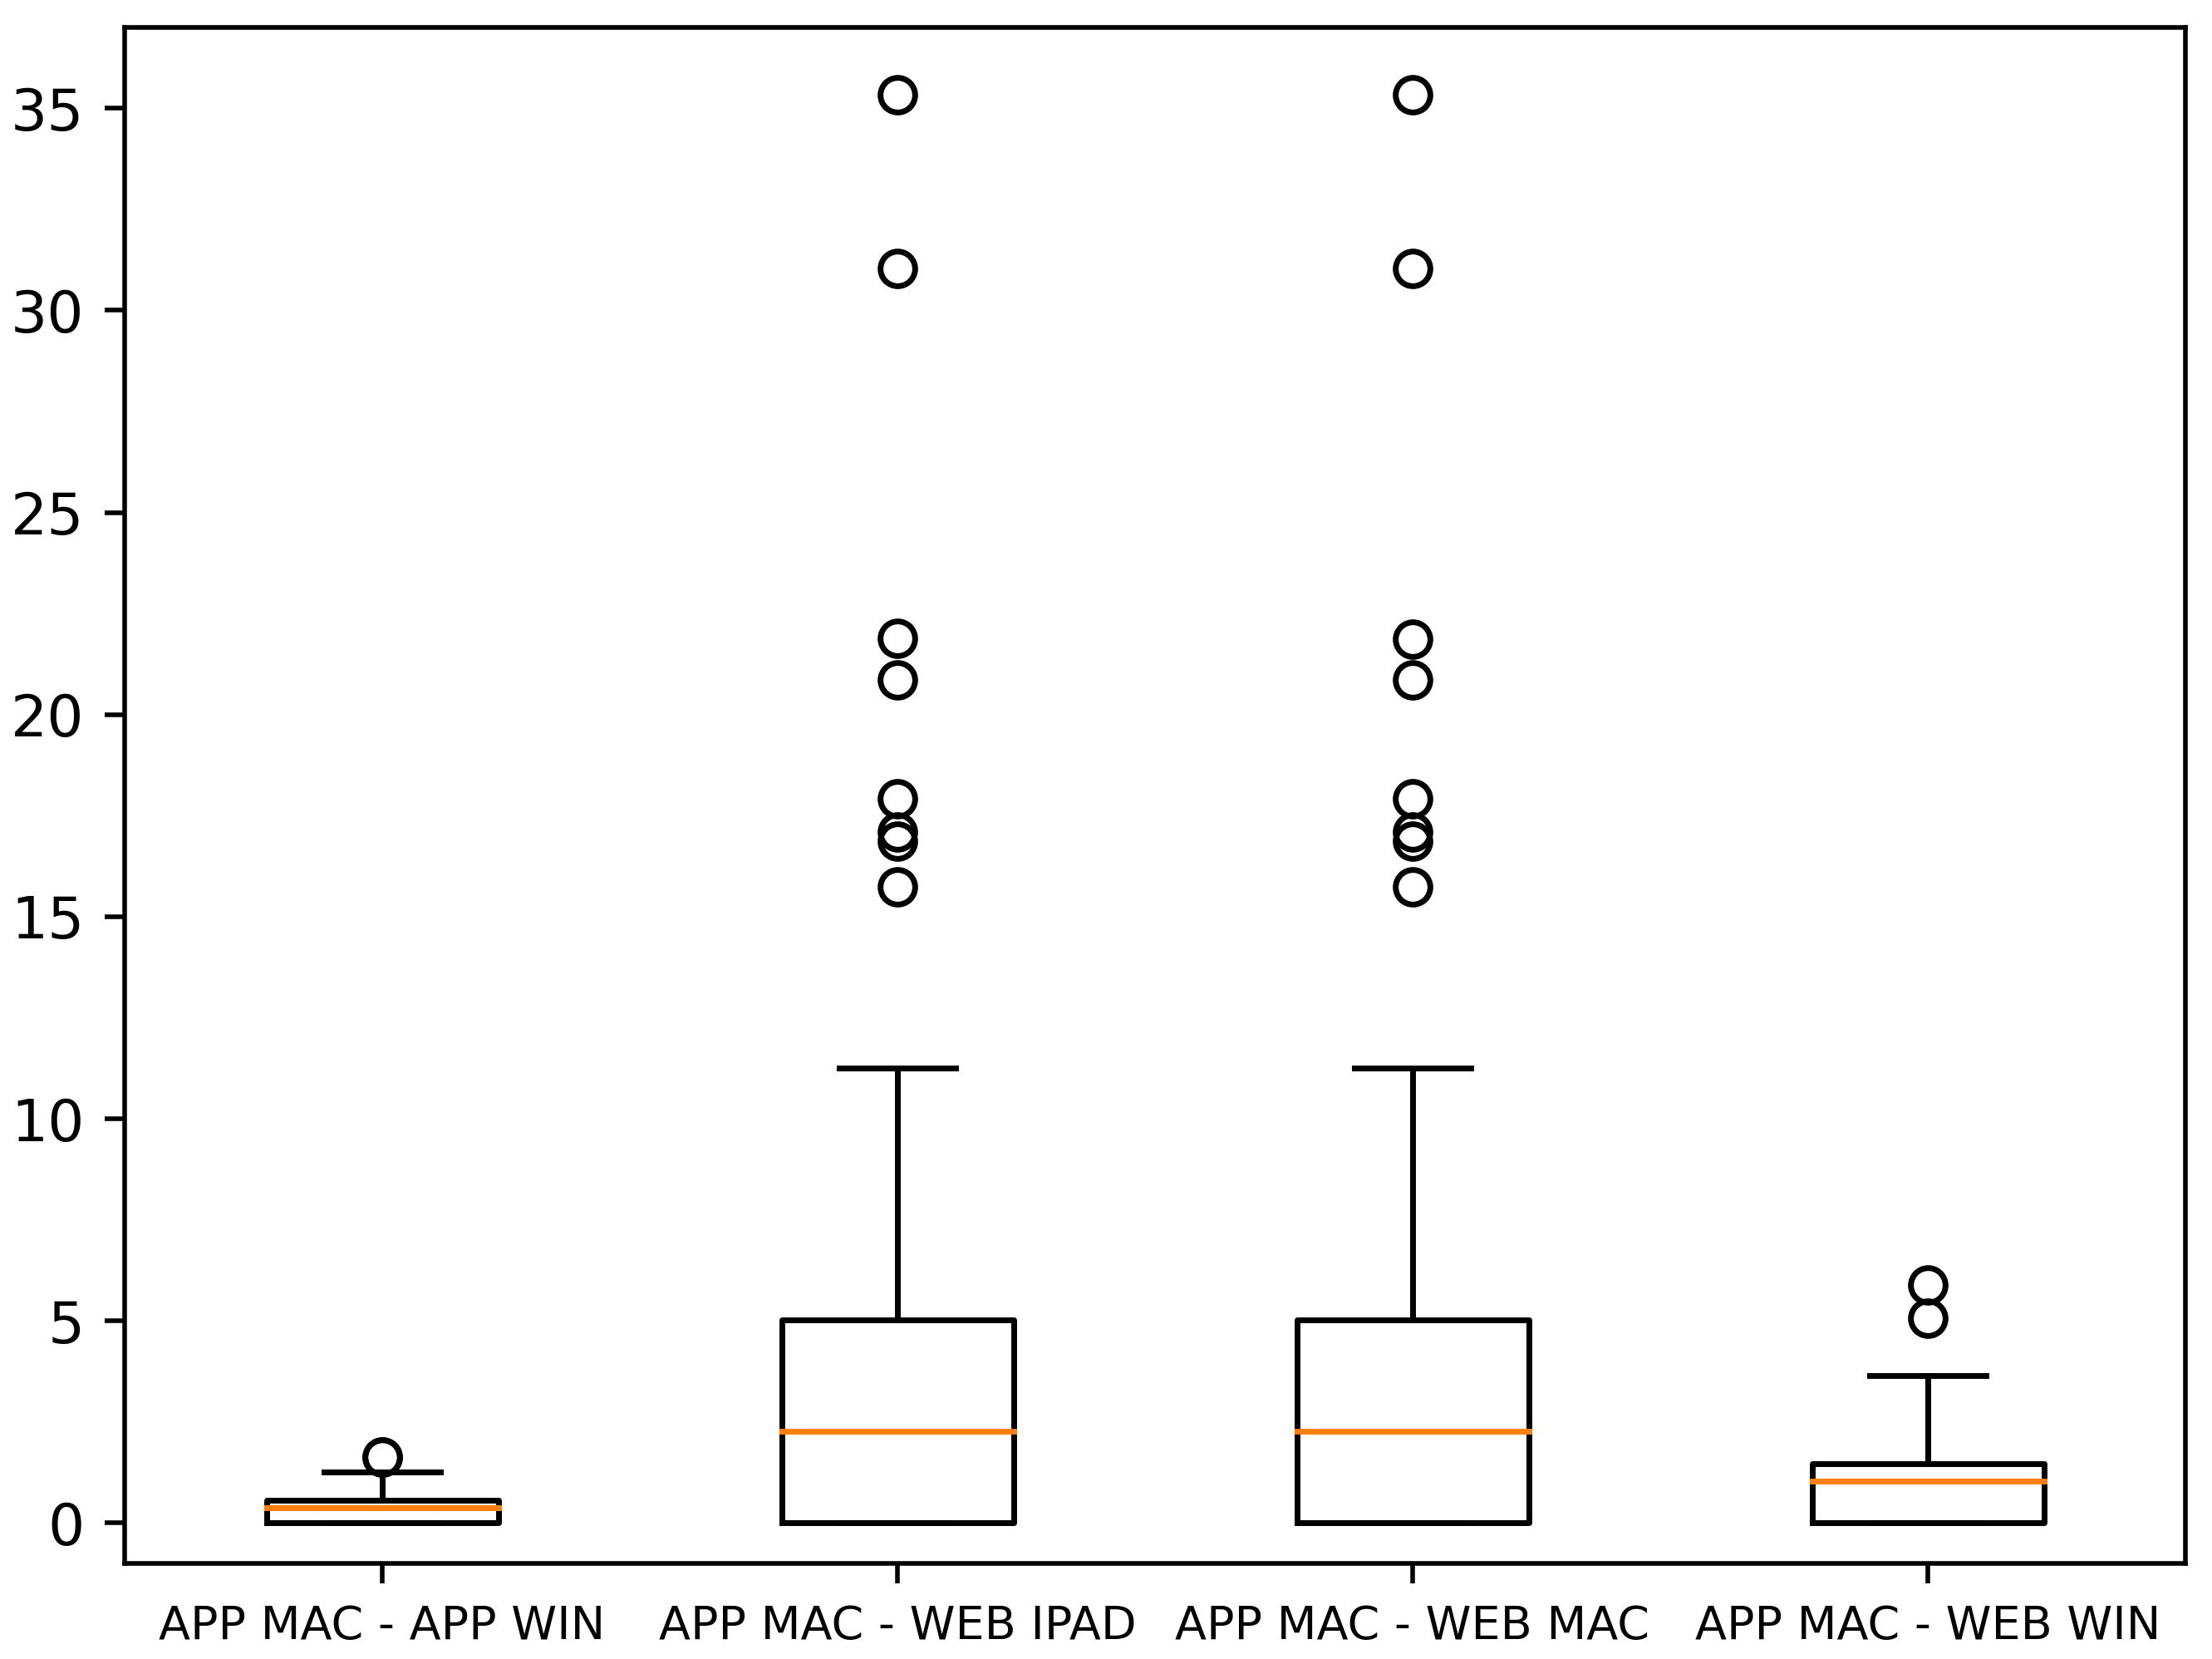
\includegraphics[width=8cm, height=8cm, keepaspectratio]{Immagini/MSE/Immagine1.png}\hspace{1em}
    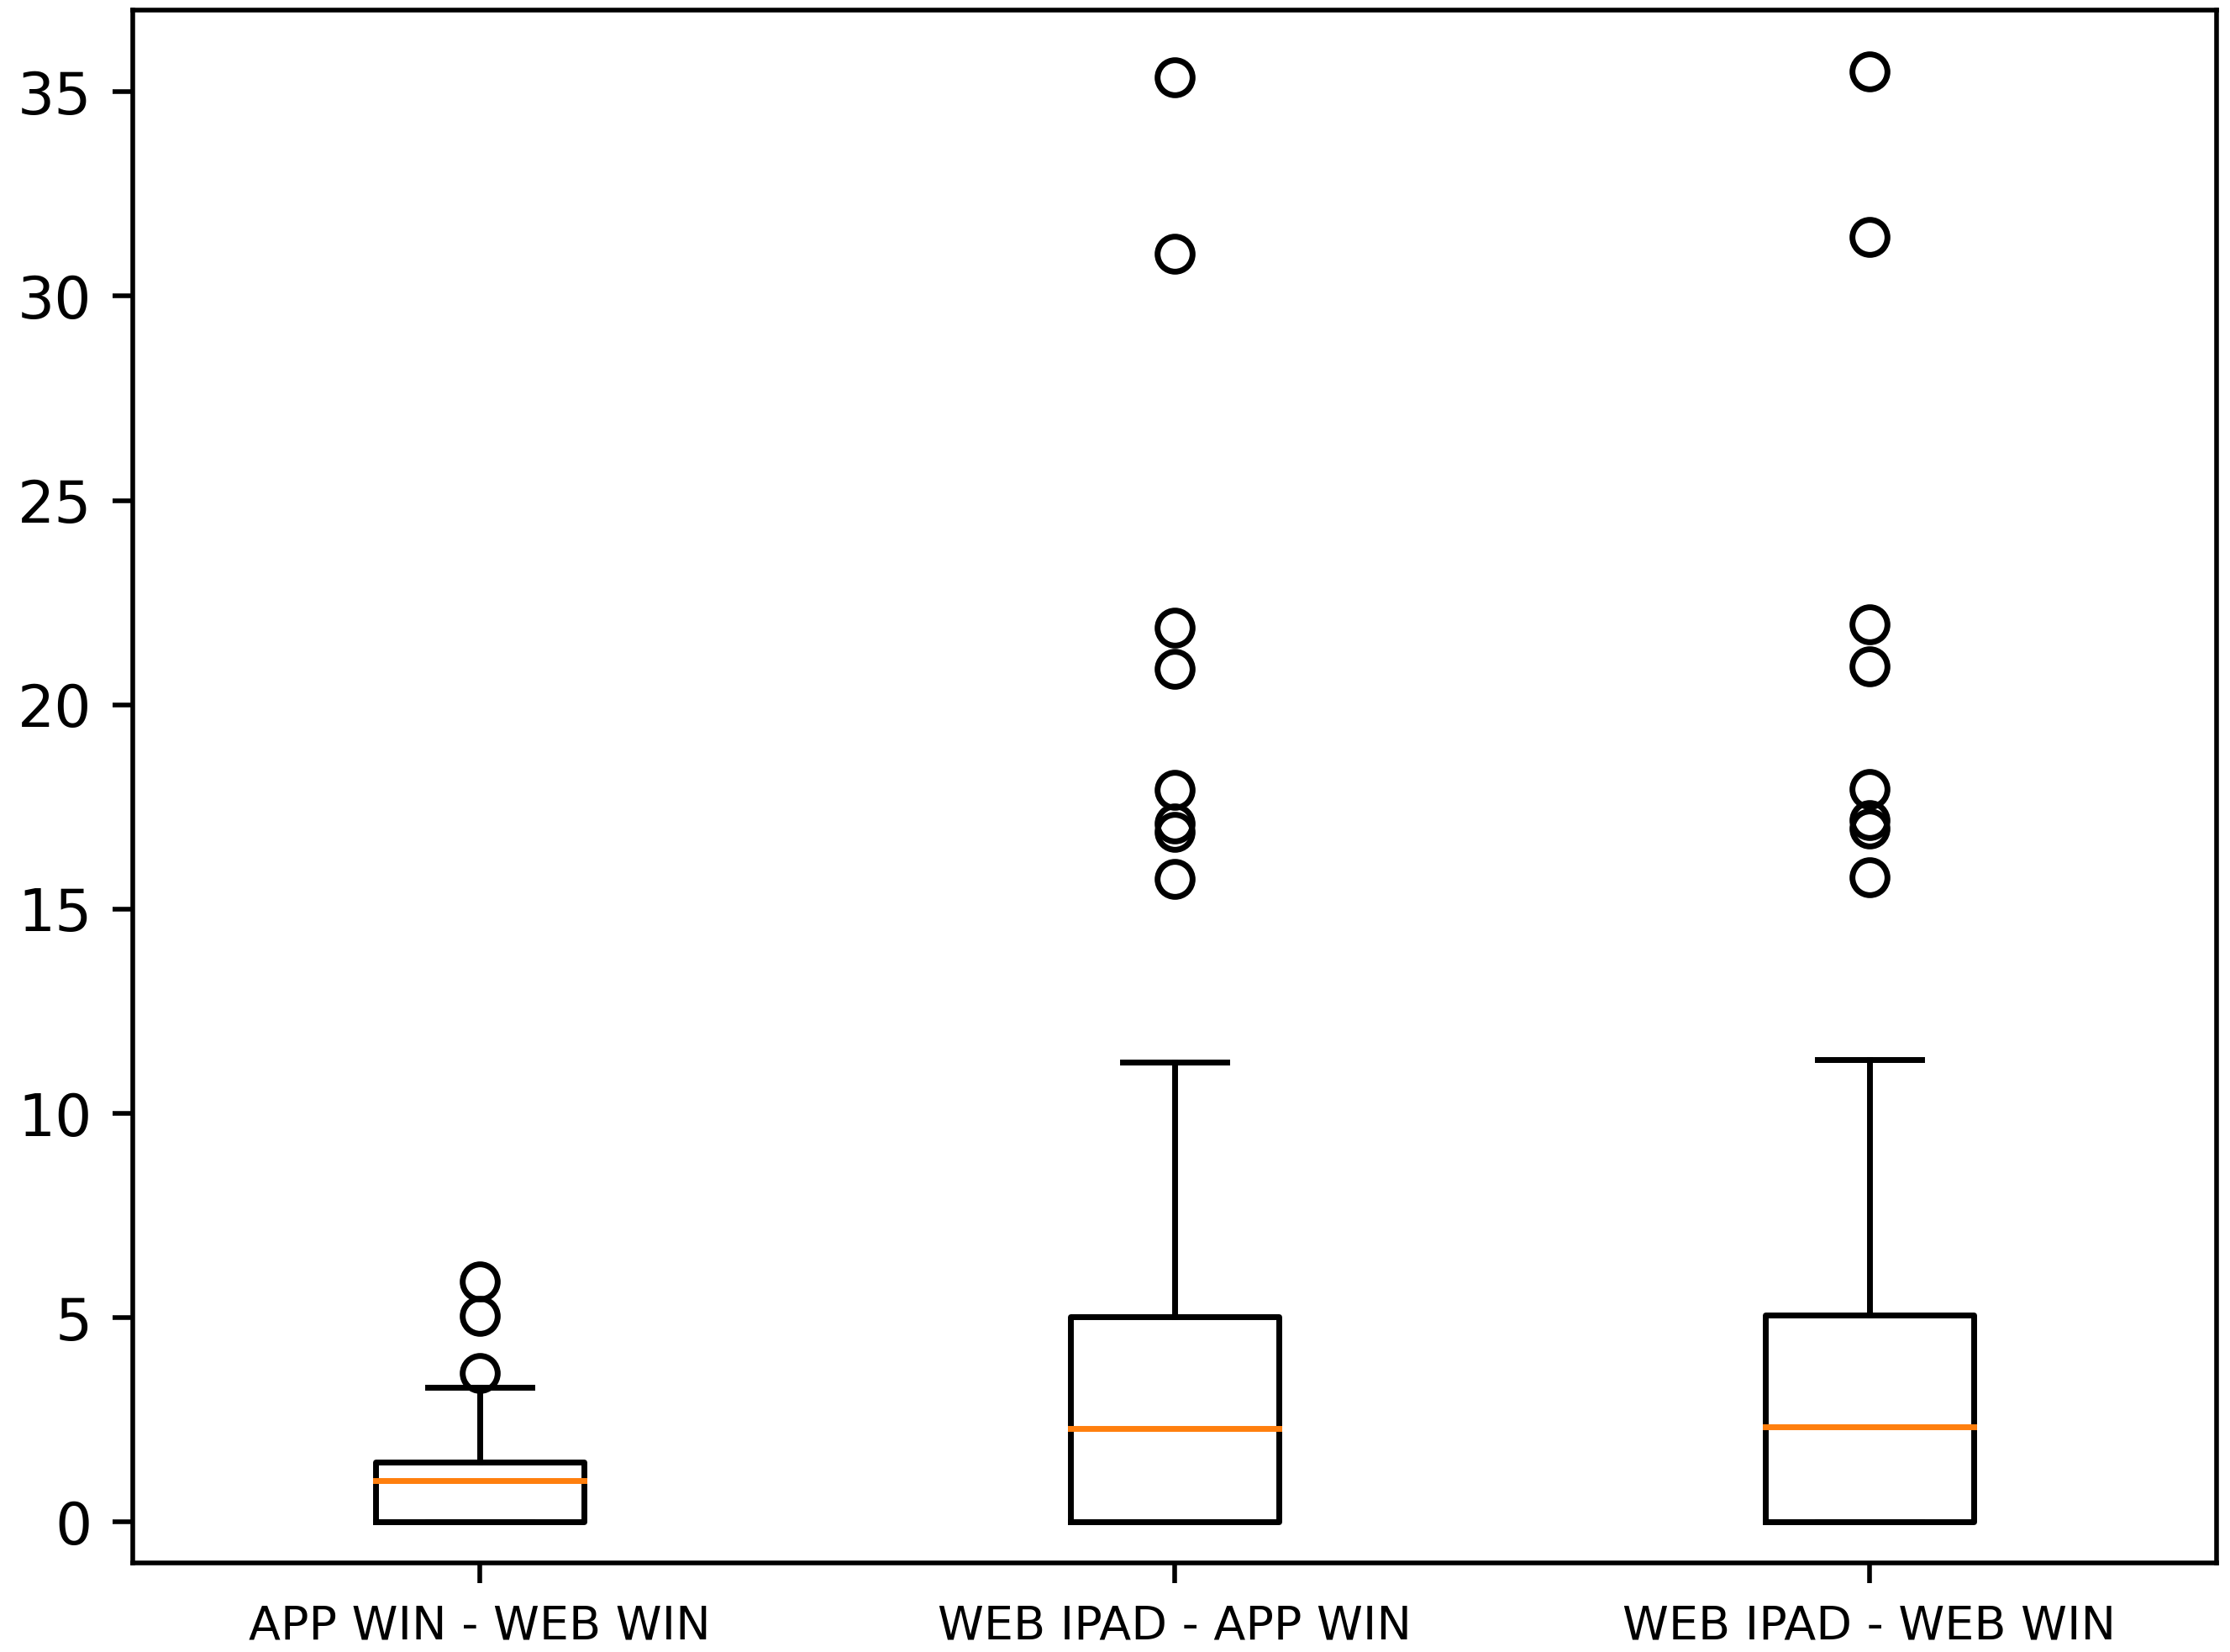
\includegraphics[width=8cm, height=8cm, keepaspectratio]{Immagini/MSE/Immagine2.png}\\\vspace{1em}
    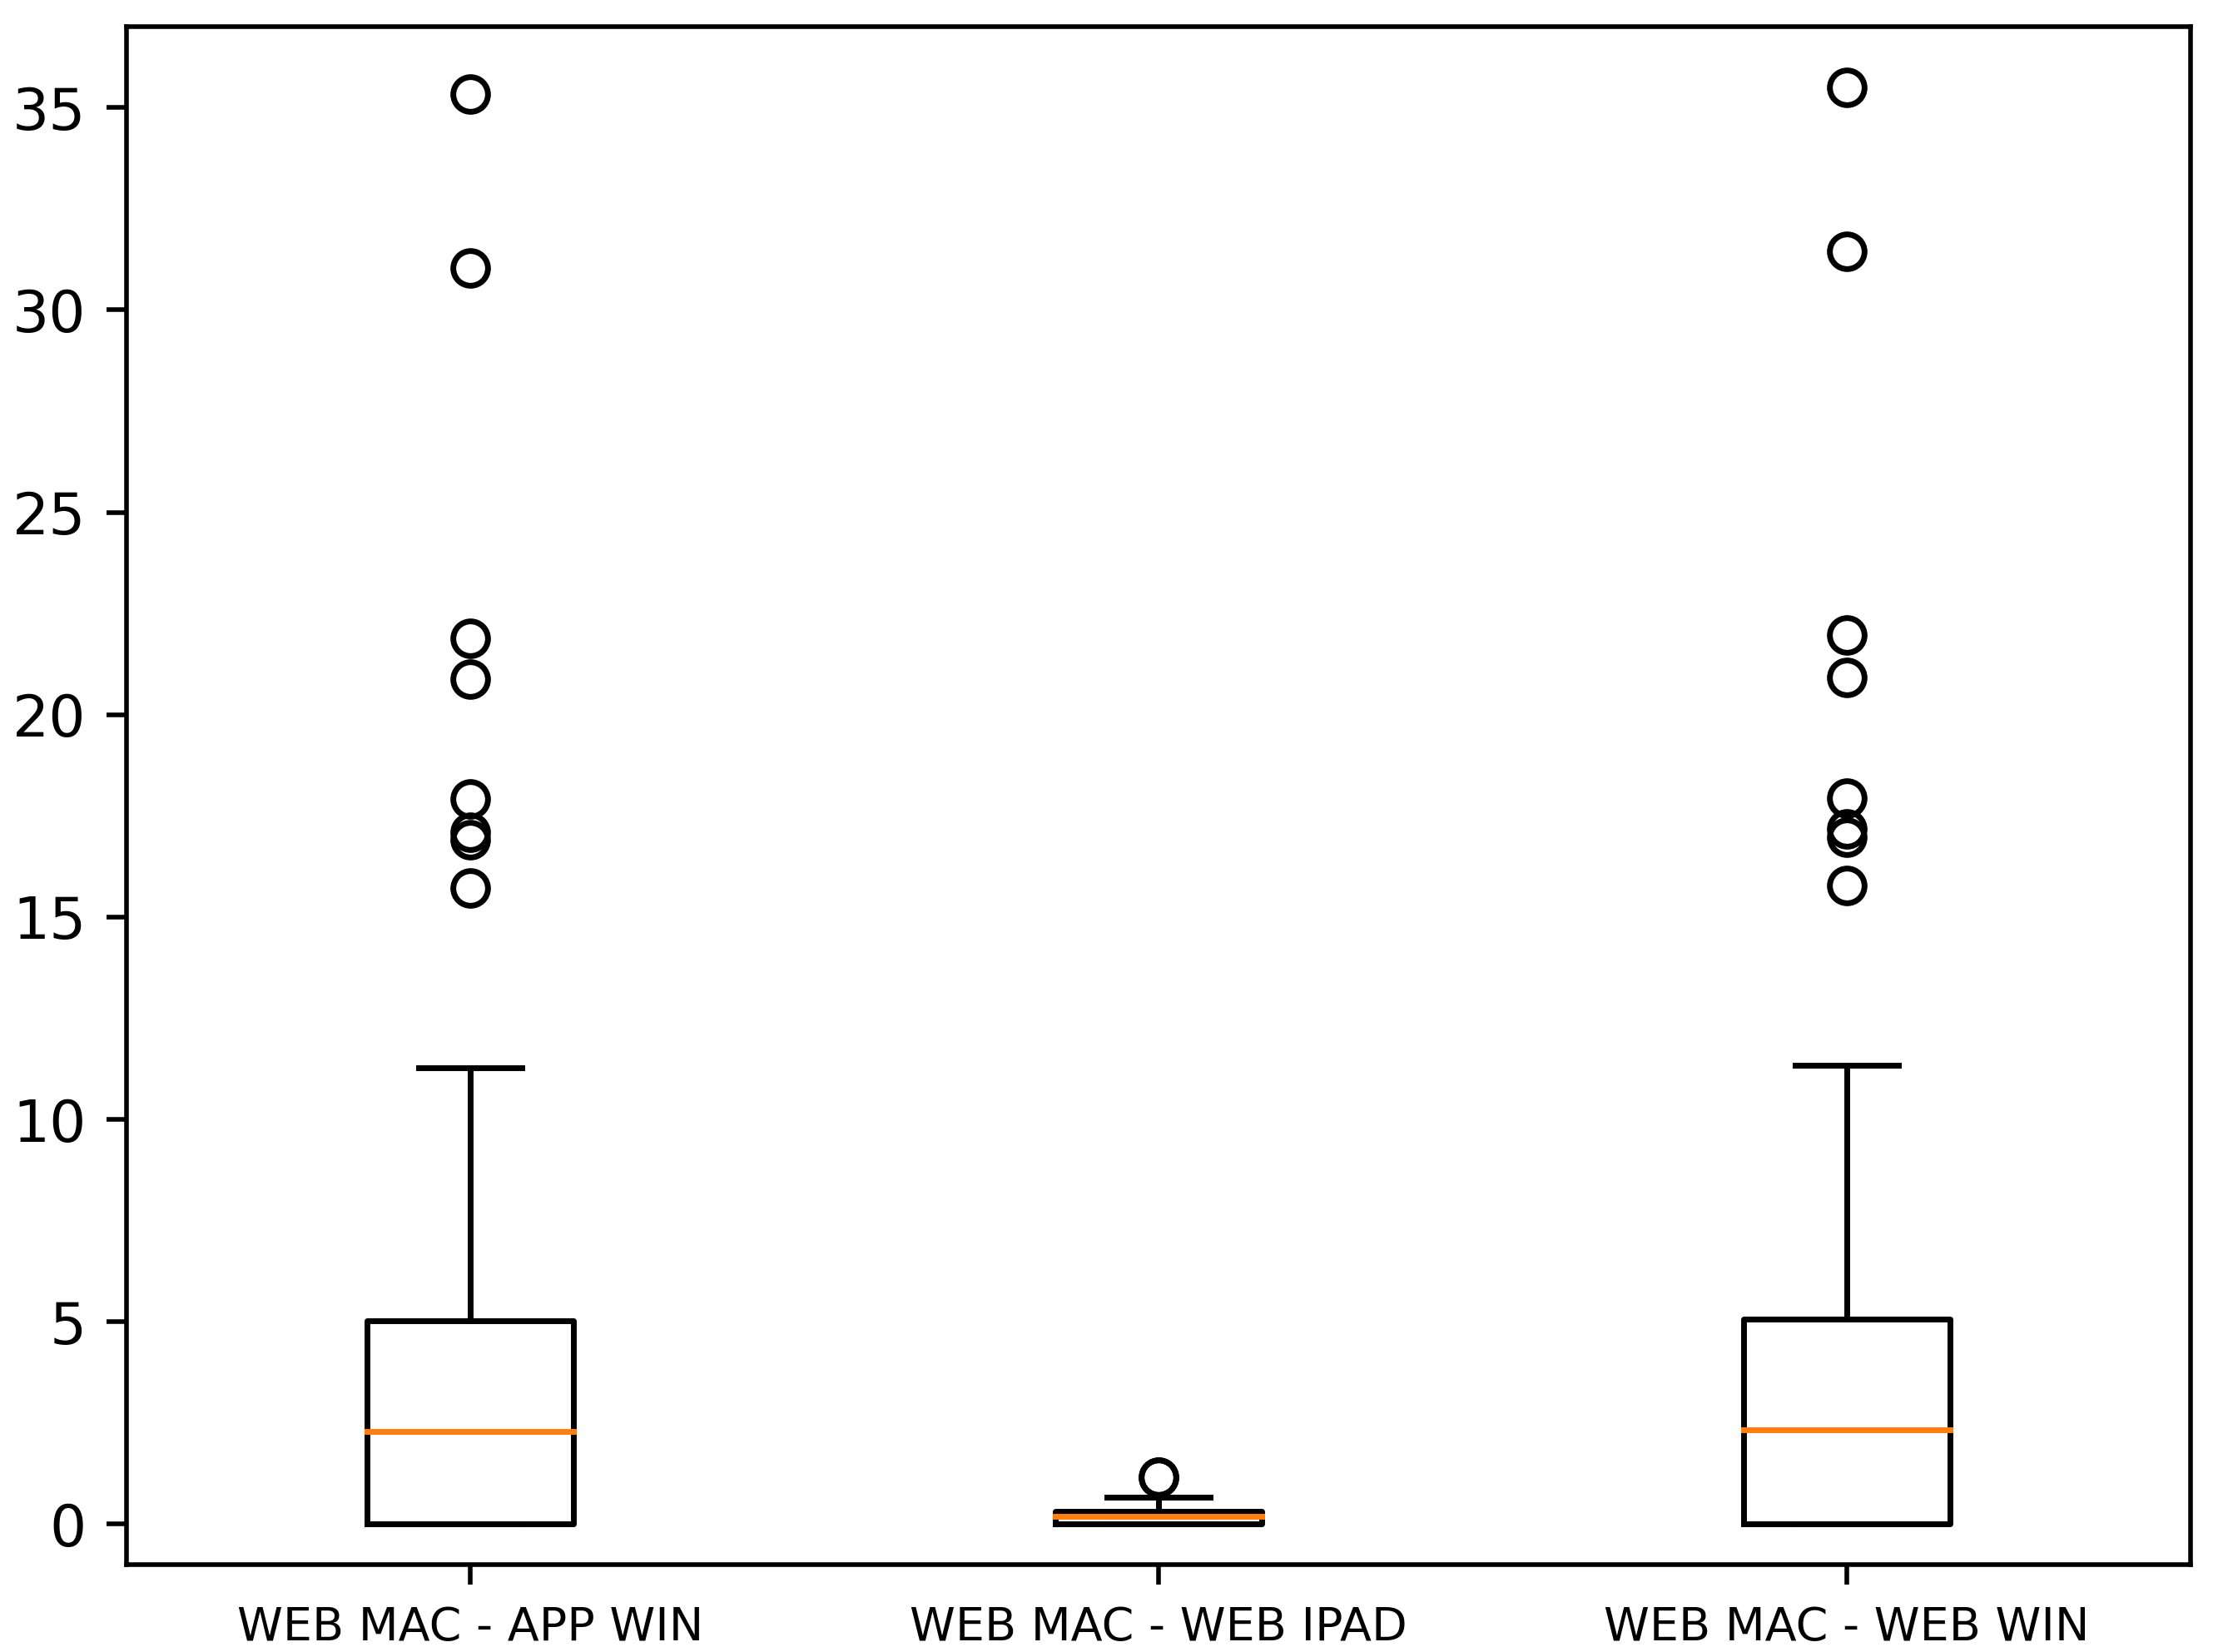
\includegraphics[width=8cm, height=8cm, keepaspectratio]{Immagini/MSE/Immagine3.png}
    \captionof{figure}{Valori del \textit{Mean Square Error} per coppie di metodi di condivisione. I \textit{boxplot} ottenuti sono così formati: la linea arancione corrisponde alla mediana dei valori; il rettangolo costituisce l'intervallo interquartile; la linea sopra indica il terzo quartile mentre i cerchi corrispondono agli \textit{outliers}.}
    \label{fig:mse_results}
\endgroup

% \begin{figure}[h!]
%     \centering
%     \subfloat[][]{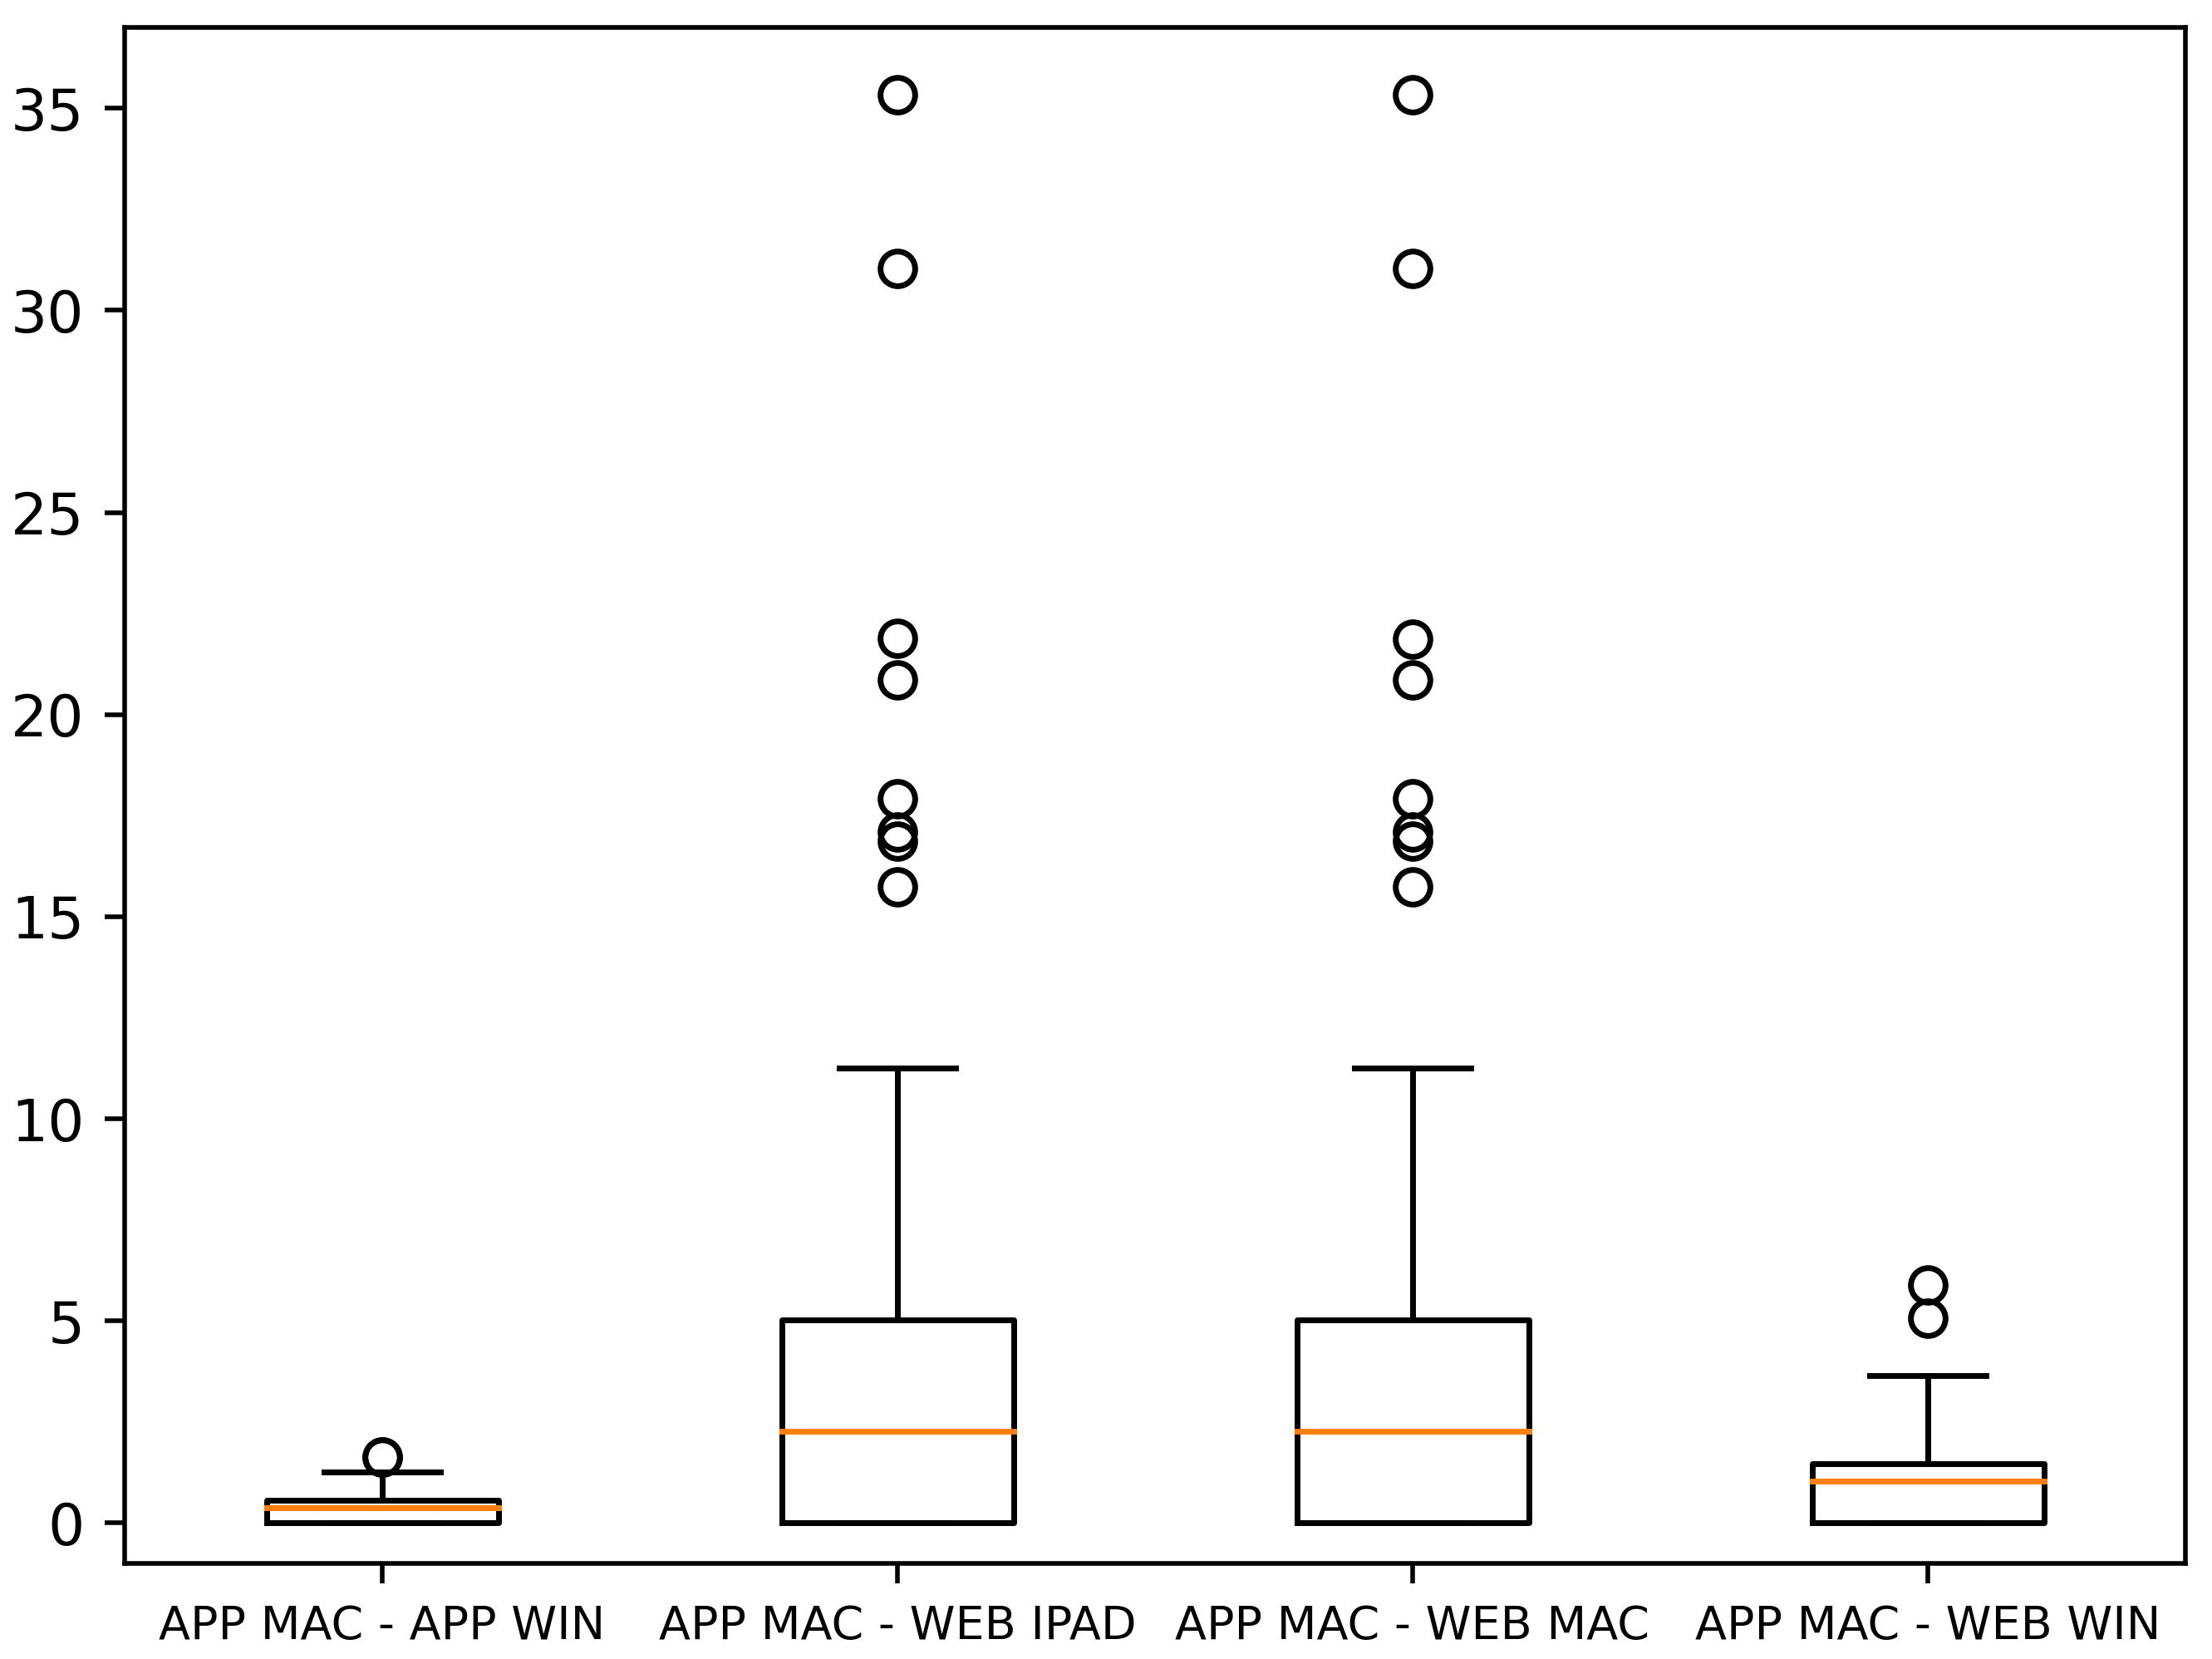
\includegraphics[width=8cm, height=8cm, keepaspectratio]{Immagini/MSE/Immagine1.png}}\hspace{1em}
%     \subfloat[][]{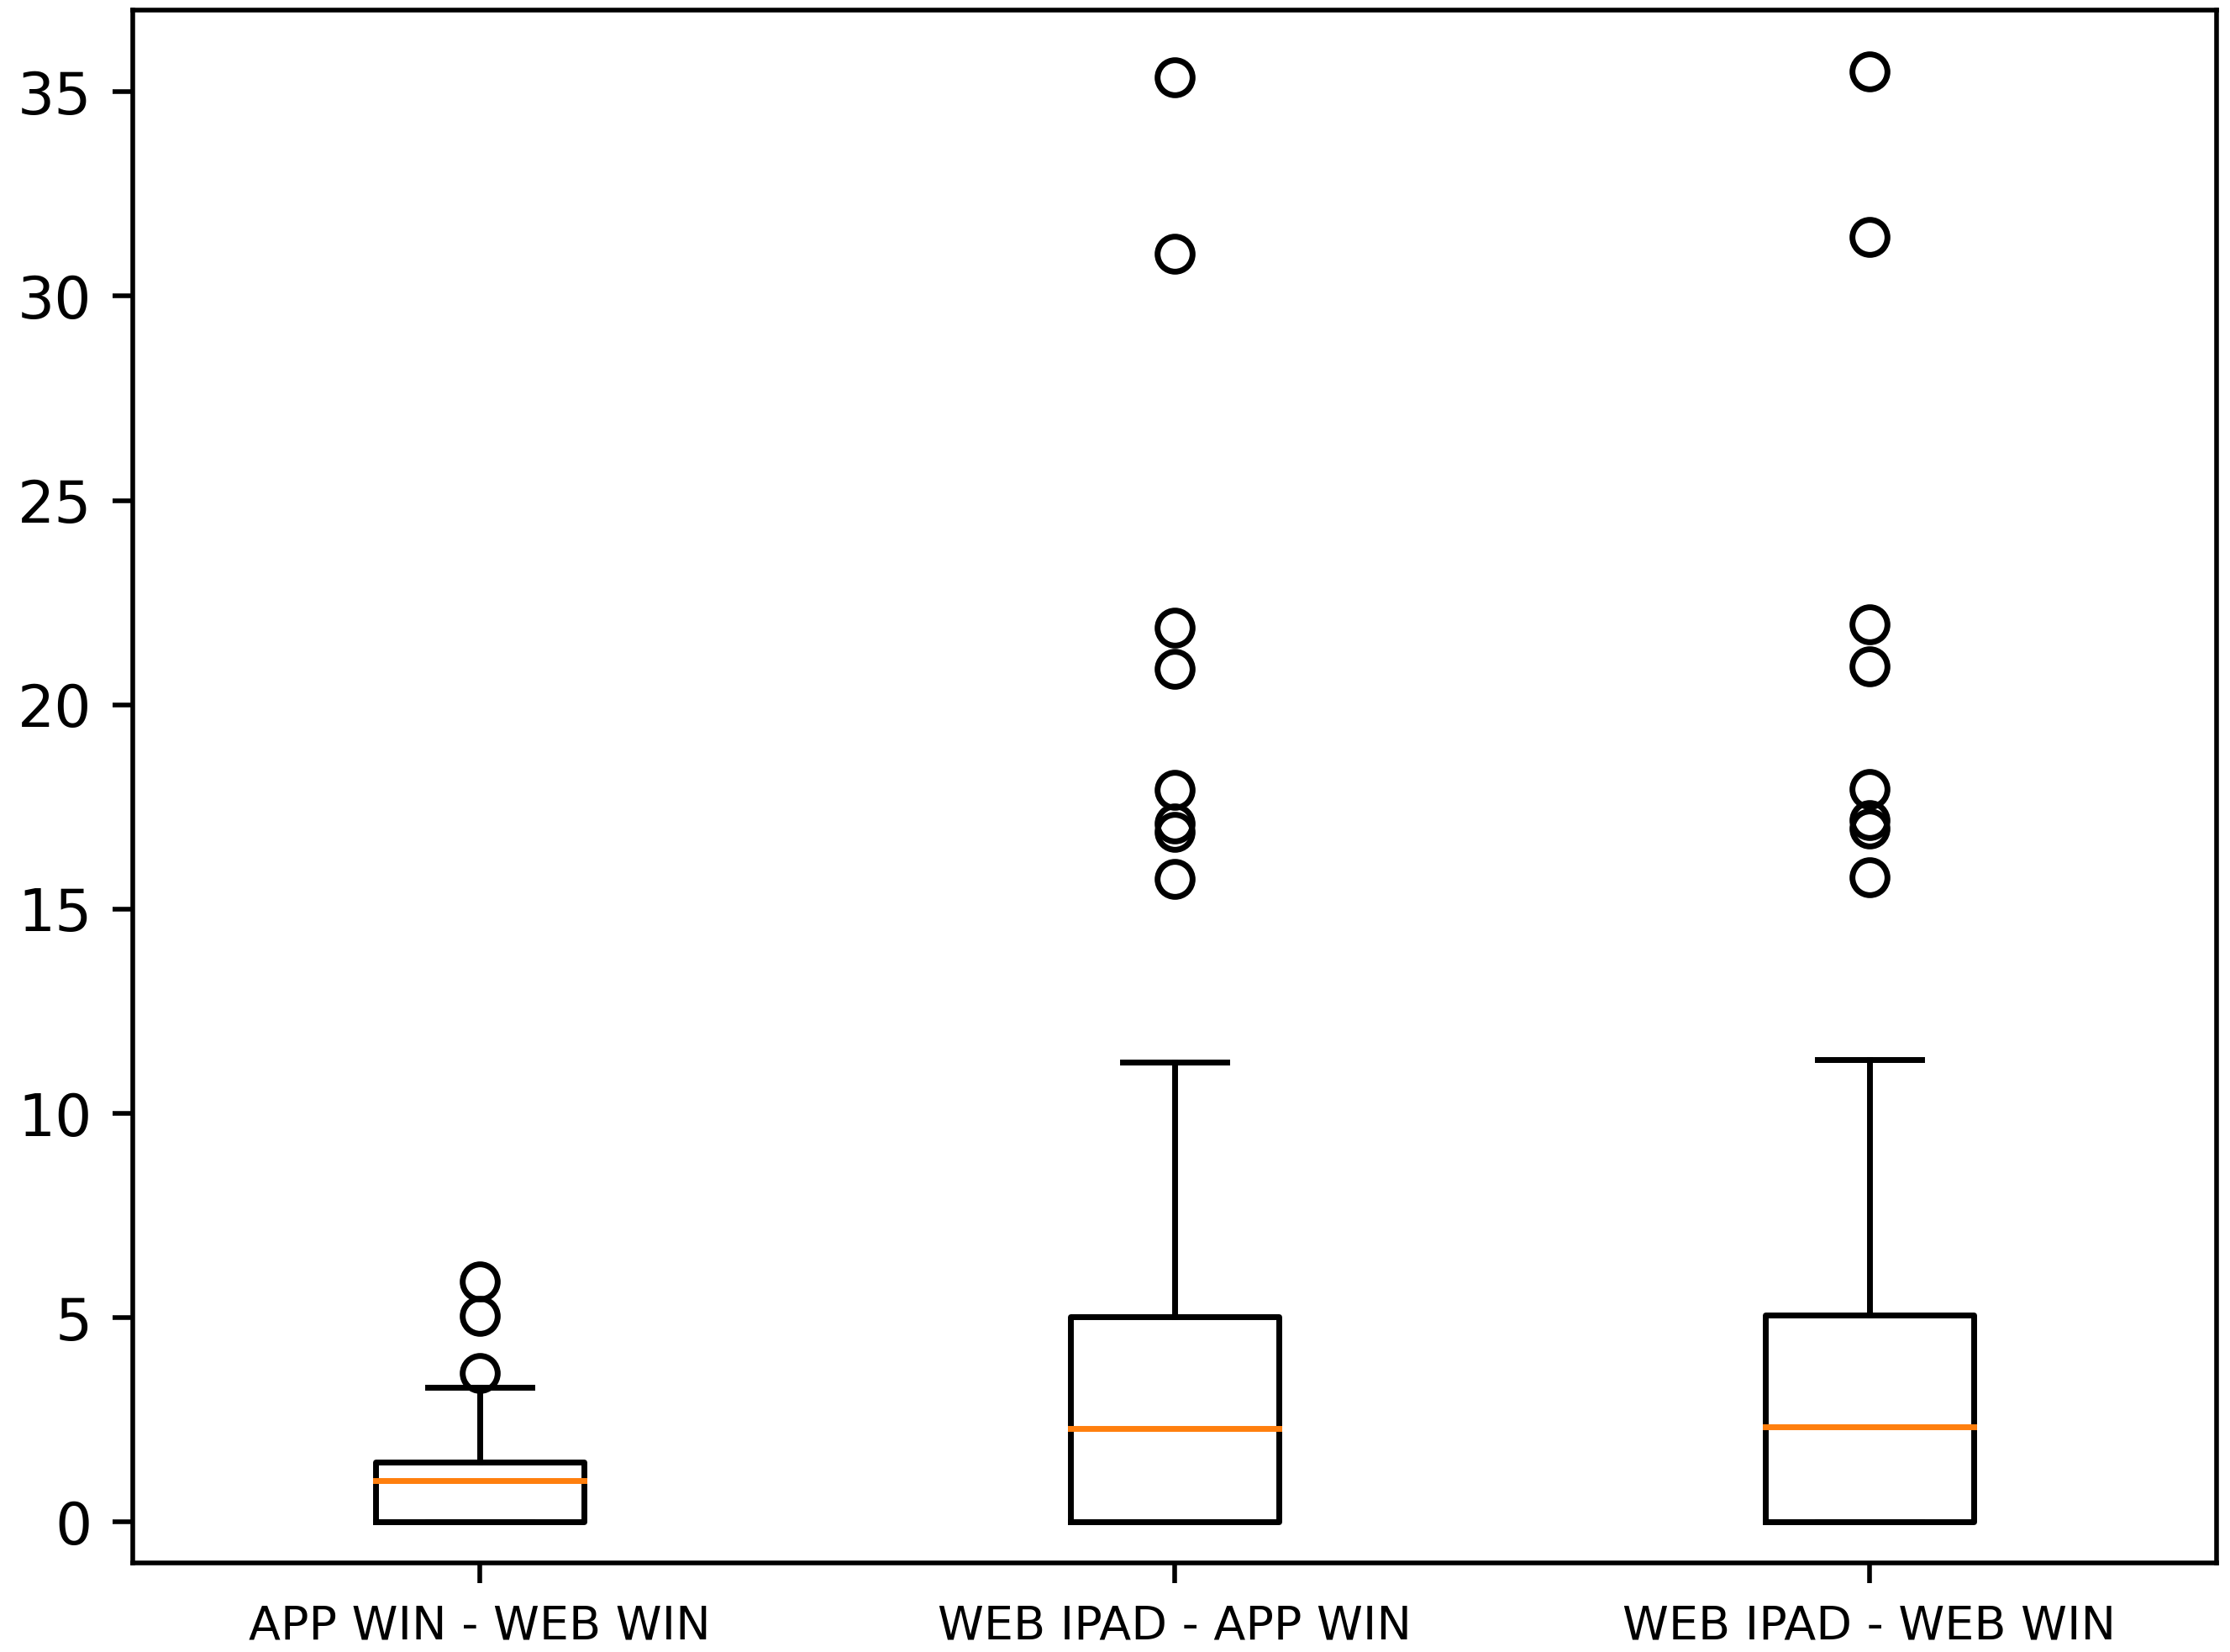
\includegraphics[width=8cm, height=8cm, keepaspectratio]{Immagini/MSE/Immagine2.png}}\\\vspace{1em}
%     \subfloat[][]{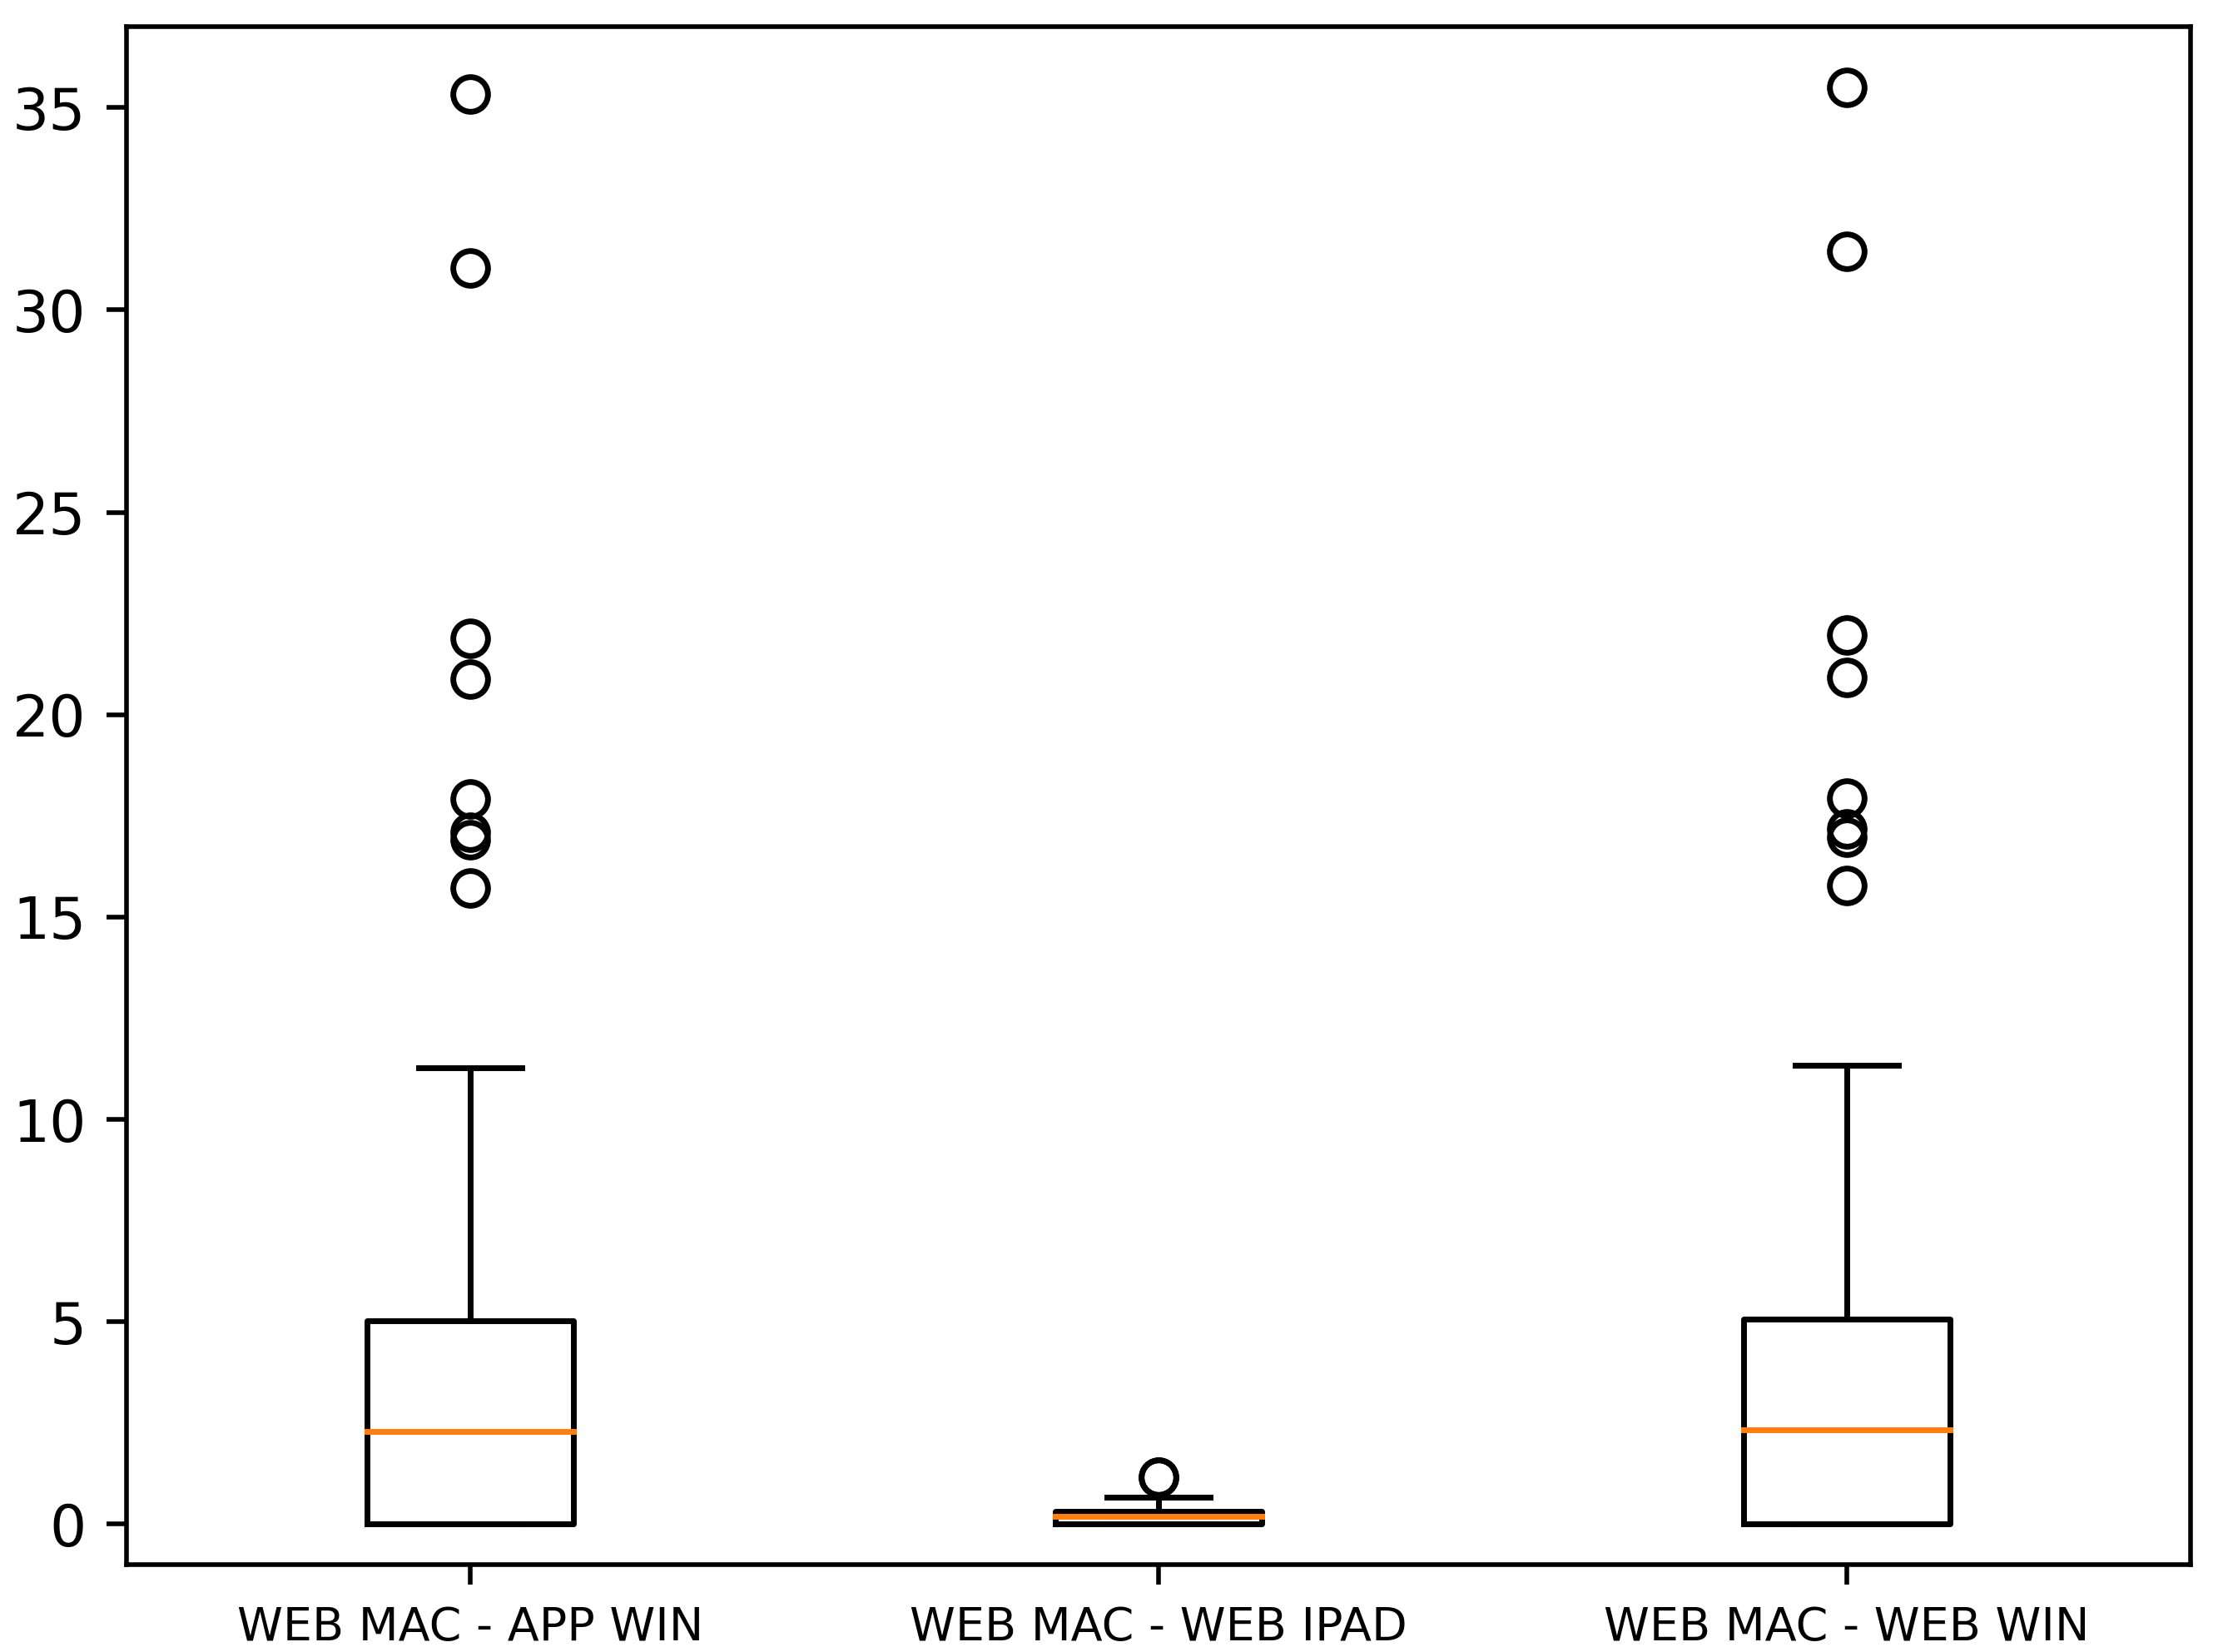
\includegraphics[width=8cm, height=8cm, keepaspectratio]{Immagini/MSE/Immagine3.png}}
%     \caption{Valori del \textit{Mean Square Error} per coppie di metodi di condivisione. I \textit{boxplot} ottenuti sono così formati: la linea arancione corrisponde alla mediana dei valori; il rettangolo costituisce l'intervallo interquartile; le linee sopra indicano il primo quartile mentre i cerchi corrispondono agli \textit{outliers}.}
%     \label{fig:mse_results}
% \end{figure}

\vspace{2em}

Guardando ai grafici ottenuti per il \textit{Peak Signal-to-Noise Ratio} in Fig.~\ref{fig:psnr_results} e in particolare all'elevato range di valori, si evidenzia come il livello di compressione applicato sulle immagini da WhatsApp non abbia particolarmente impattato sulla loro qualità. Notare come le coppie di immagini per cui il calcolo del MSE ha dato risultato 0 non siano presenti per le ragioni citate nel capitolo precedente. I pattern riscontrati per i risultati del MSE sono identificabili anche nel caso del PSNR.\\

% \begin{figure}[h!]
%     \centering
%     \subfloat[][]{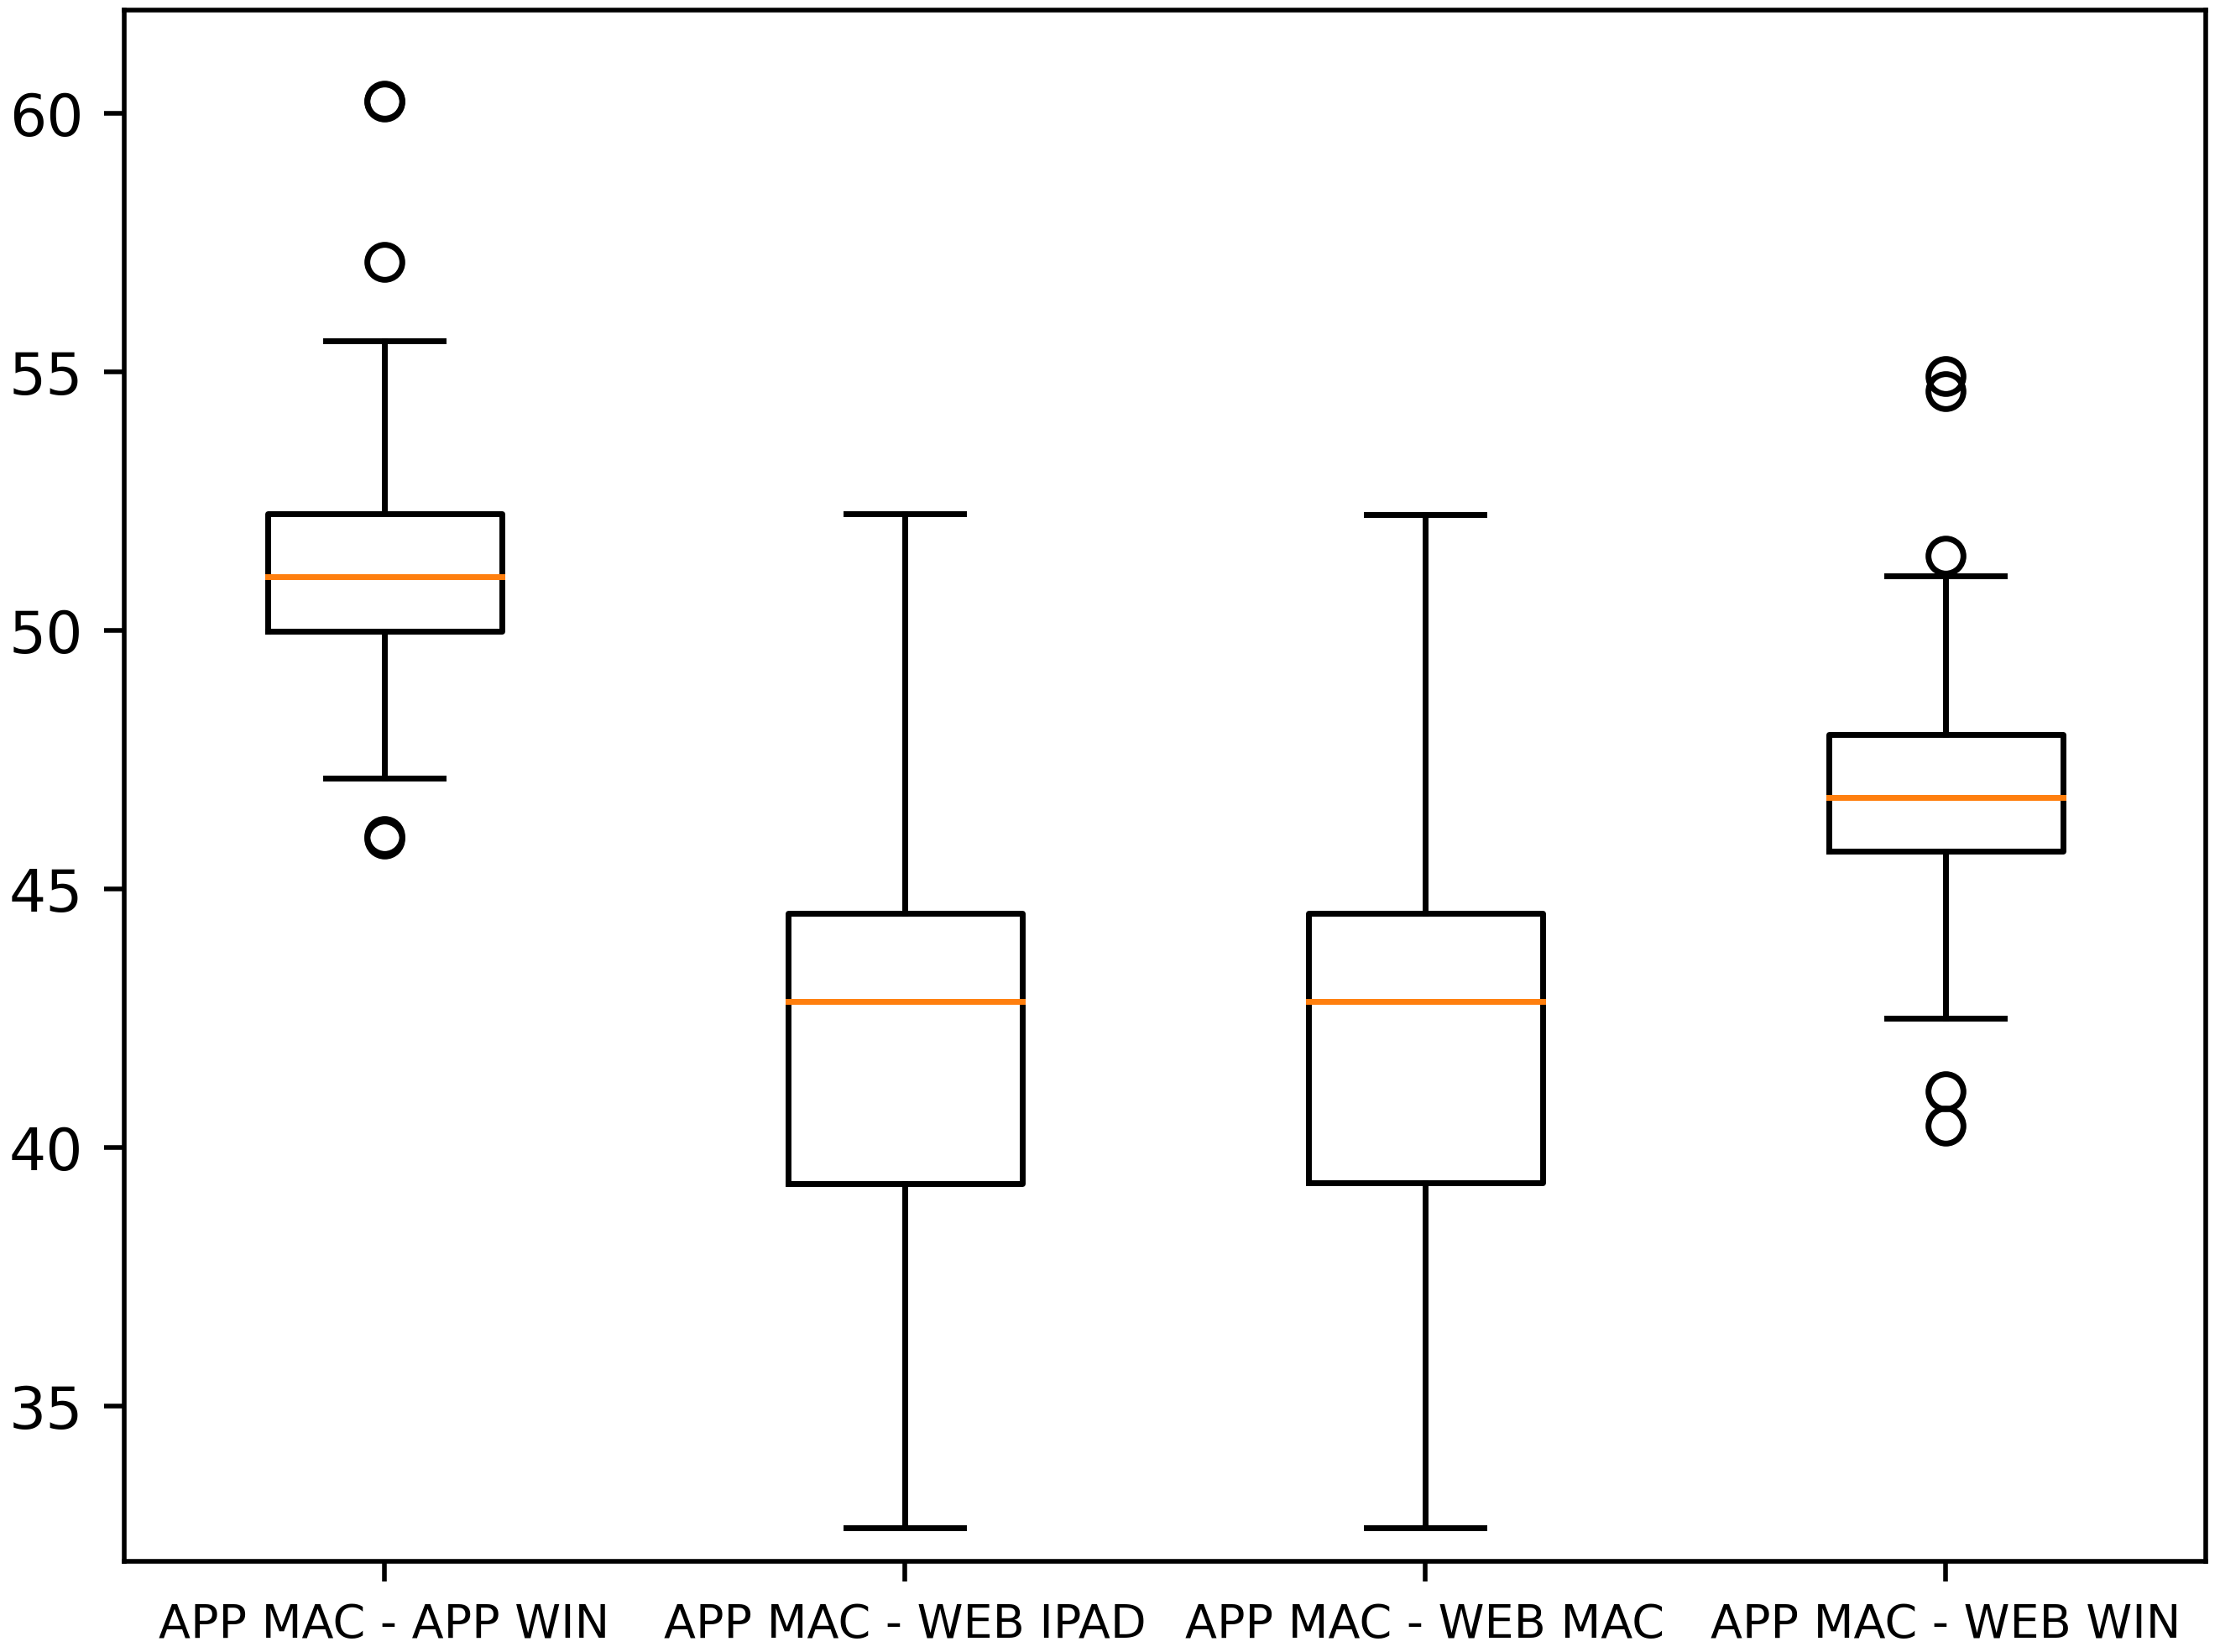
\includegraphics[width=8cm, height=8cm, keepaspectratio]{Immagini/PSNR/Immagine1.png}}\hspace{1em}
%     \subfloat[][]{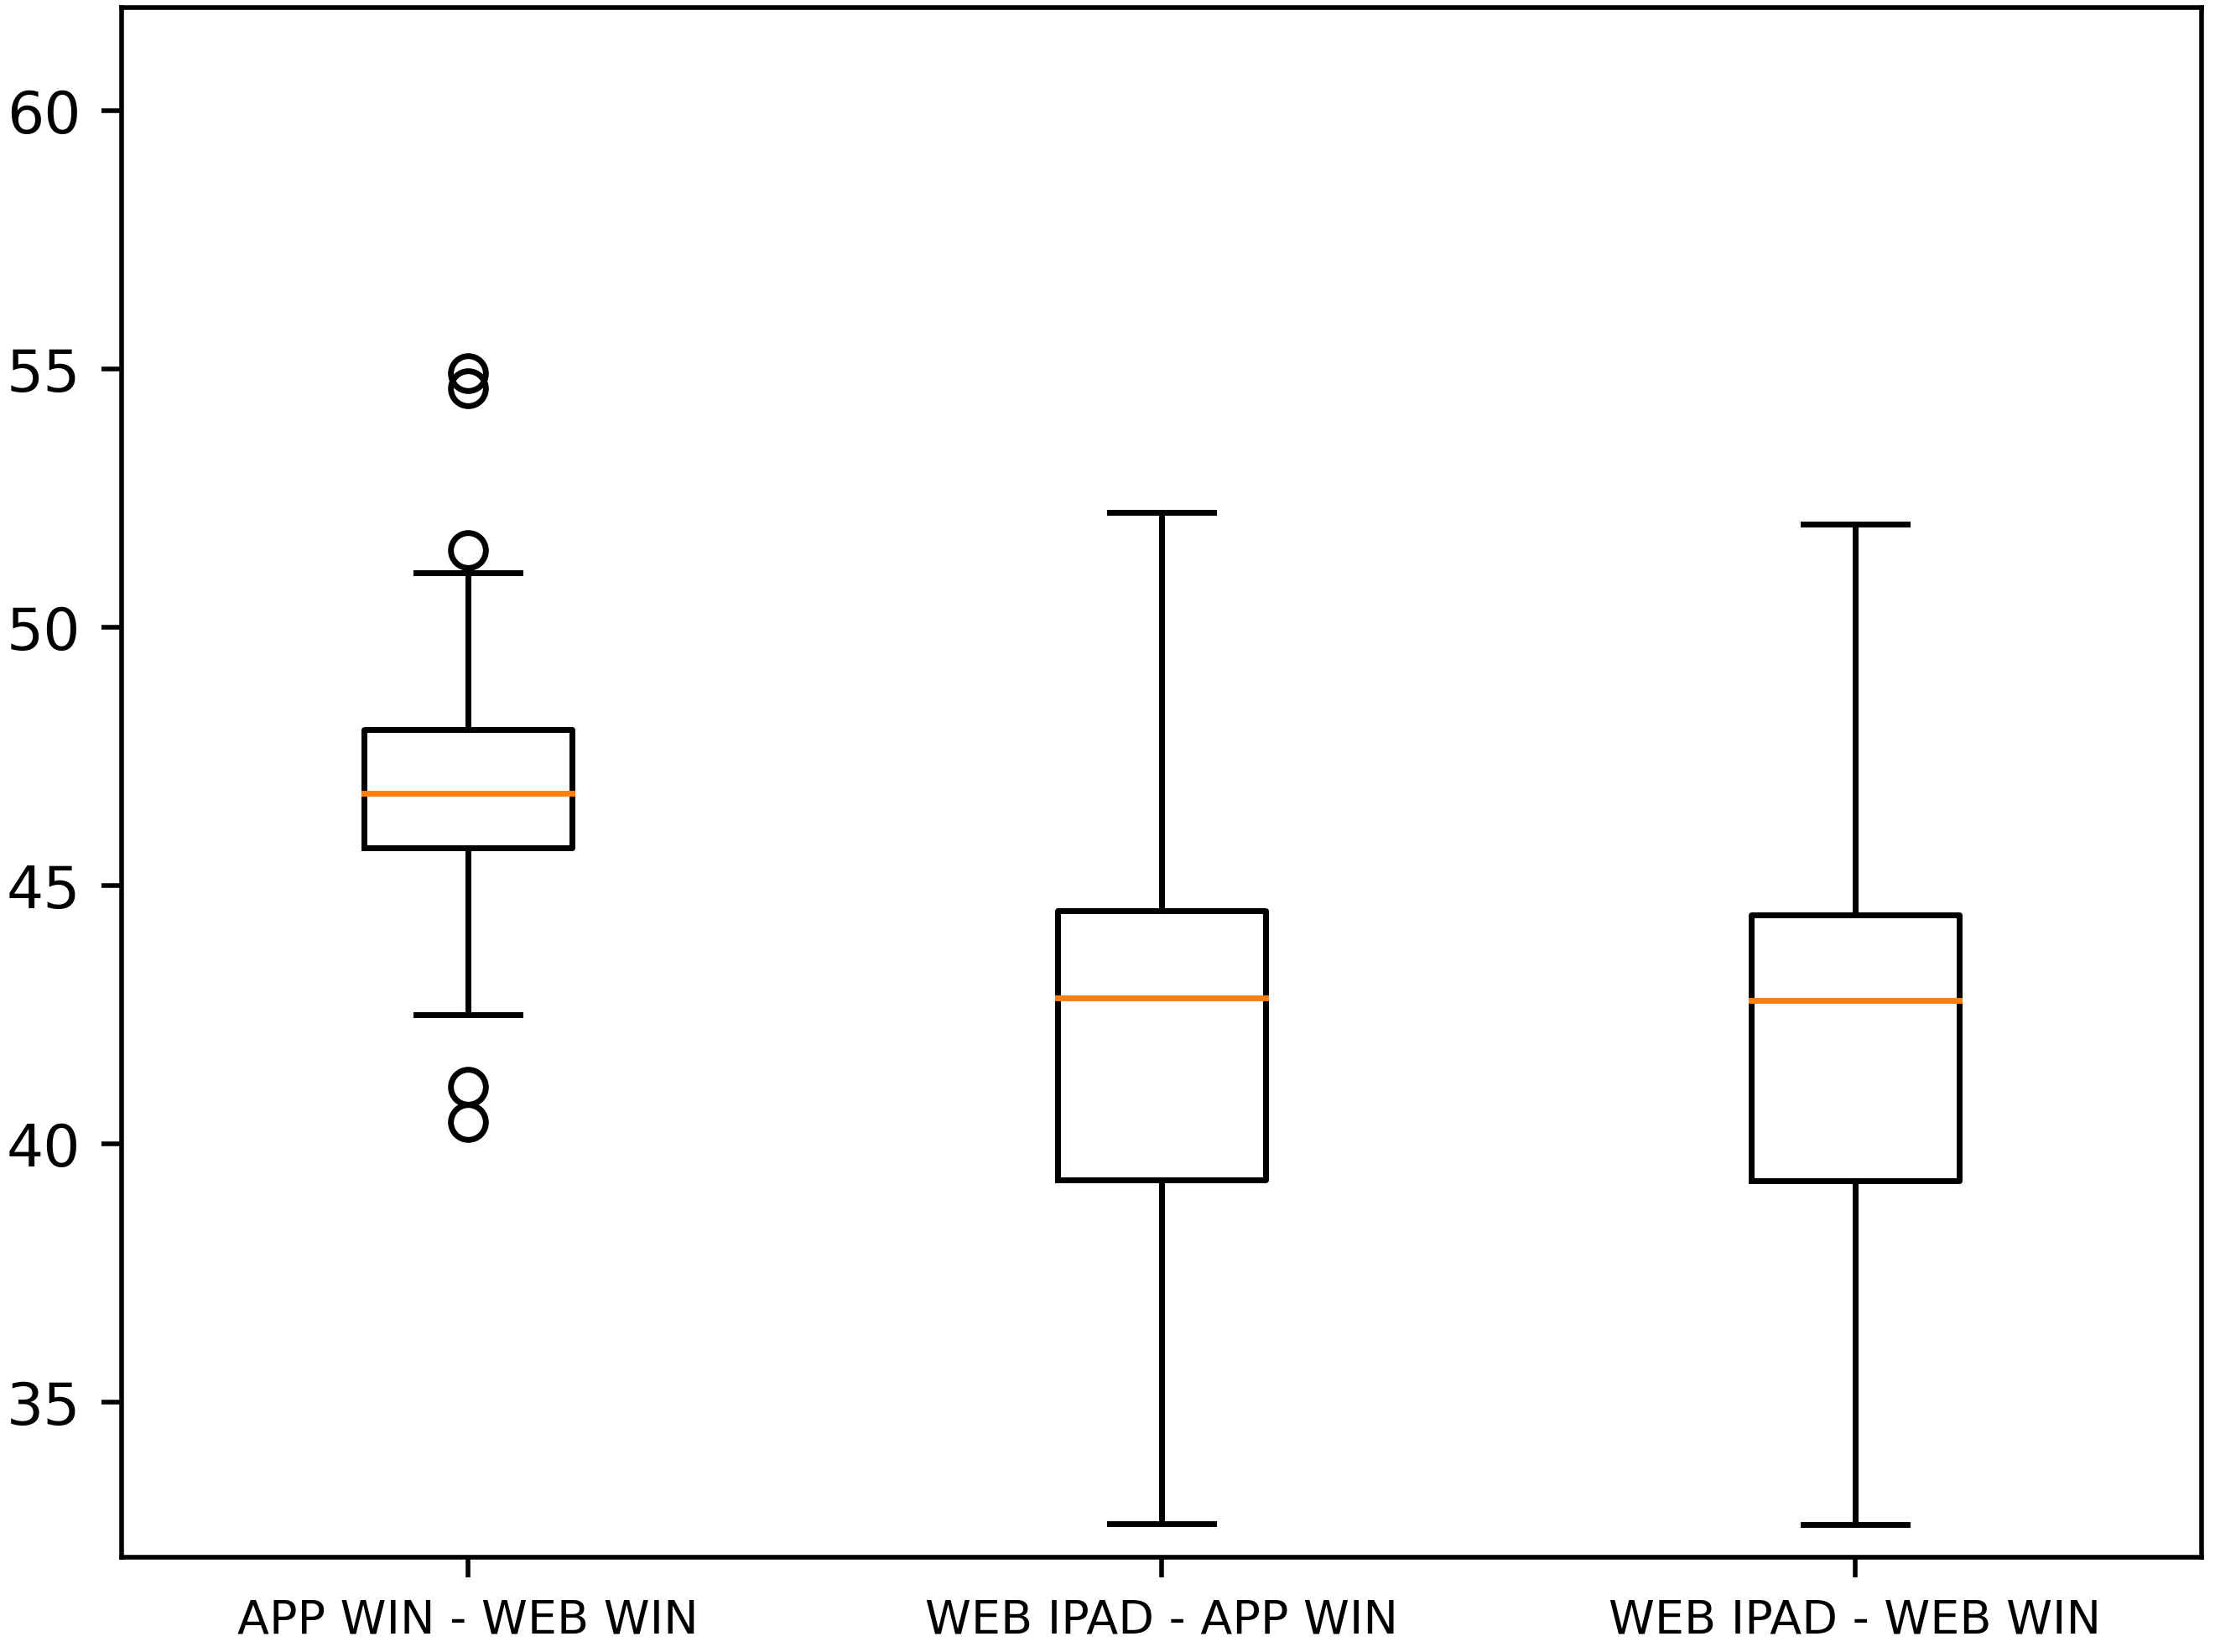
\includegraphics[width=8cm, height=8cm, keepaspectratio]{Immagini/PSNR/Immagine2.png}}\\\vspace{1em}
%     \subfloat[][]{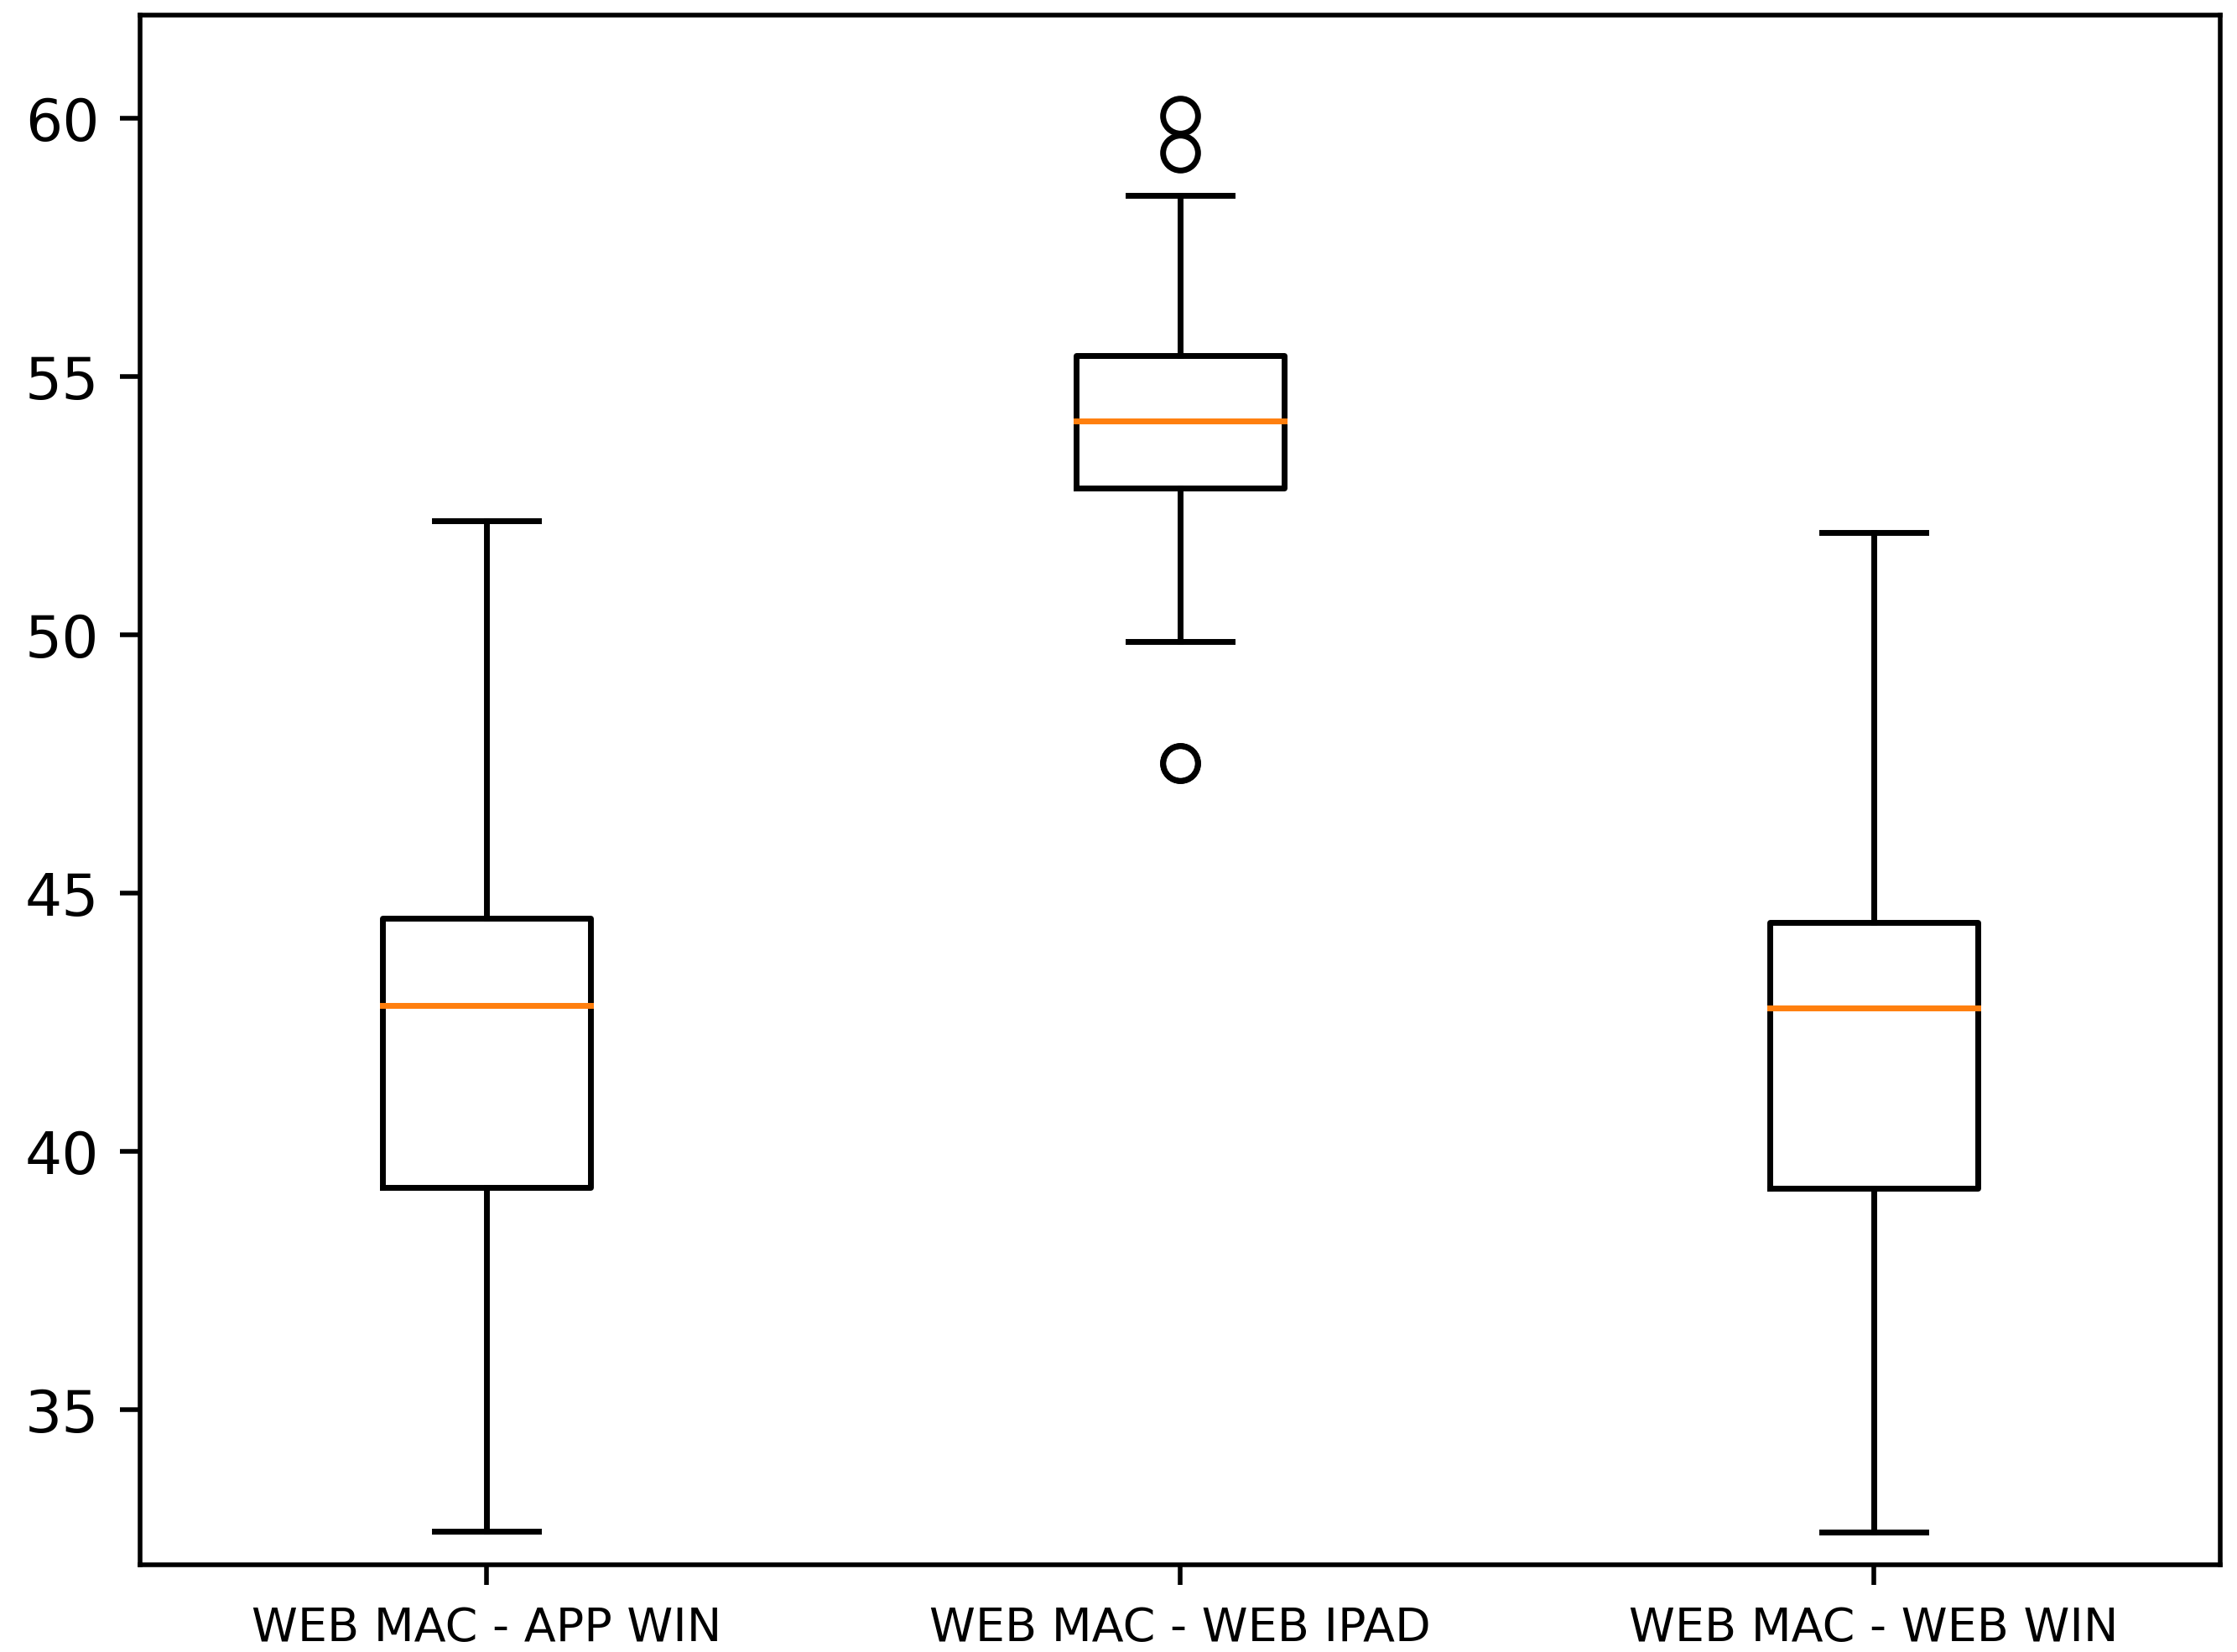
\includegraphics[width=8cm, height=8cm, keepaspectratio]{Immagini/PSNR/Immagine3.png}}\\
%     \caption{\textit{Boxplot} ricavati dal calcolo del PSNR}
%     \label{fig:psnr_results}
% \end{figure}

\begingroup
    \centering
    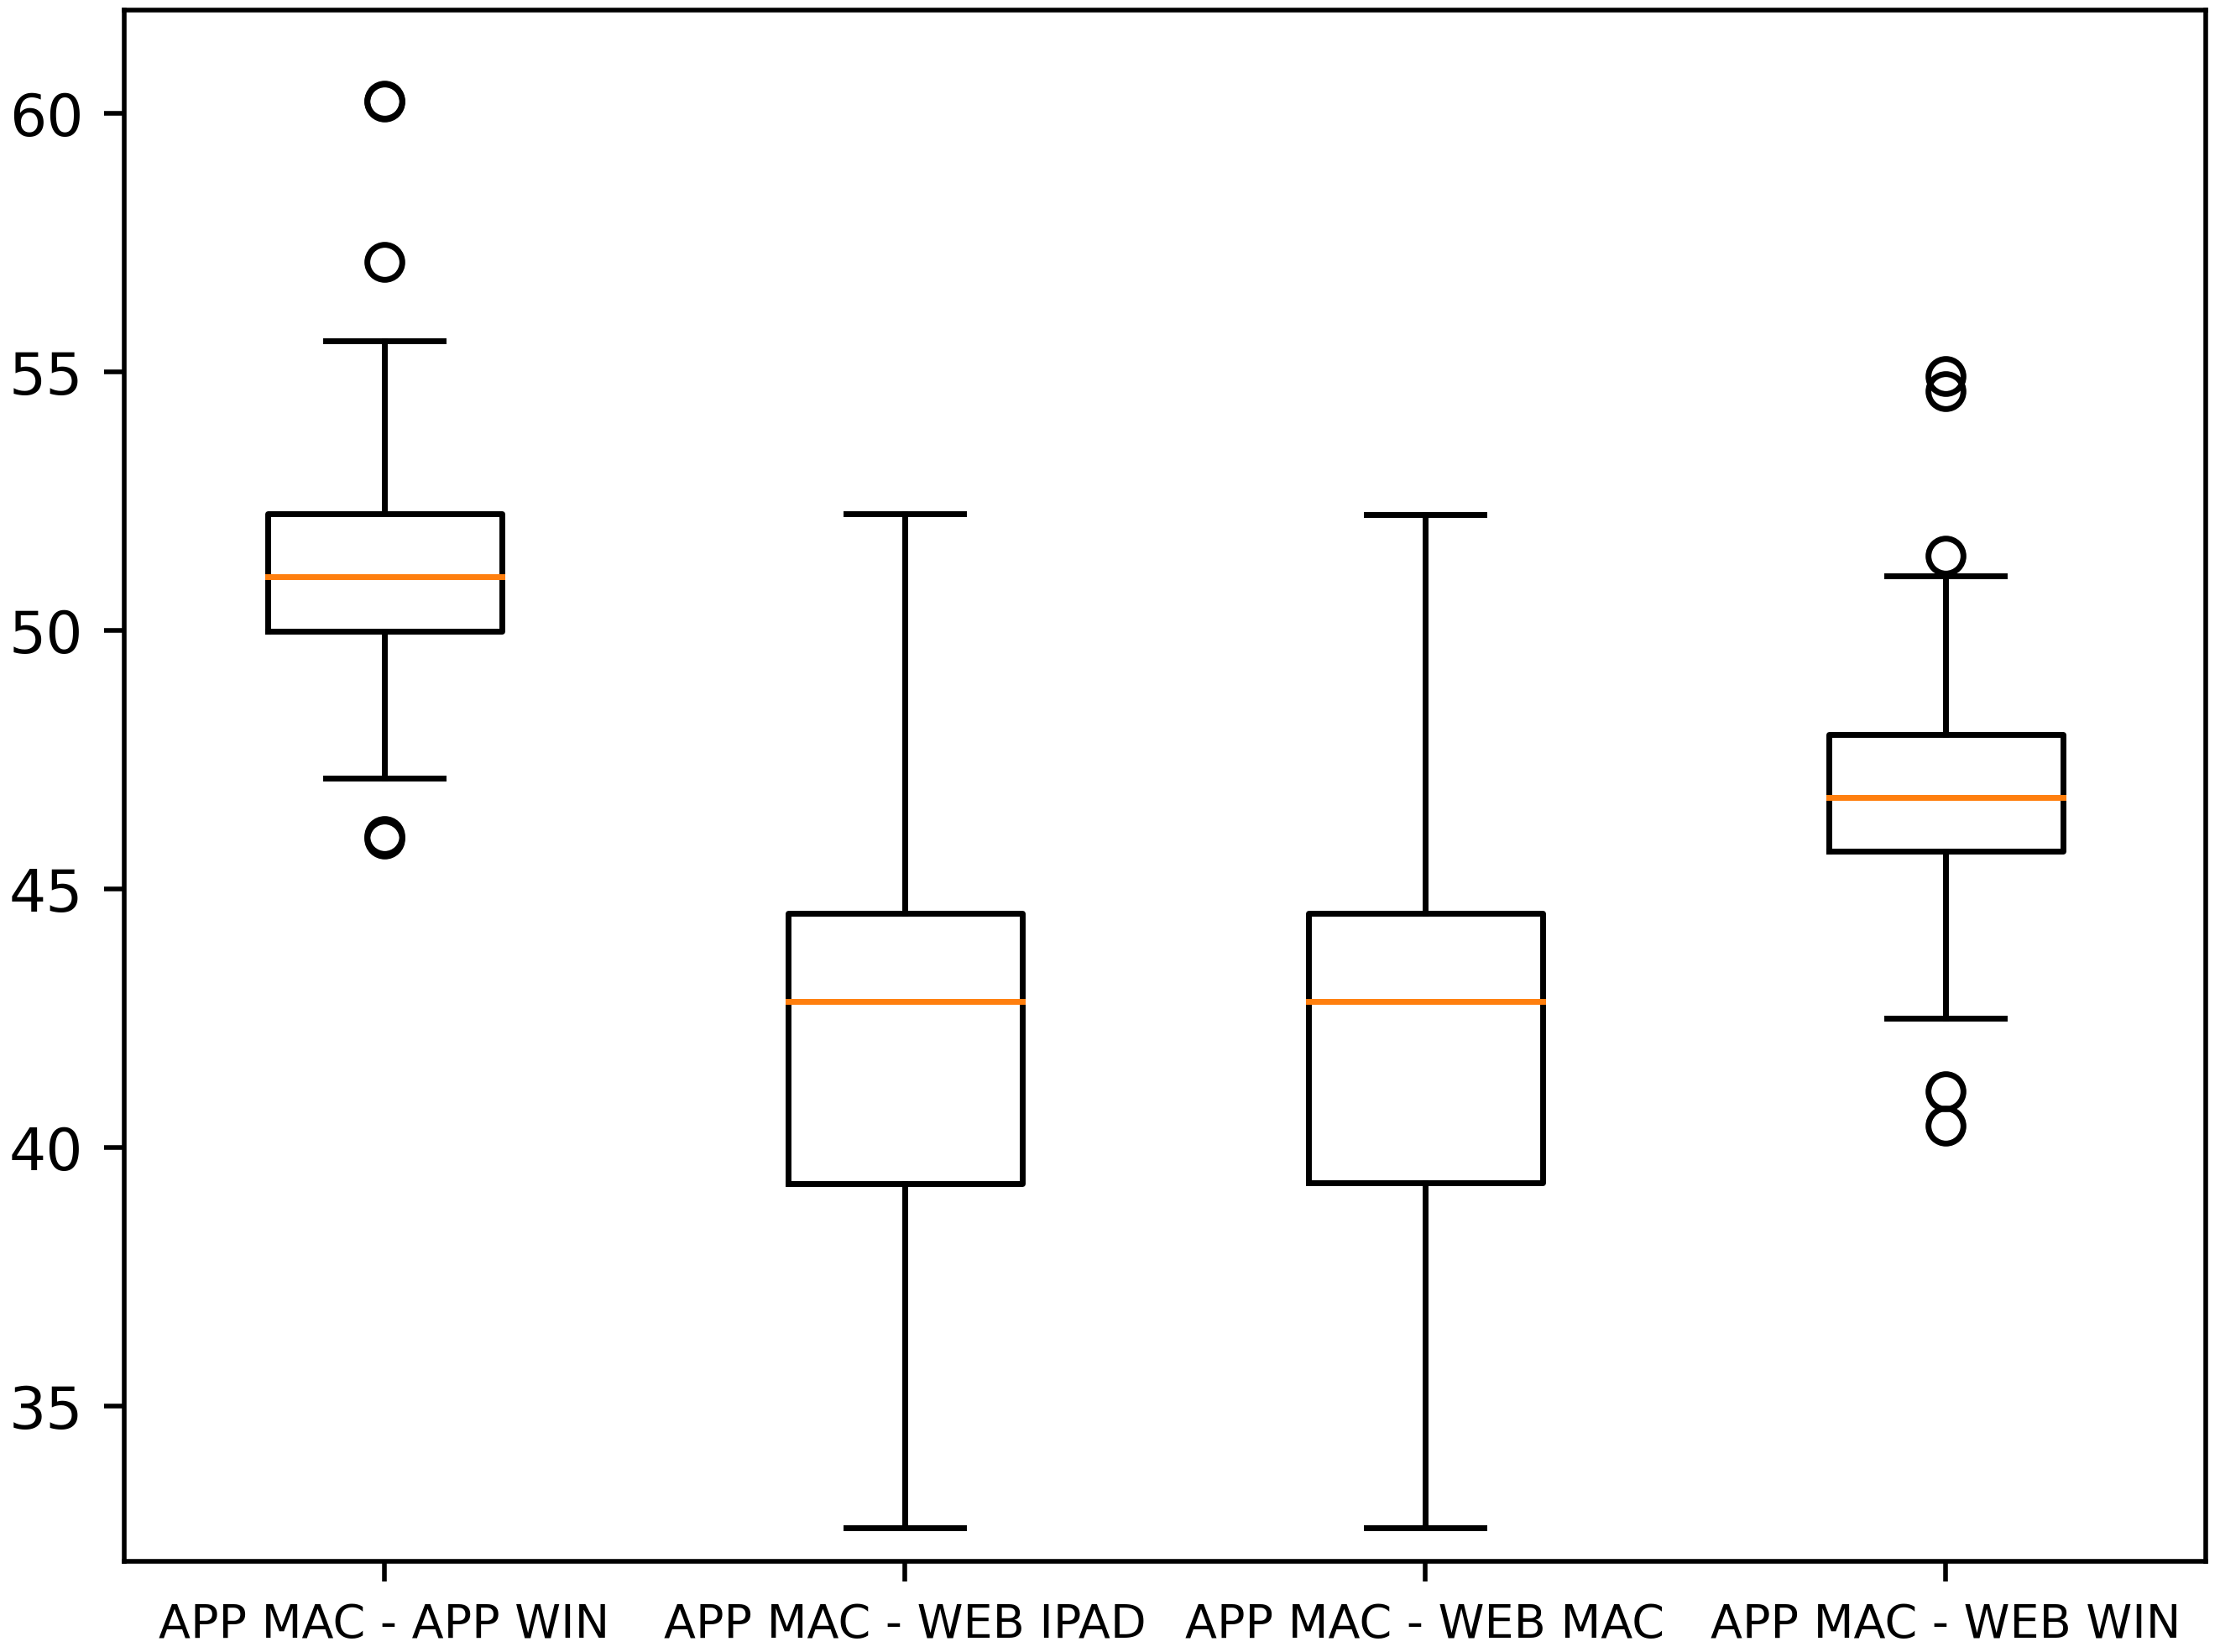
\includegraphics[width=8cm, height=8cm, keepaspectratio]{Immagini/PSNR/Immagine1.png}\hspace{1em}
    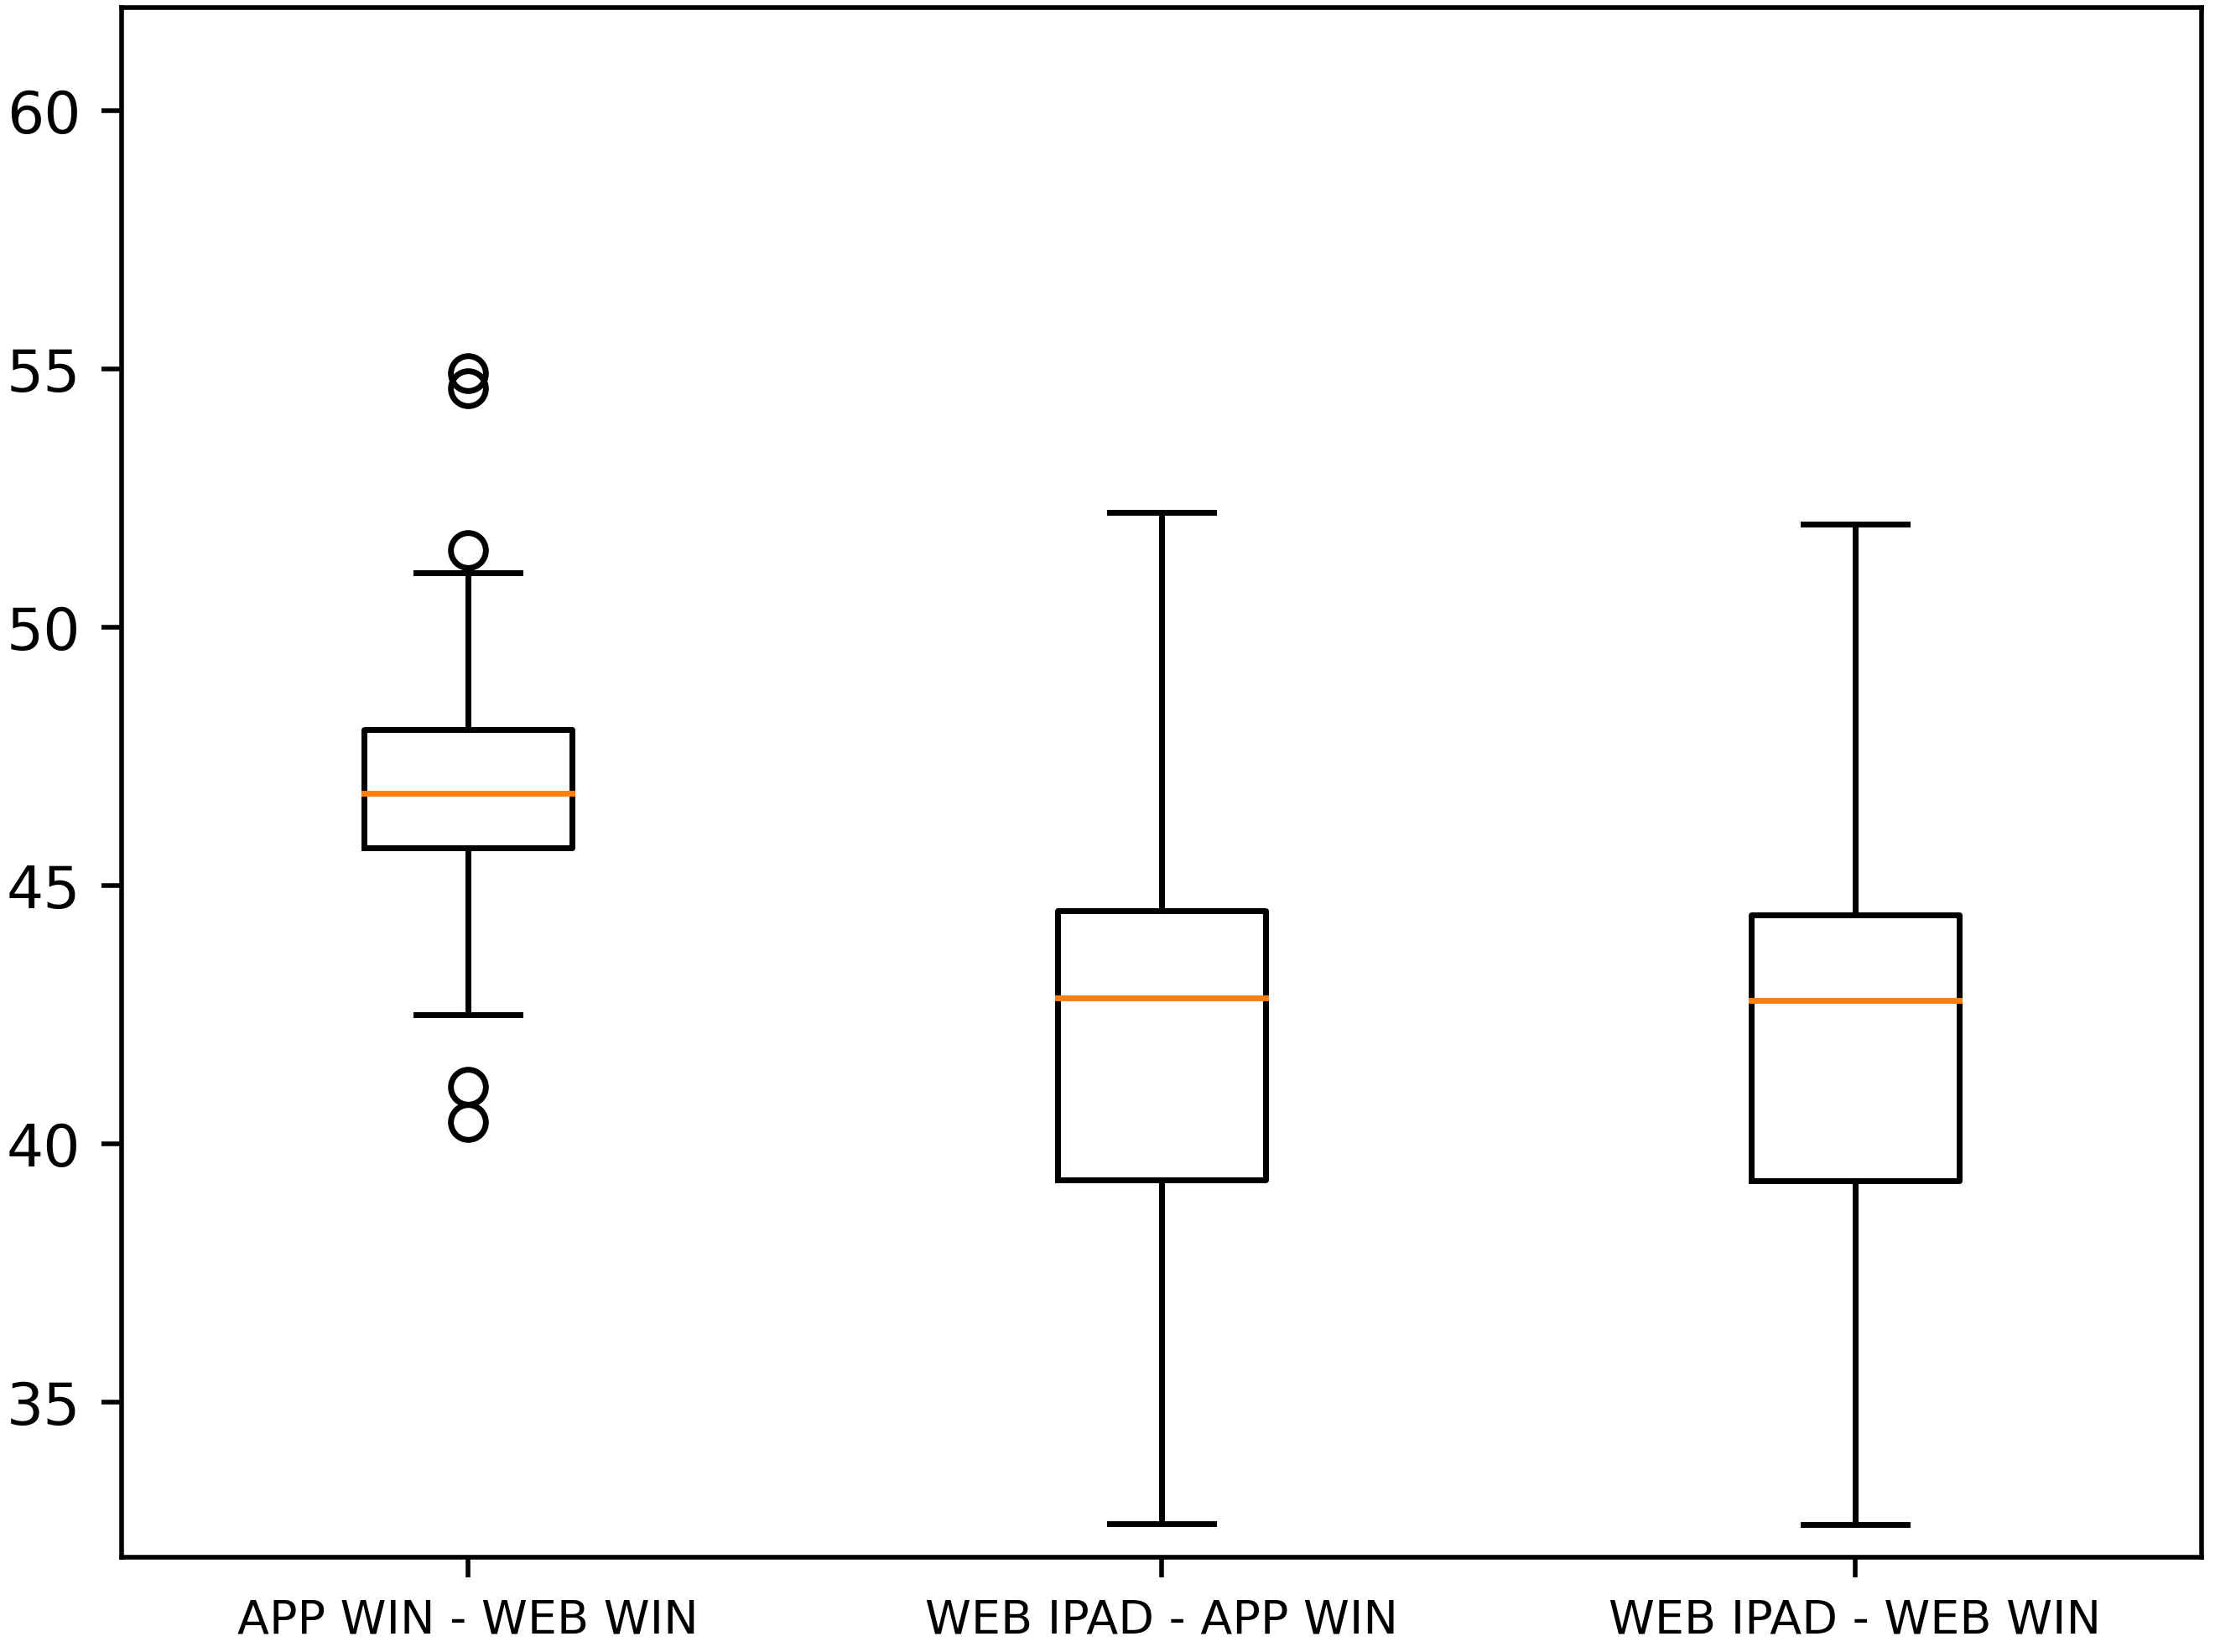
\includegraphics[width=8cm, height=8cm, keepaspectratio]{Immagini/PSNR/Immagine2.png}\\\vspace{1em}
    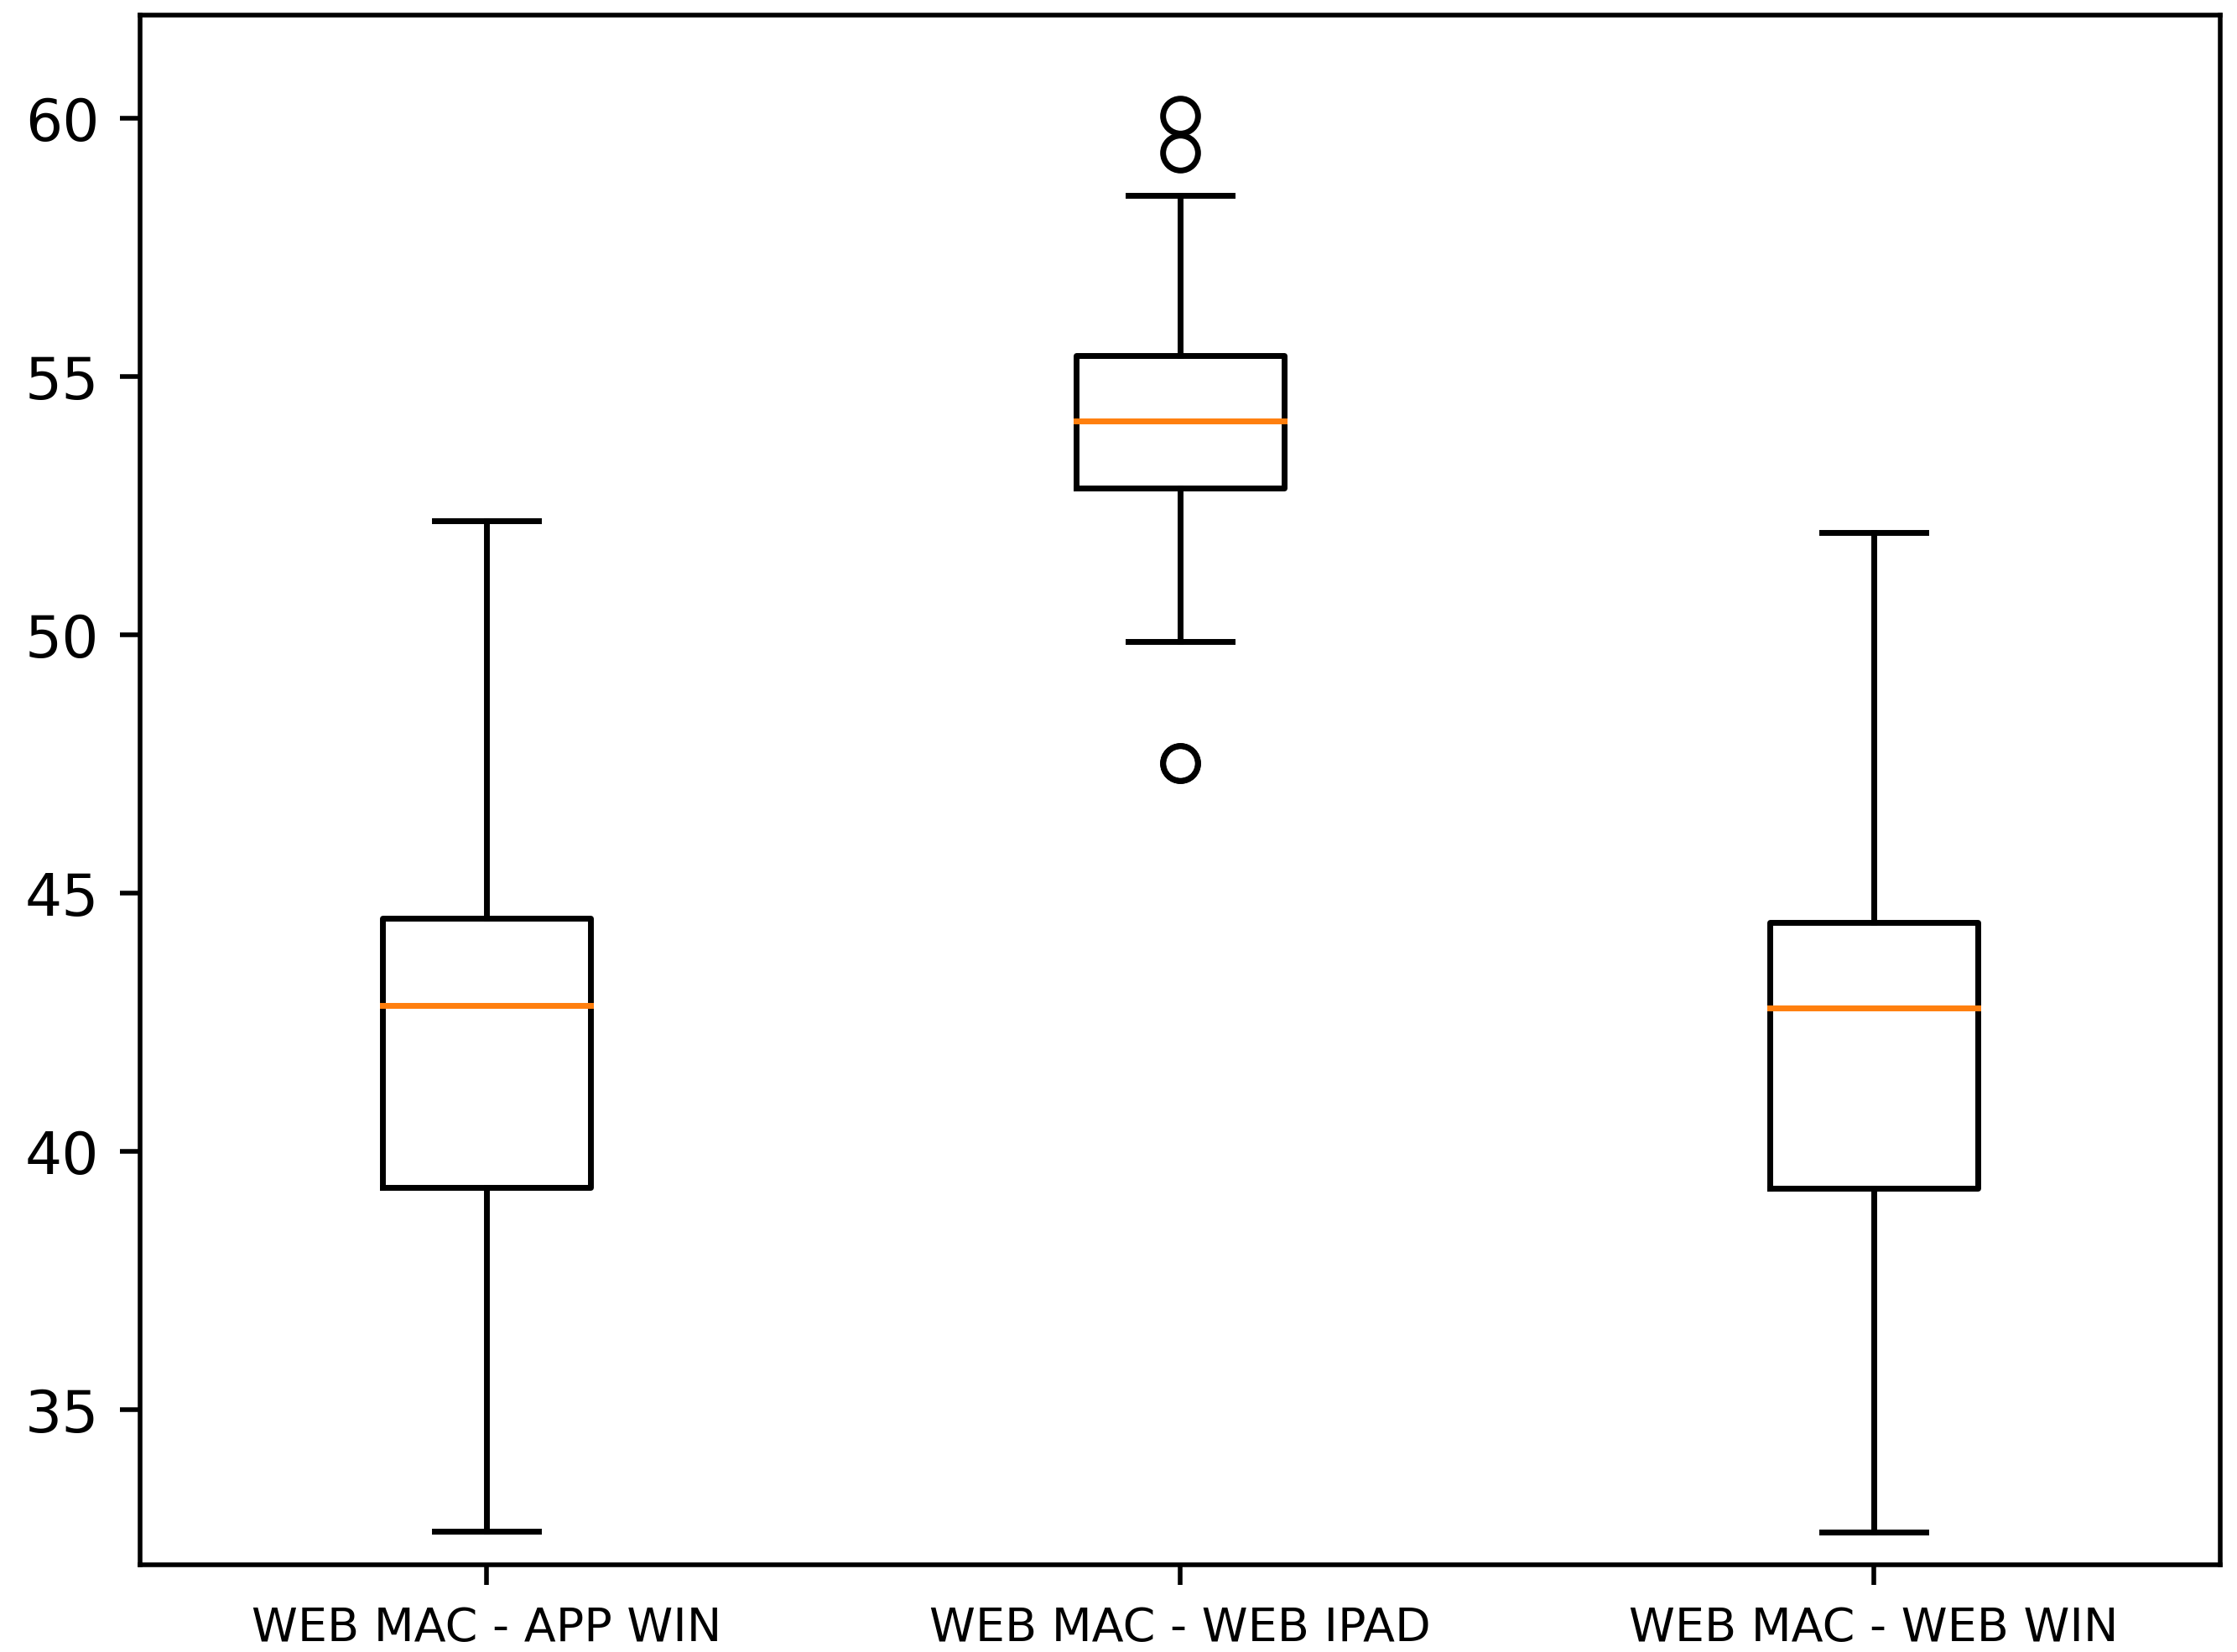
\includegraphics[width=8cm, height=8cm, keepaspectratio]{Immagini/PSNR/Immagine3.png}
    \captionof{figure}{\textit{Boxplot} ricavati dal calcolo del PSNR.}
    \label{fig:psnr_results}
\endgroup

\section{Analisi feature}
\label{sec:feaure_results}
I primi due diagrammi in Fig.~\ref{fig:all_isomap} mostrano la visualizzazione delle \textit{feature} con uno zoom sul cluster centrale in posizione $(0,0)$. A livello macroscopico, i punti che appartengono alla classe \textit{IPHONE} sono ben separati e vanno a formare un insieme di punti distinto dimostrando un'eterogeneità delle \textit{feature} ottenute durante la fase di estrazione. Osservando in dettaglio grazie allo zoom, notiamo che la maggior parte delle classi presenta cluster che sono abbastanza definiti (es., \textit{WEB-WIN}), con due eccezioni: i punti appartenenti alla classe \textit{APP-MAC} sono perfettamente sovrapposti a \textit{APP-WIN} mentre quelli etichettati come \textit{WEB-IPAD} si trovano nella stessa posizione di \textit{WEB-MAC}. Ciò significa che i vettori di \textit{feature} rappresentativi delle immagini hanno gli stessi valori e non possono essere separati. Per questo motivo sono state create due nuove classi:

\begin{itemize}
    \item \textit{APP-DESKTOP}: ottenuta dalla fusione di \textit{APP-MAC} con \textit{APP-WIN}, contiene le immagini condivise tramite l'applicazione desktop di WhatsApp per MacOS e Windows 10;
    
    \item \textit{WEB-SAFARI}: ottenuta dall'unione di \textit{WEB-MAC} con \textit{WEB-IPAD}, include tutte le immagini condivise con il browser Safari tramite tablet e computer.
\end{itemize}

La lista finale delle classi che verranno utilizzate d'ora in poi è quindi composta da: \textit{ANDROID}, \textit{APP-DESKTOP}, \textit{IPHONE}, \textit{WEB-SAFARI} e \textit{WEB-WIN}. A seguito di questa operazione abbiamo eseguito nuovamente la visualizzazione Isomap e i risultati ottenuti sono rappresentati negli ultimi due grafici in Fig.~\ref{fig:all_isomap}. Rispetto a prima, il grado di separazione dei cluster di punti è elevato, fattore che indica una diversità più marcata dei valori delle \textit{feature}. Da ultimo, è stata effettuata la visualizzazione anche per i singoli \textit{quality factor} e, anche se non riportati, i dati ottenuti sono conformi a quanto mostrato finora.\\\\

% \begin{figure}[h!]
%     \centering
%     \subfloat[][]{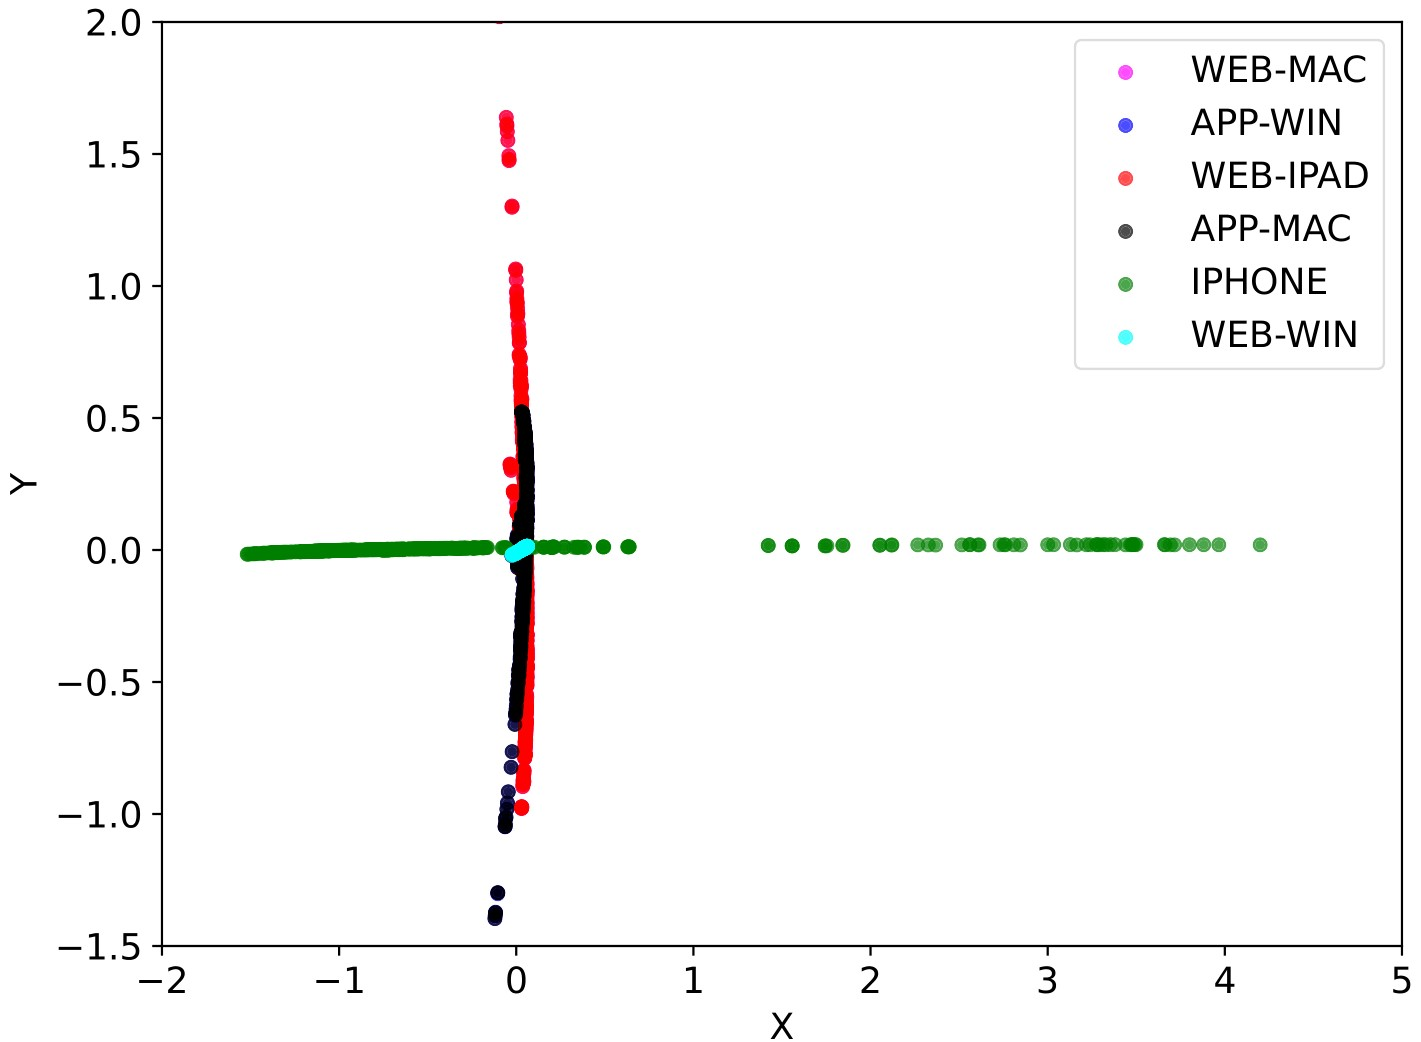
\includegraphics[width=8.5cm, height=8.5cm, keepaspectratio]{Immagini/Isomap/isomap_sep_class.jpg}\label{fig:isomap_sep_class}}
%     \subfloat[][]{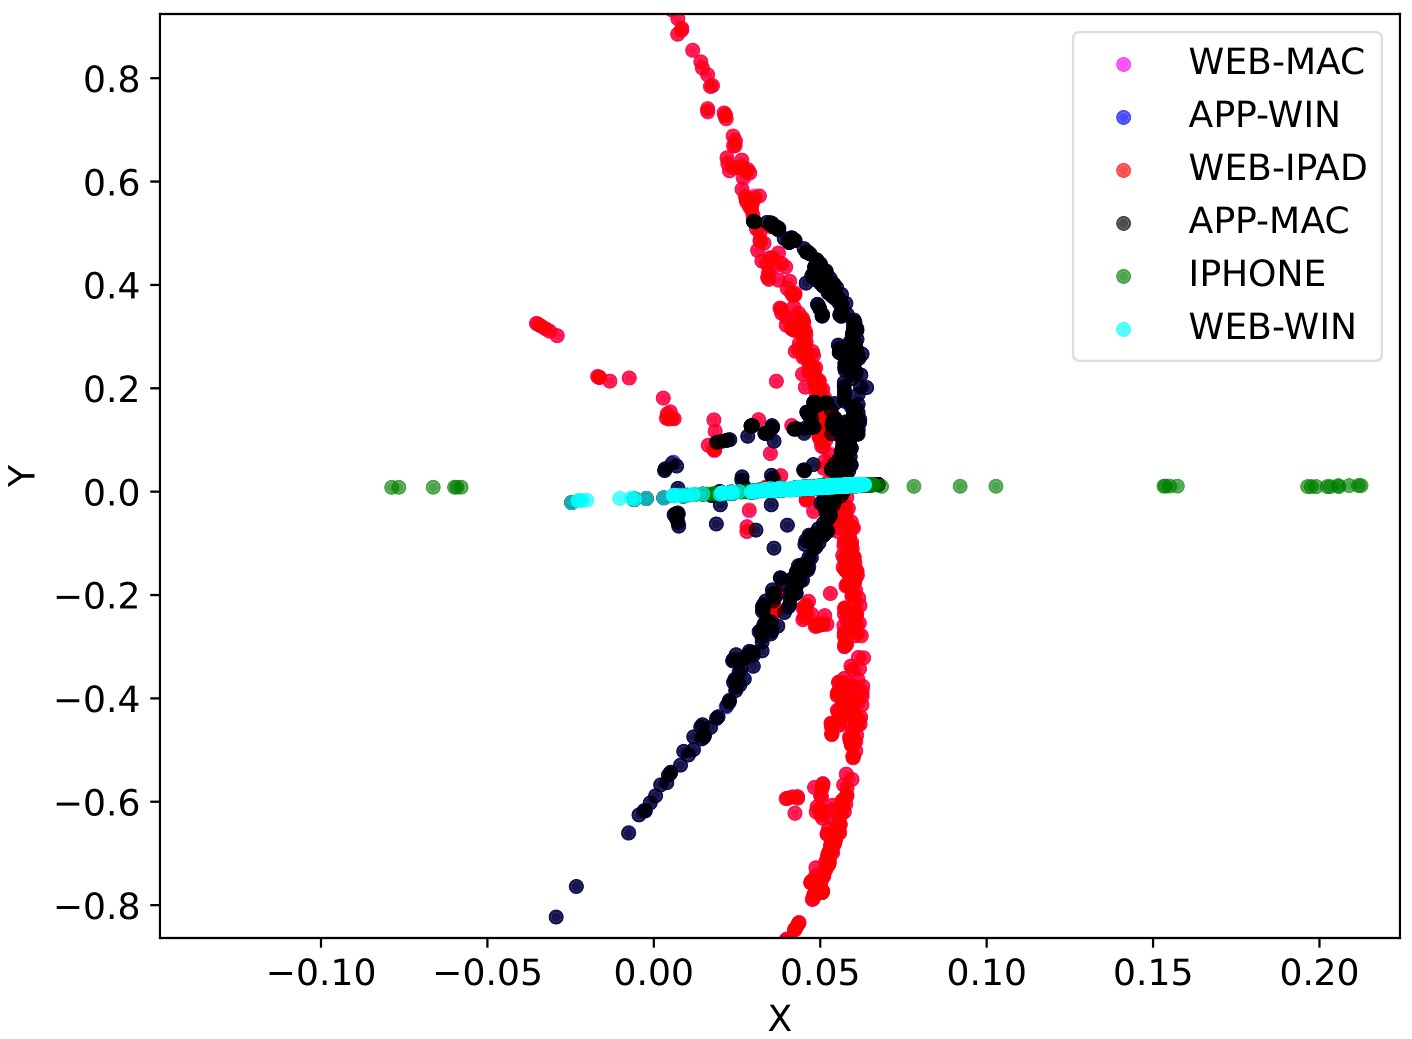
\includegraphics[width=8.5cm, height=8.5cm, keepaspectratio]{Immagini/Isomap/zoom_isomap_sep_class.jpg}\label{fig:isomap_sep_class_zoom}}\\\vspace{1em}
%     \subfloat[][]{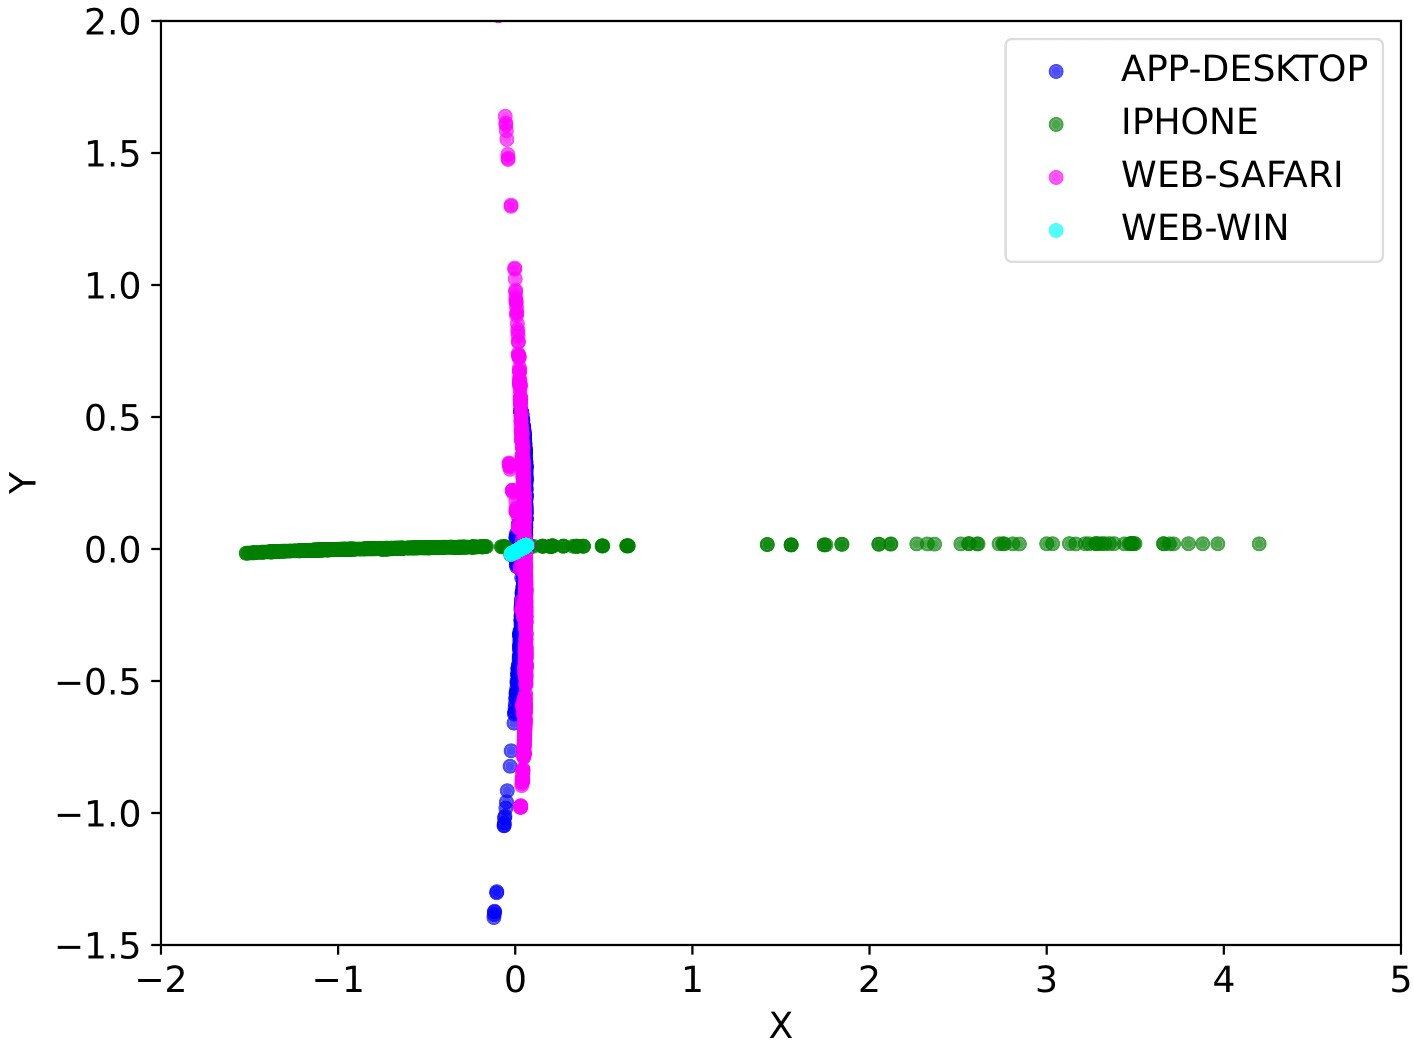
\includegraphics[width=8.5cm, height=8.5cm, keepaspectratio]{Immagini/Isomap/isomap.jpg}\label{fig:isomap}}
%     \subfloat[][]{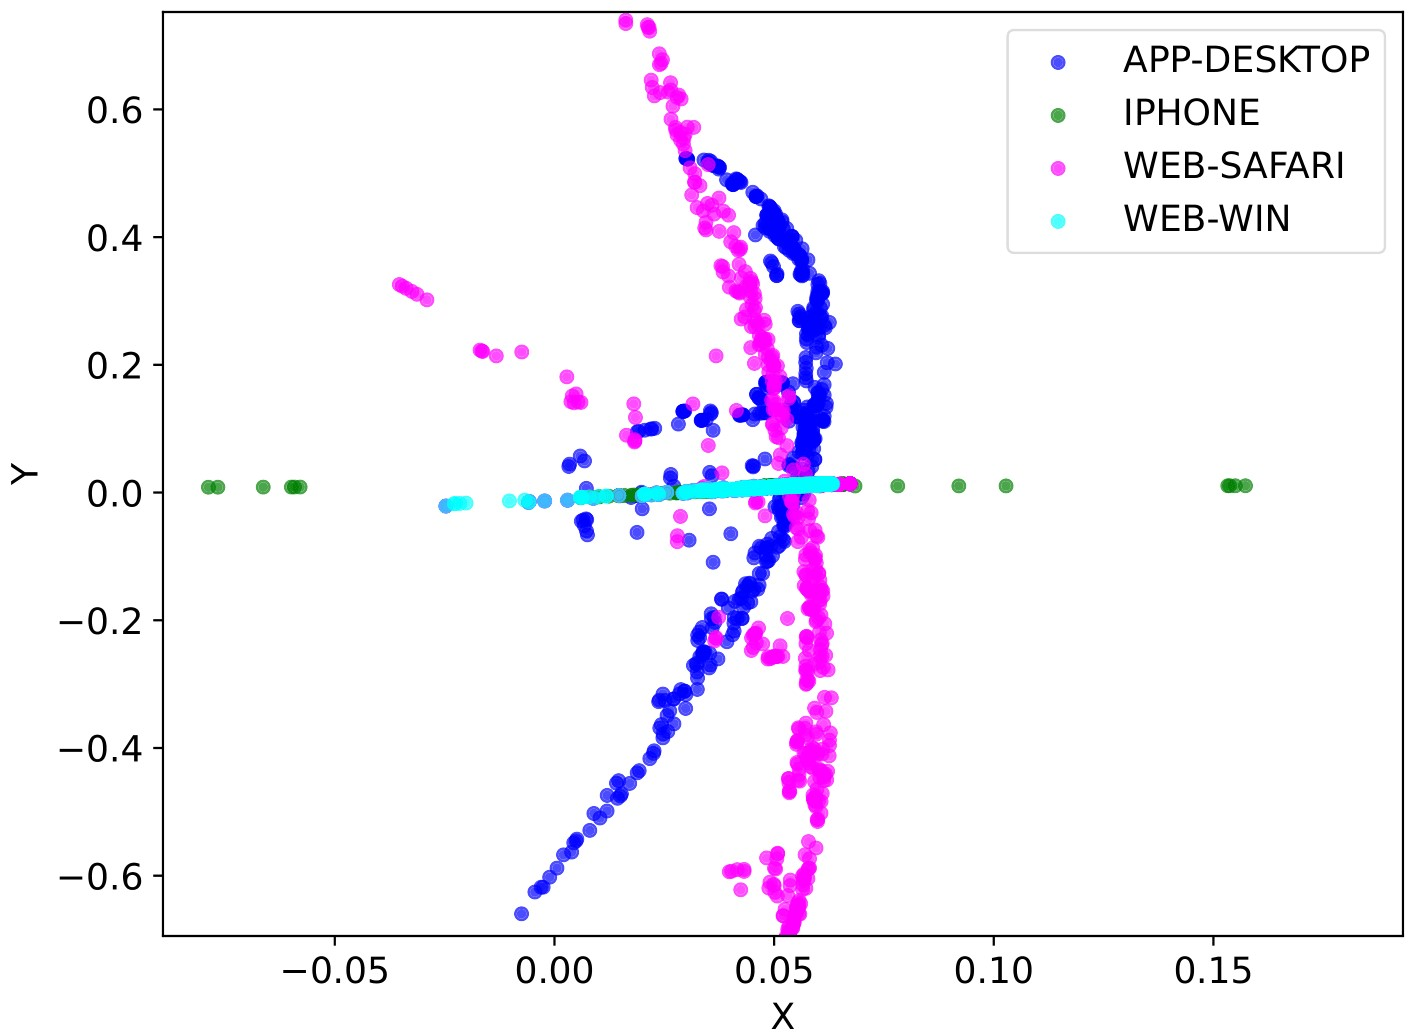
\includegraphics[width=8.5cm, height=8.5cm, keepaspectratio]{Immagini/Isomap/zoom_isomap.jpg}\label{fig:isomap_zoom}}
%     \caption{Rappresentazione Isomap dei vettori di \textit{feature} estratti dalle immagini di SHADE, con una vista complessiva (a, c) e un ingrandimento del cluster vicino all'origine (b, d), sia per le classi separate che dopo la fusione.}
% \end{figure}

\begingroup
    \centering
    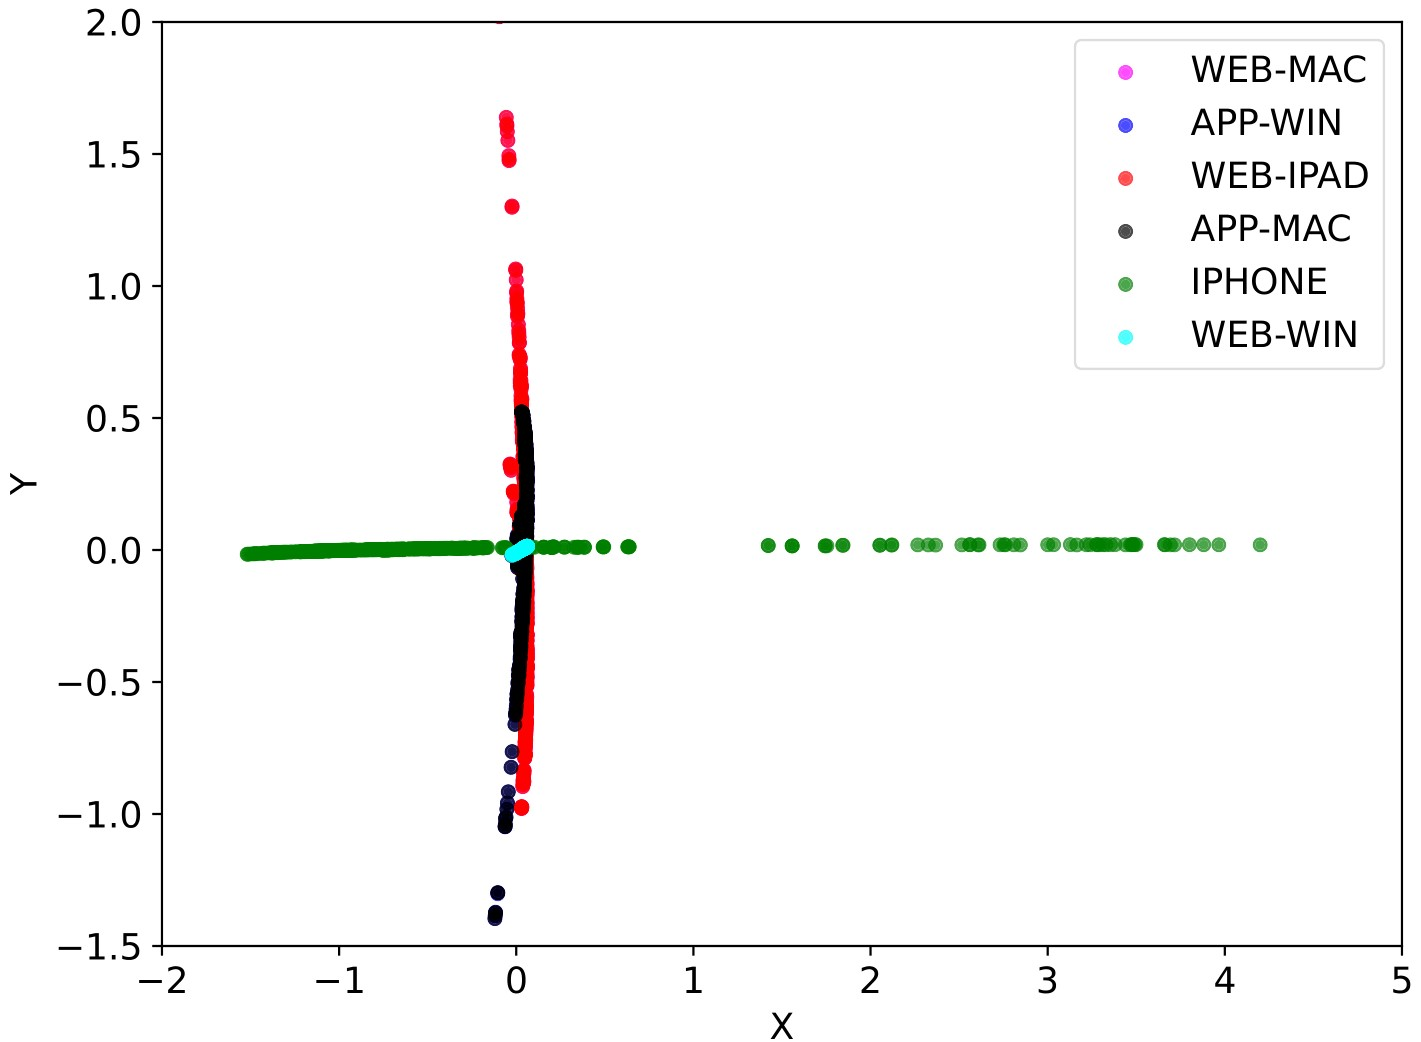
\includegraphics[width=8.5cm, height=8.5cm, keepaspectratio]{Immagini/Isomap/isomap_sep_class.jpg}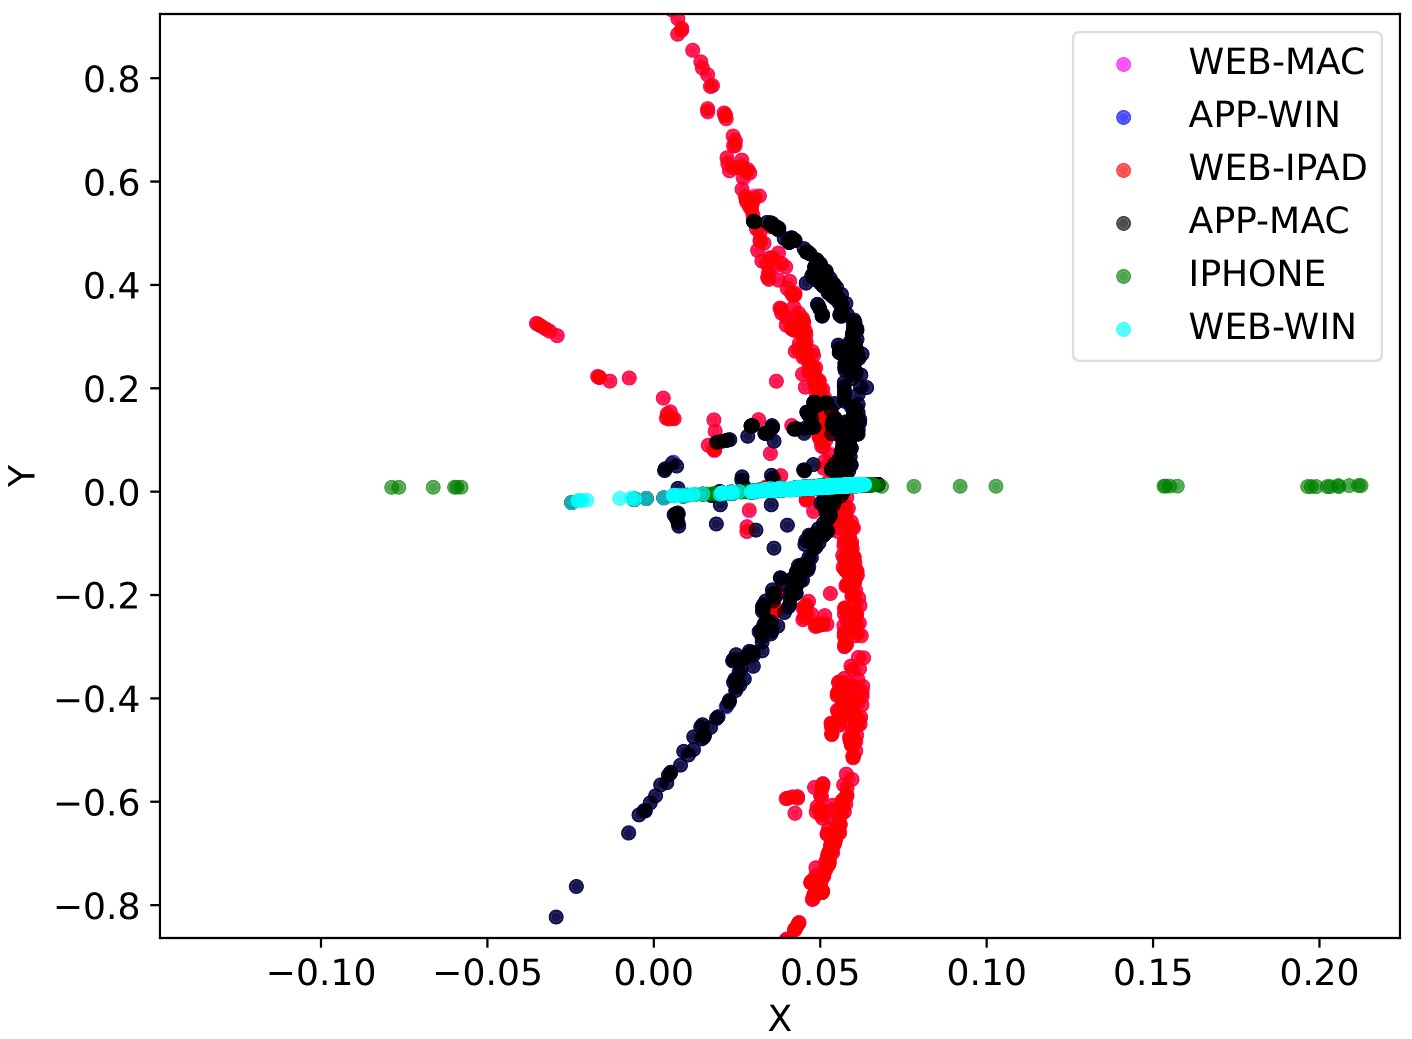
\includegraphics[width=8.5cm, height=8.5cm, keepaspectratio]{Immagini/Isomap/zoom_isomap_sep_class.jpg}\\\vspace{1em}
    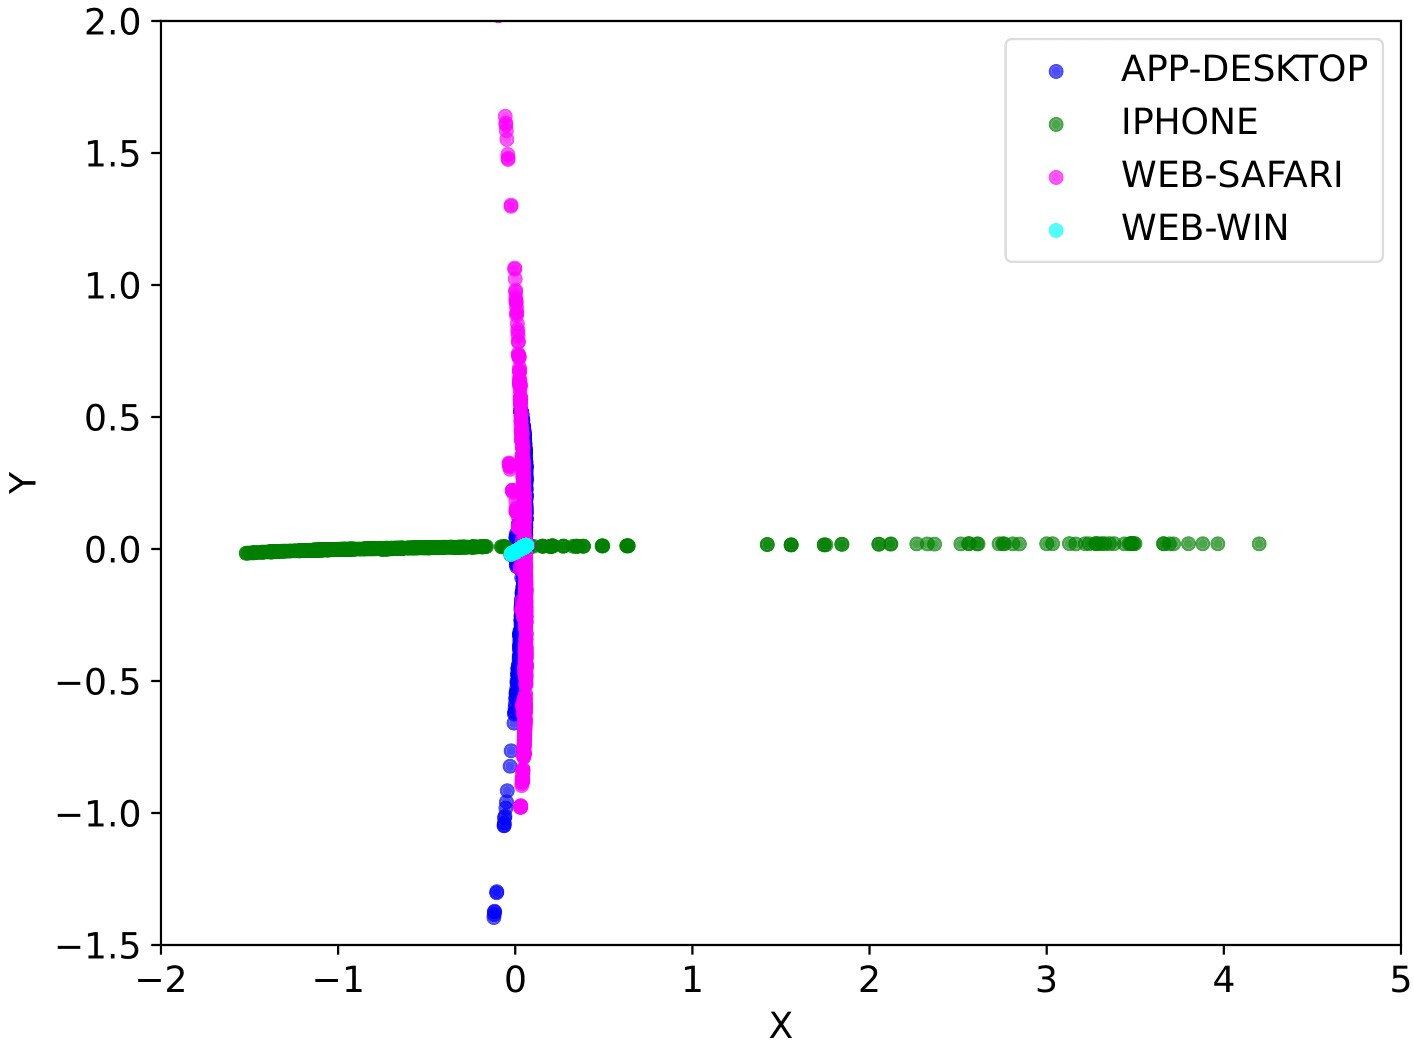
\includegraphics[width=8.5cm, height=8.5cm, keepaspectratio]{Immagini/Isomap/isomap.jpg}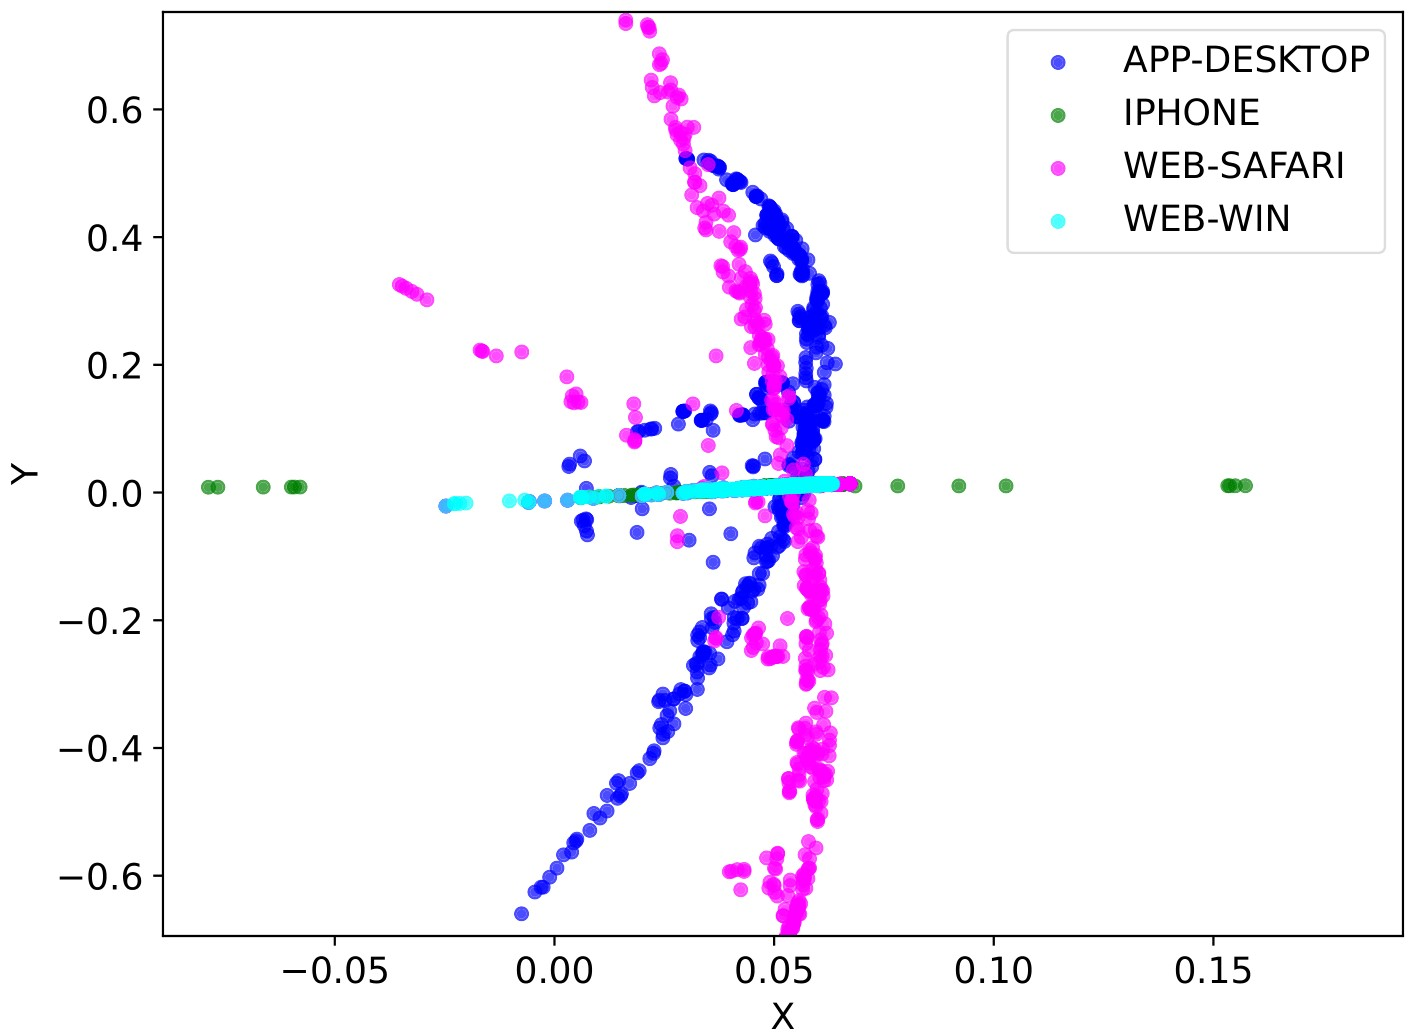
\includegraphics[width=8.5cm, height=8.5cm, keepaspectratio]{Immagini/Isomap/zoom_isomap.jpg}
    \captionof{figure}{Rappresentazione Isomap dei vettori di \textit{feature} estratti dalle immagini di SHADE, con una vista complessiva e un ingrandimento del cluster vicino all'origine, sia per le classi separate che dopo la fusione.}
    \label{fig:all_isomap}
\endgroup

\section{Classificazione}
\label{sec:classification_results}
Terminiamo la presentazione dei risultati mostrando le \textit{confusion matrix} (Fig.~\ref{fig:class}) ottenute dalla classificazione. Ogni cella $(i,j)$ di queste tabelle, con $i$ come riga e $j$ come colonna, contiene il numero di immagini predette con classe $j$ rispetto al metodo di condivisione $i$. Il numero ottenuto è stato poi normalizzato in modo da essere compreso tra 0 e 1. Il dato più rilevante riscontrato è che la classe \textit{IPHONE} viene identificata correttamente nel 100\% dei casi, confermando quanto era emerso dalla visualizzazione Isomap. Per quanto riguarda le rimanenti classi, le performance ottenute sono soddisfacenti con valori di accuratezza che variano tra il 69\% e il 73\% nel caso di \textit{random forest} e tra il 72\% e il 78\% nel caso di \textit{support vector machine}. La seguente tabella mostra per ogni classe considerata quella con più falsi positivi.

\begin{center}
    \begin{tabular}{llll}
    \hline
    \\[-1em]
    \textbf{metodo} & \textbf{classe} & \textbf{classe con più falsi positivi} & \textbf{N. occorrenze} \\[-1em]\\
    \hline
    \\[-1em]
    \multirow{5}{4em}{\textbf{RF}} & \textit{APP-DESKTOP} & \textit{ANDROID} & 234 \\[-1em]\\
    & \textit{IPHONE} & - & - \\[-1em]\\
    & \textit{WEB-SAFARI} & \textit{ANDROID} & 252 \\[-1em]\\
    & \textit{WEB-WIN} & \textit{ANDROID} & 108 \\[-1em]\\
    & \textit{ANDROID} & \textit{APP-DESKTOP} & 117 \\[-1em]\\
    \hline
    \\[-1em]
    \multirow{5}{4em}{\textbf{SVM}} & \textit{APP-DESKTOP} & \textit{WEB-SAFARI} & 234 \\[-1em]\\
    & \textit{IPHONE} & - & - \\[-1em]\\
    & \textit{WEB-SAFARI} & \textit{APP-DESKTOP } & 180 \\[-1em]\\
    & \textit{WEB-WIN} & \textit{WEB-SAFARI} & 99 \\[-1em]\\
    & \textit{ANDROID} & \textit{WEB-SAFARI} & 108 \\[-1em]\\
    \hline
    \end{tabular}
\end{center}

Nonostante le performance non raggiungano il livello di \textit{IPHONE}, le classi analizzate sono comunque ben separabili e possono essere identificate abbastanza facilmente. La classificazione delle immagini in base al \textit{quality factor} (Fig.~\ref{fig:class_QF_RF},~\ref{fig:class_QF_SVM}) ha dato risultati simili sia per RF che per SVM. Abbiamo notato però che in quest'ultimo caso il livello di accuratezza è minore per alcune classi ma più elevato per altre.\\

\begingroup
    \centering
    \subfloat[][]{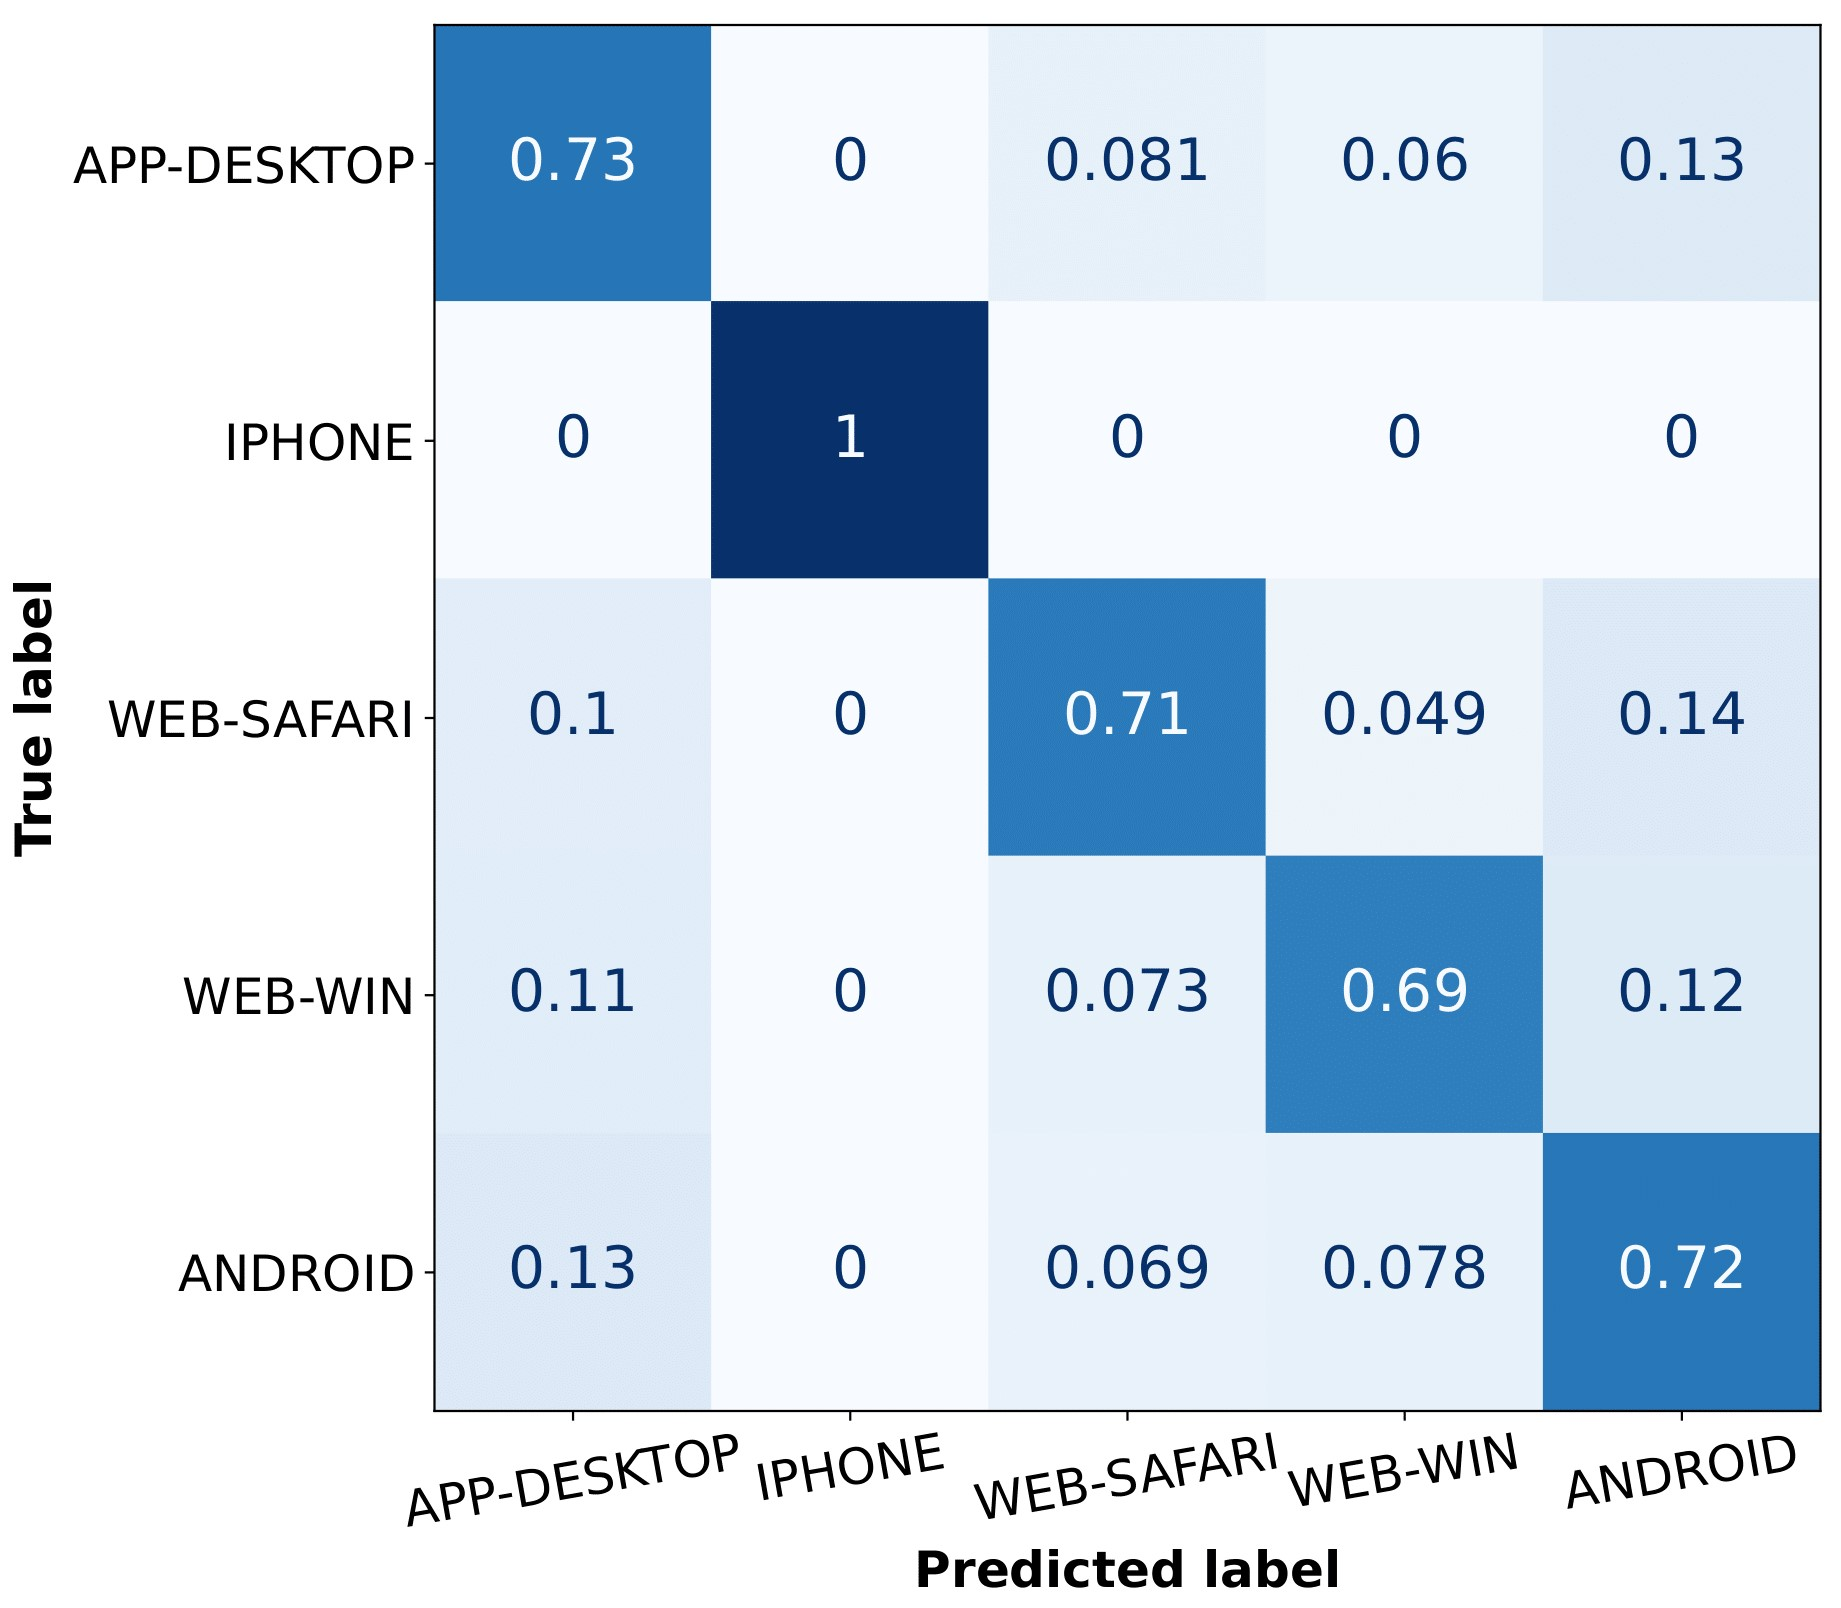
\includegraphics[width=8cm, height=8cm, keepaspectratio]{Immagini/Classificazione/confusion_matrix_RF.jpg}}\ \ \ \ \
    \subfloat[][]{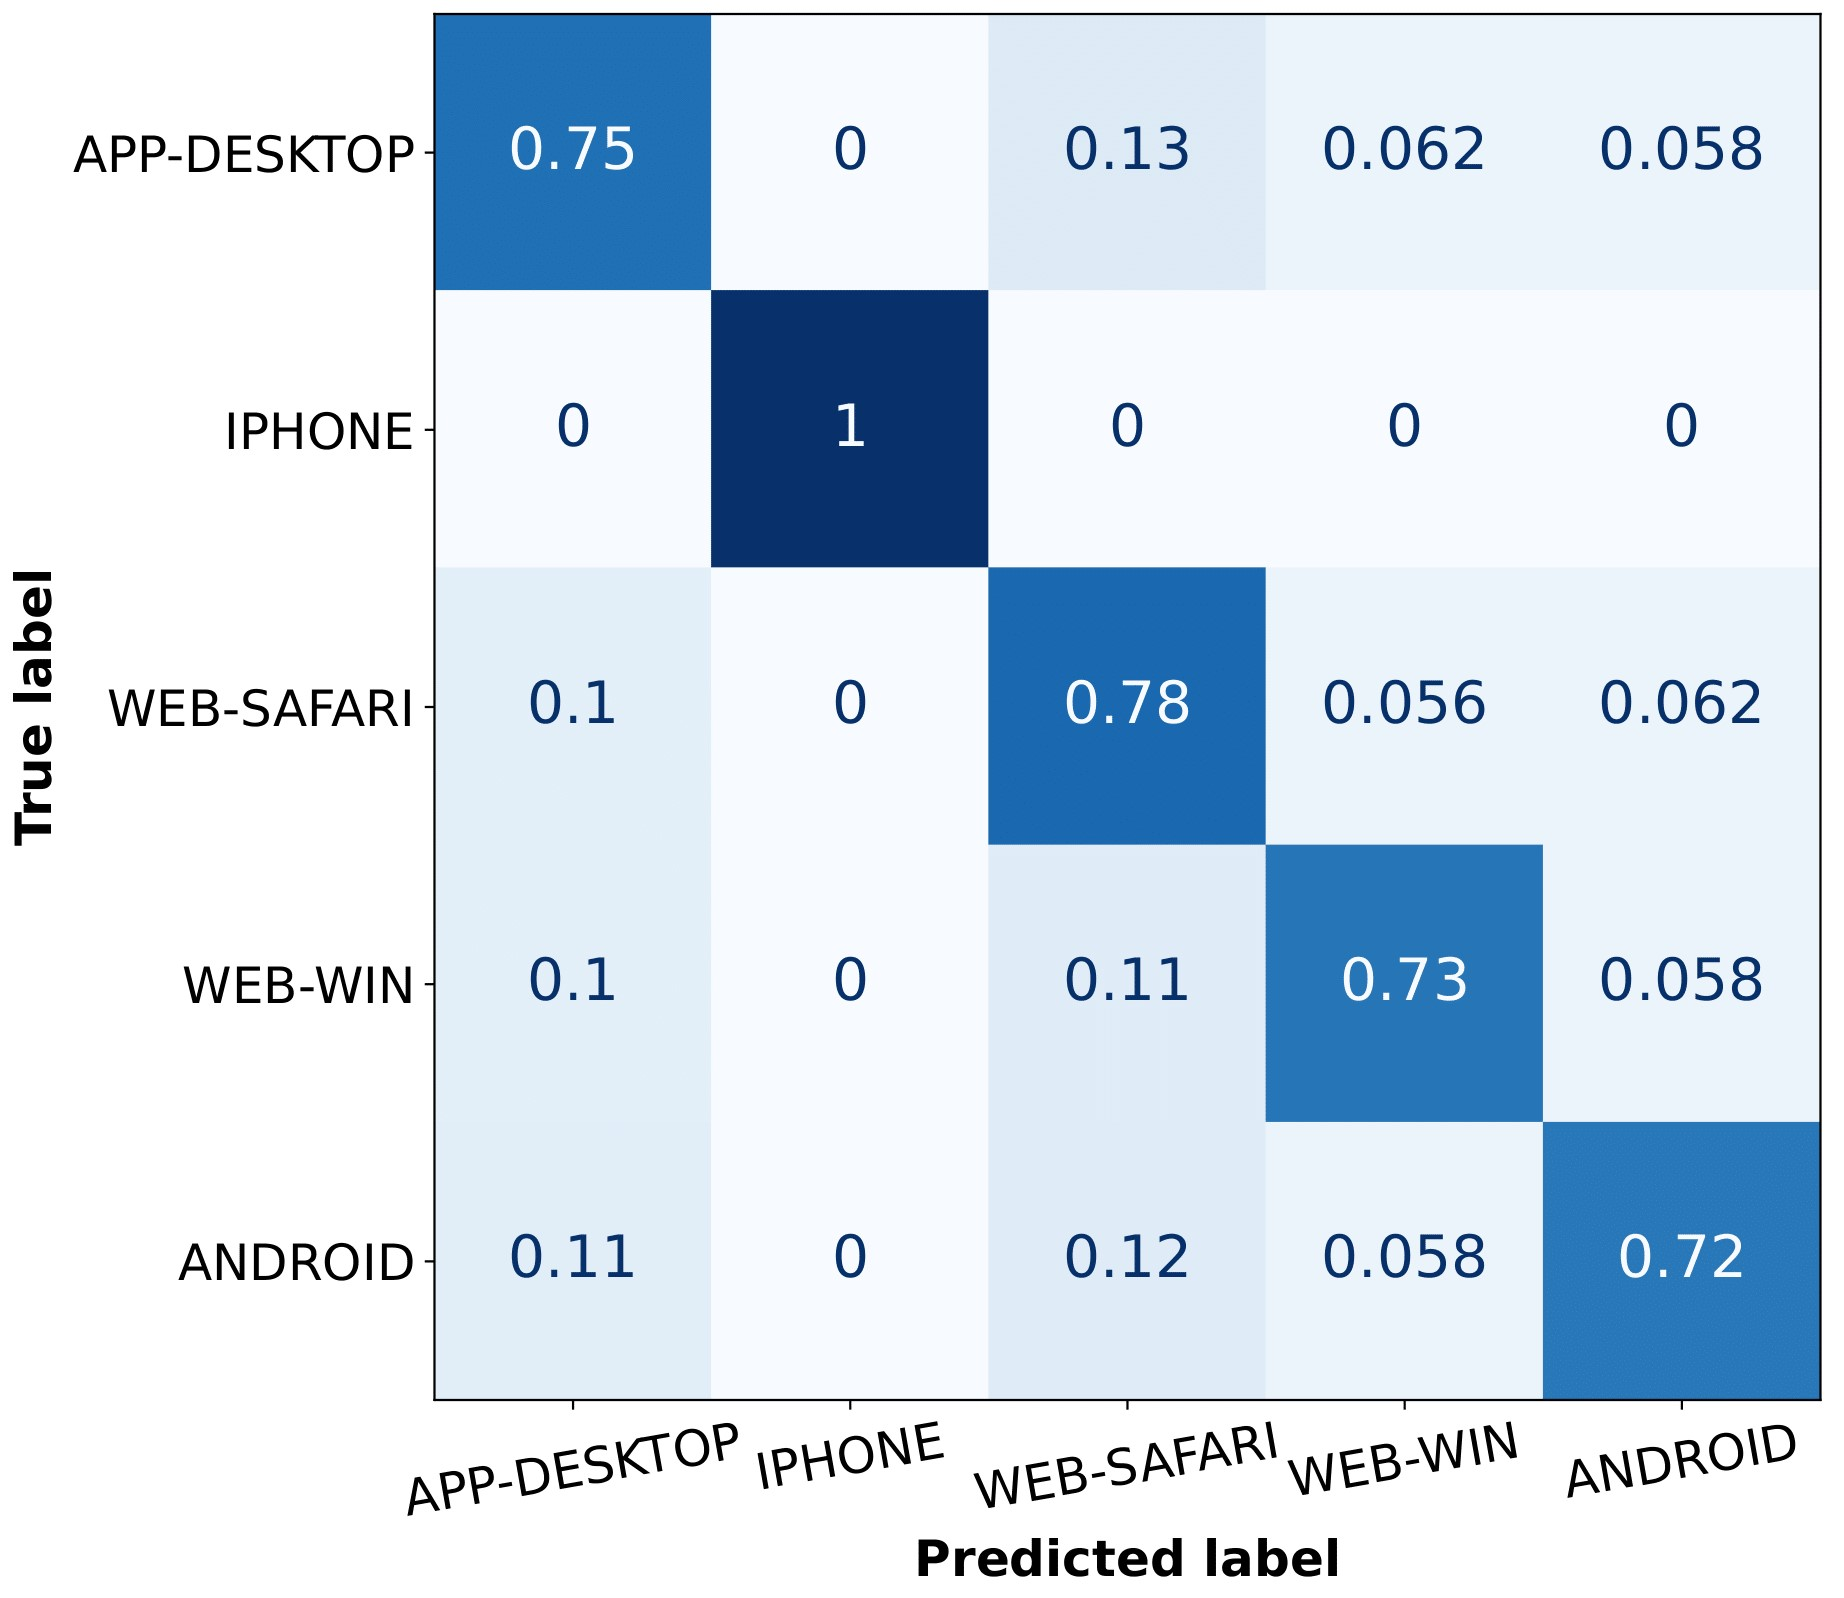
\includegraphics[width=8cm, height=8cm, keepaspectratio]{Immagini/Classificazione/confusion_matrix_SVM.jpg}}\\  
    \captionof{figure}{\textit{Confusion matrix} per la classificazione delle immagini di SHADE con (a) \textit{random forest} e (b) \textit{support vector machine}.}
    \label{fig:class}
\endgroup

\vspace{1em}

\begingroup
    \centering
    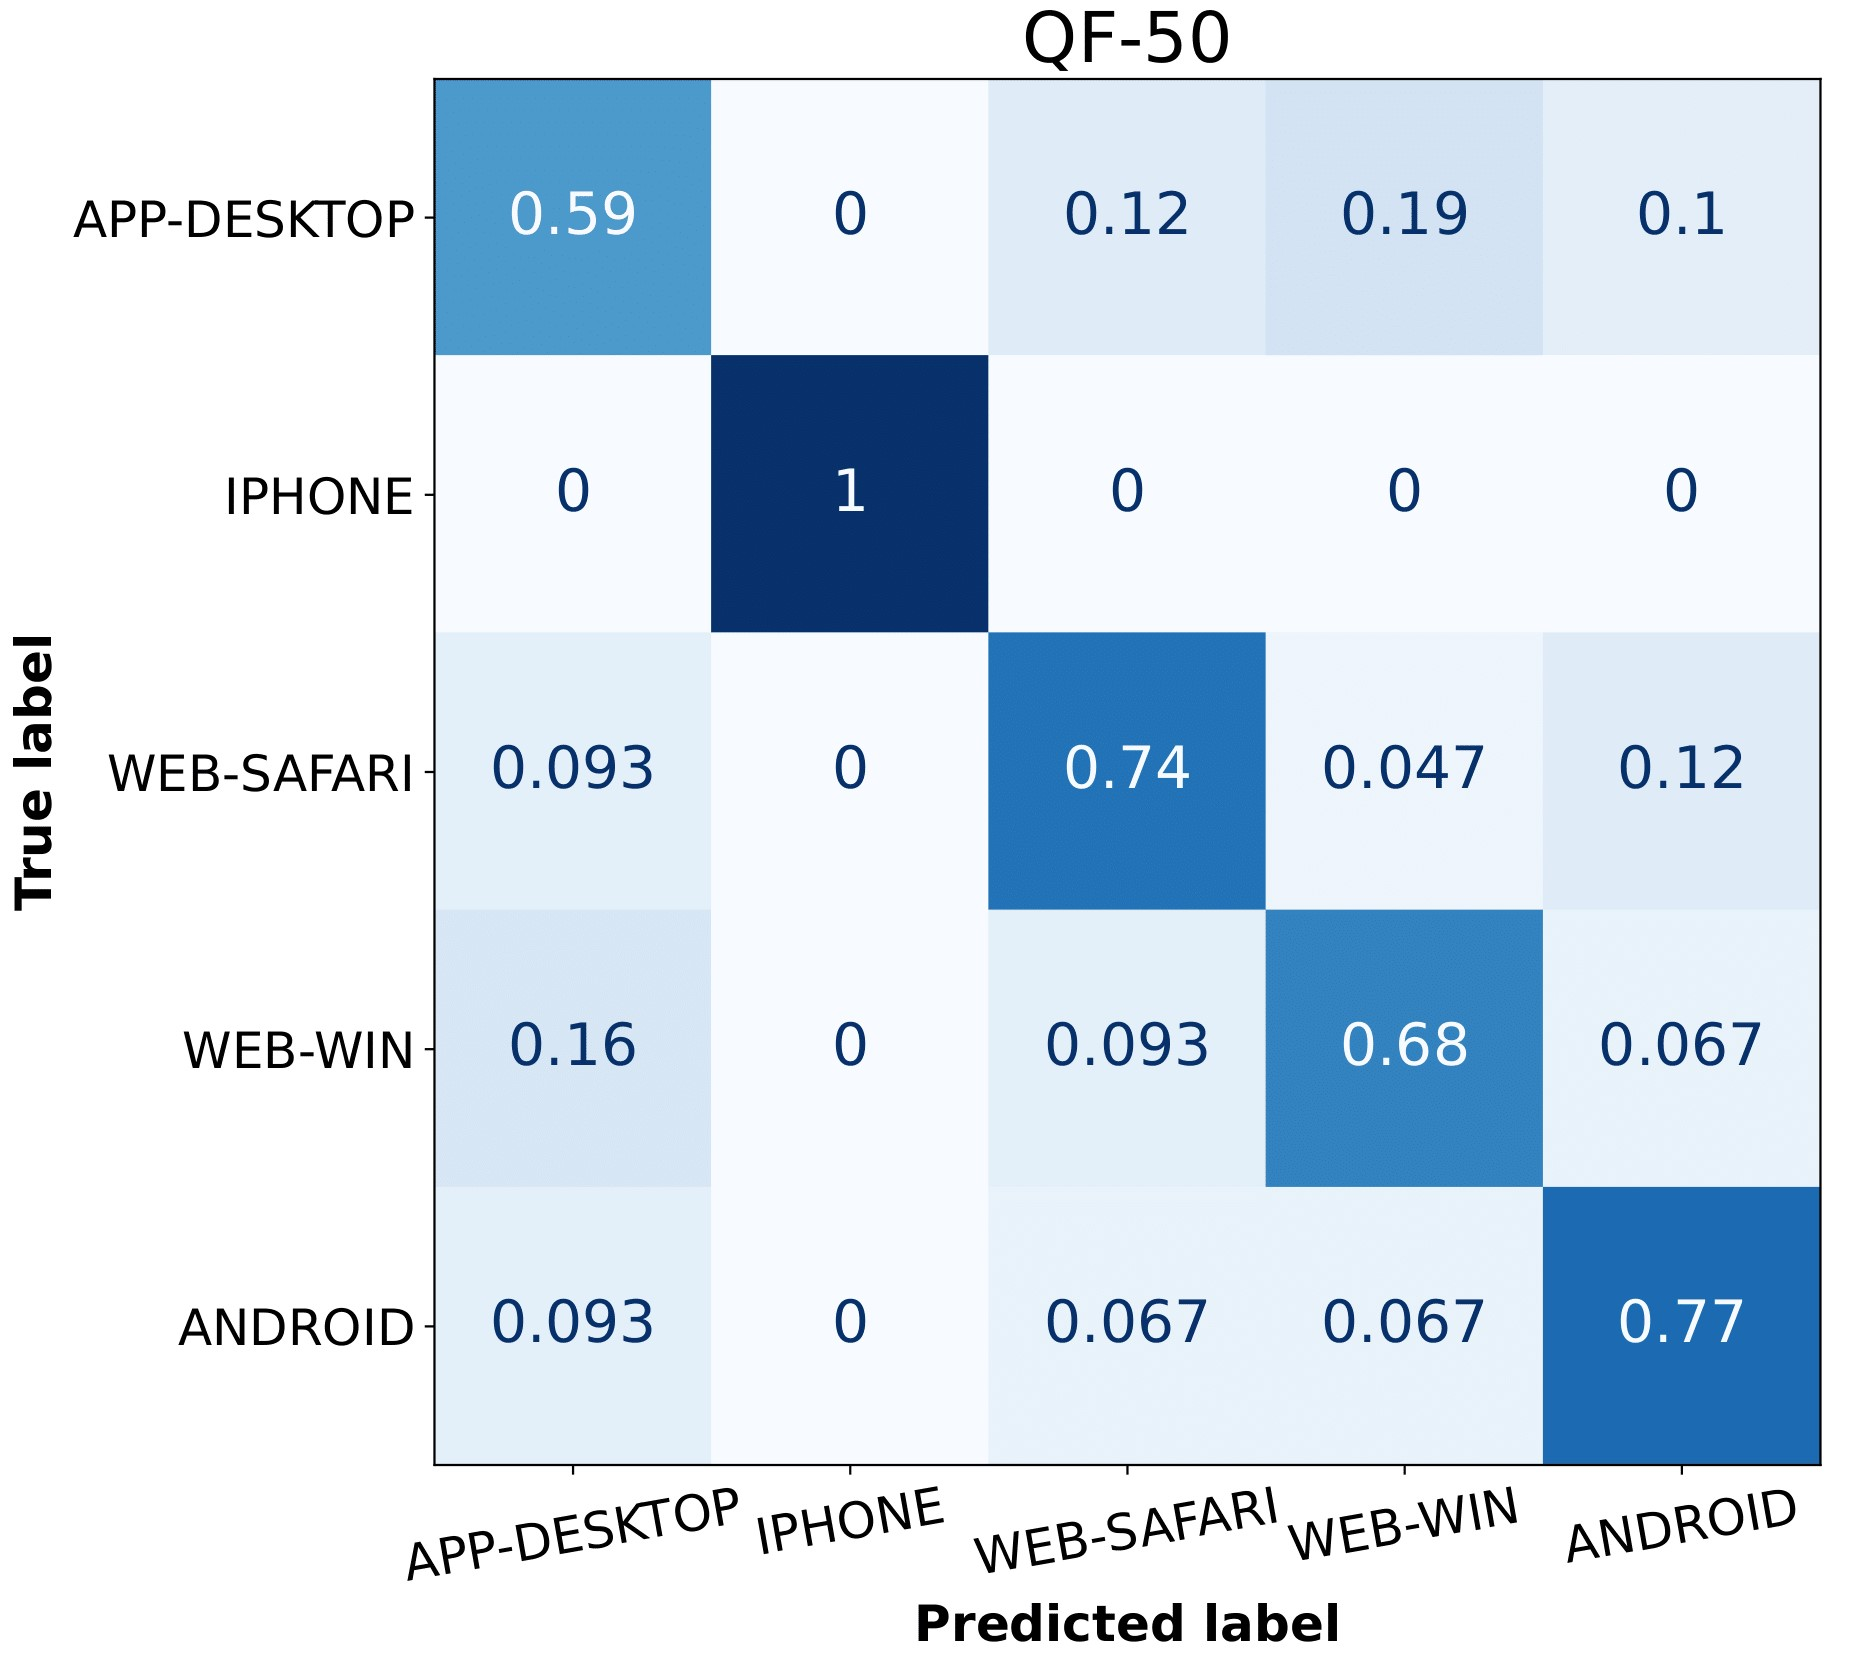
\includegraphics[width=8cm, height=8cm, keepaspectratio]{Immagini/Classificazione/confusion_matrix_RF_QF-50.jpg}\ \ \ \ \
    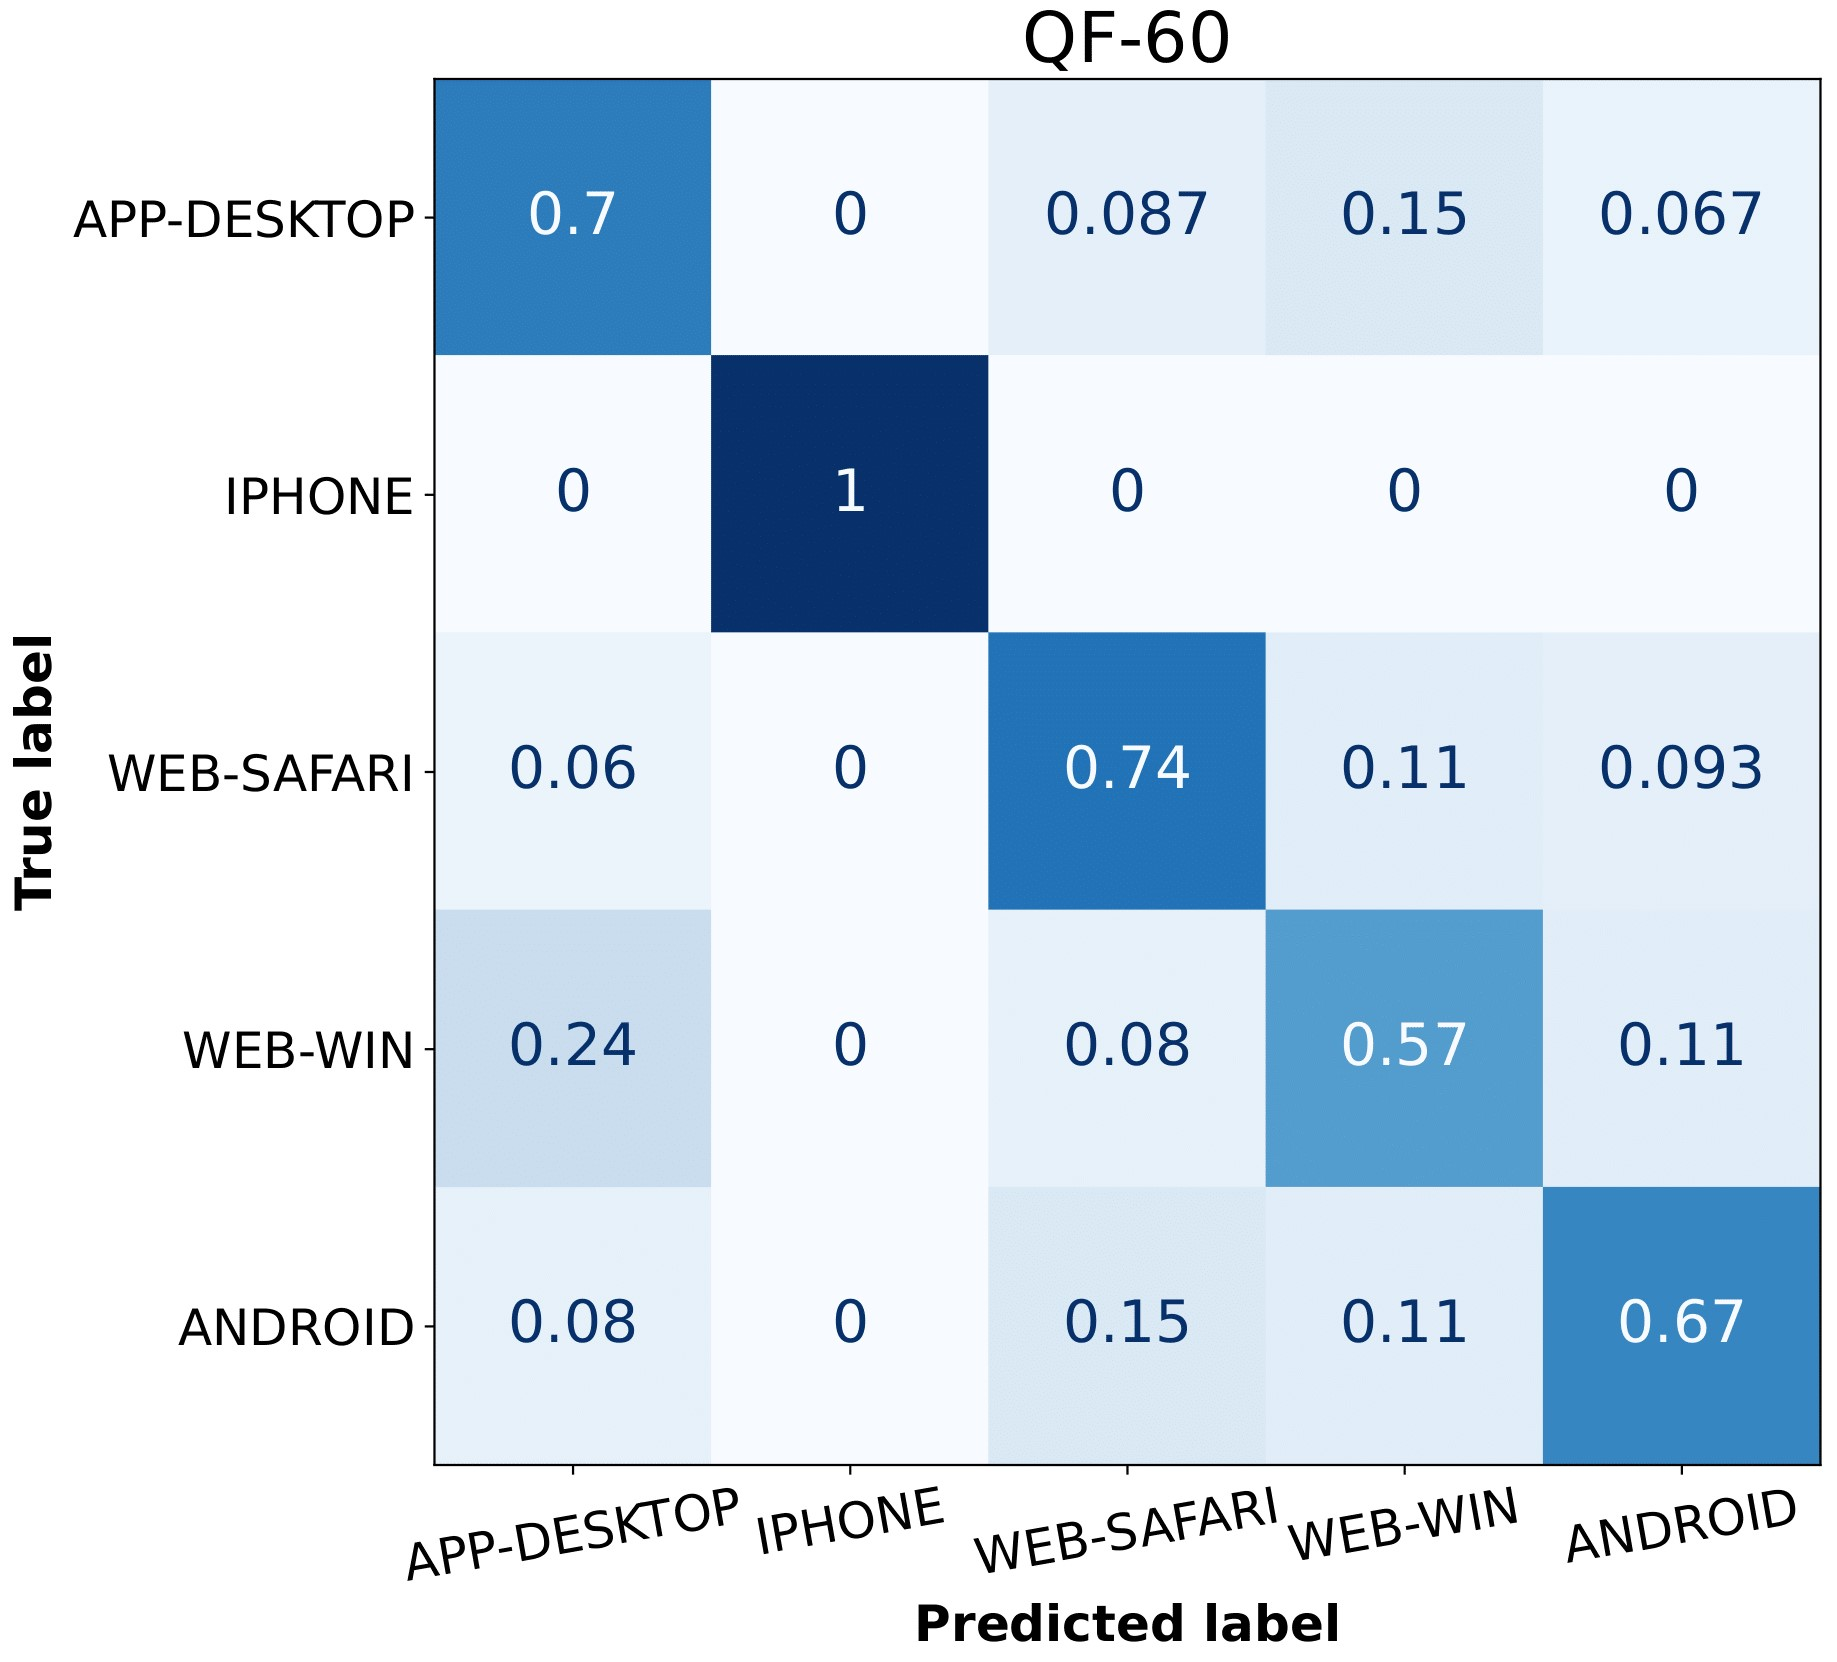
\includegraphics[width=8cm, height=8cm, keepaspectratio]{Immagini/Classificazione/confusion_matrix_RF_QF-60.jpg}\\\vspace{1em}
    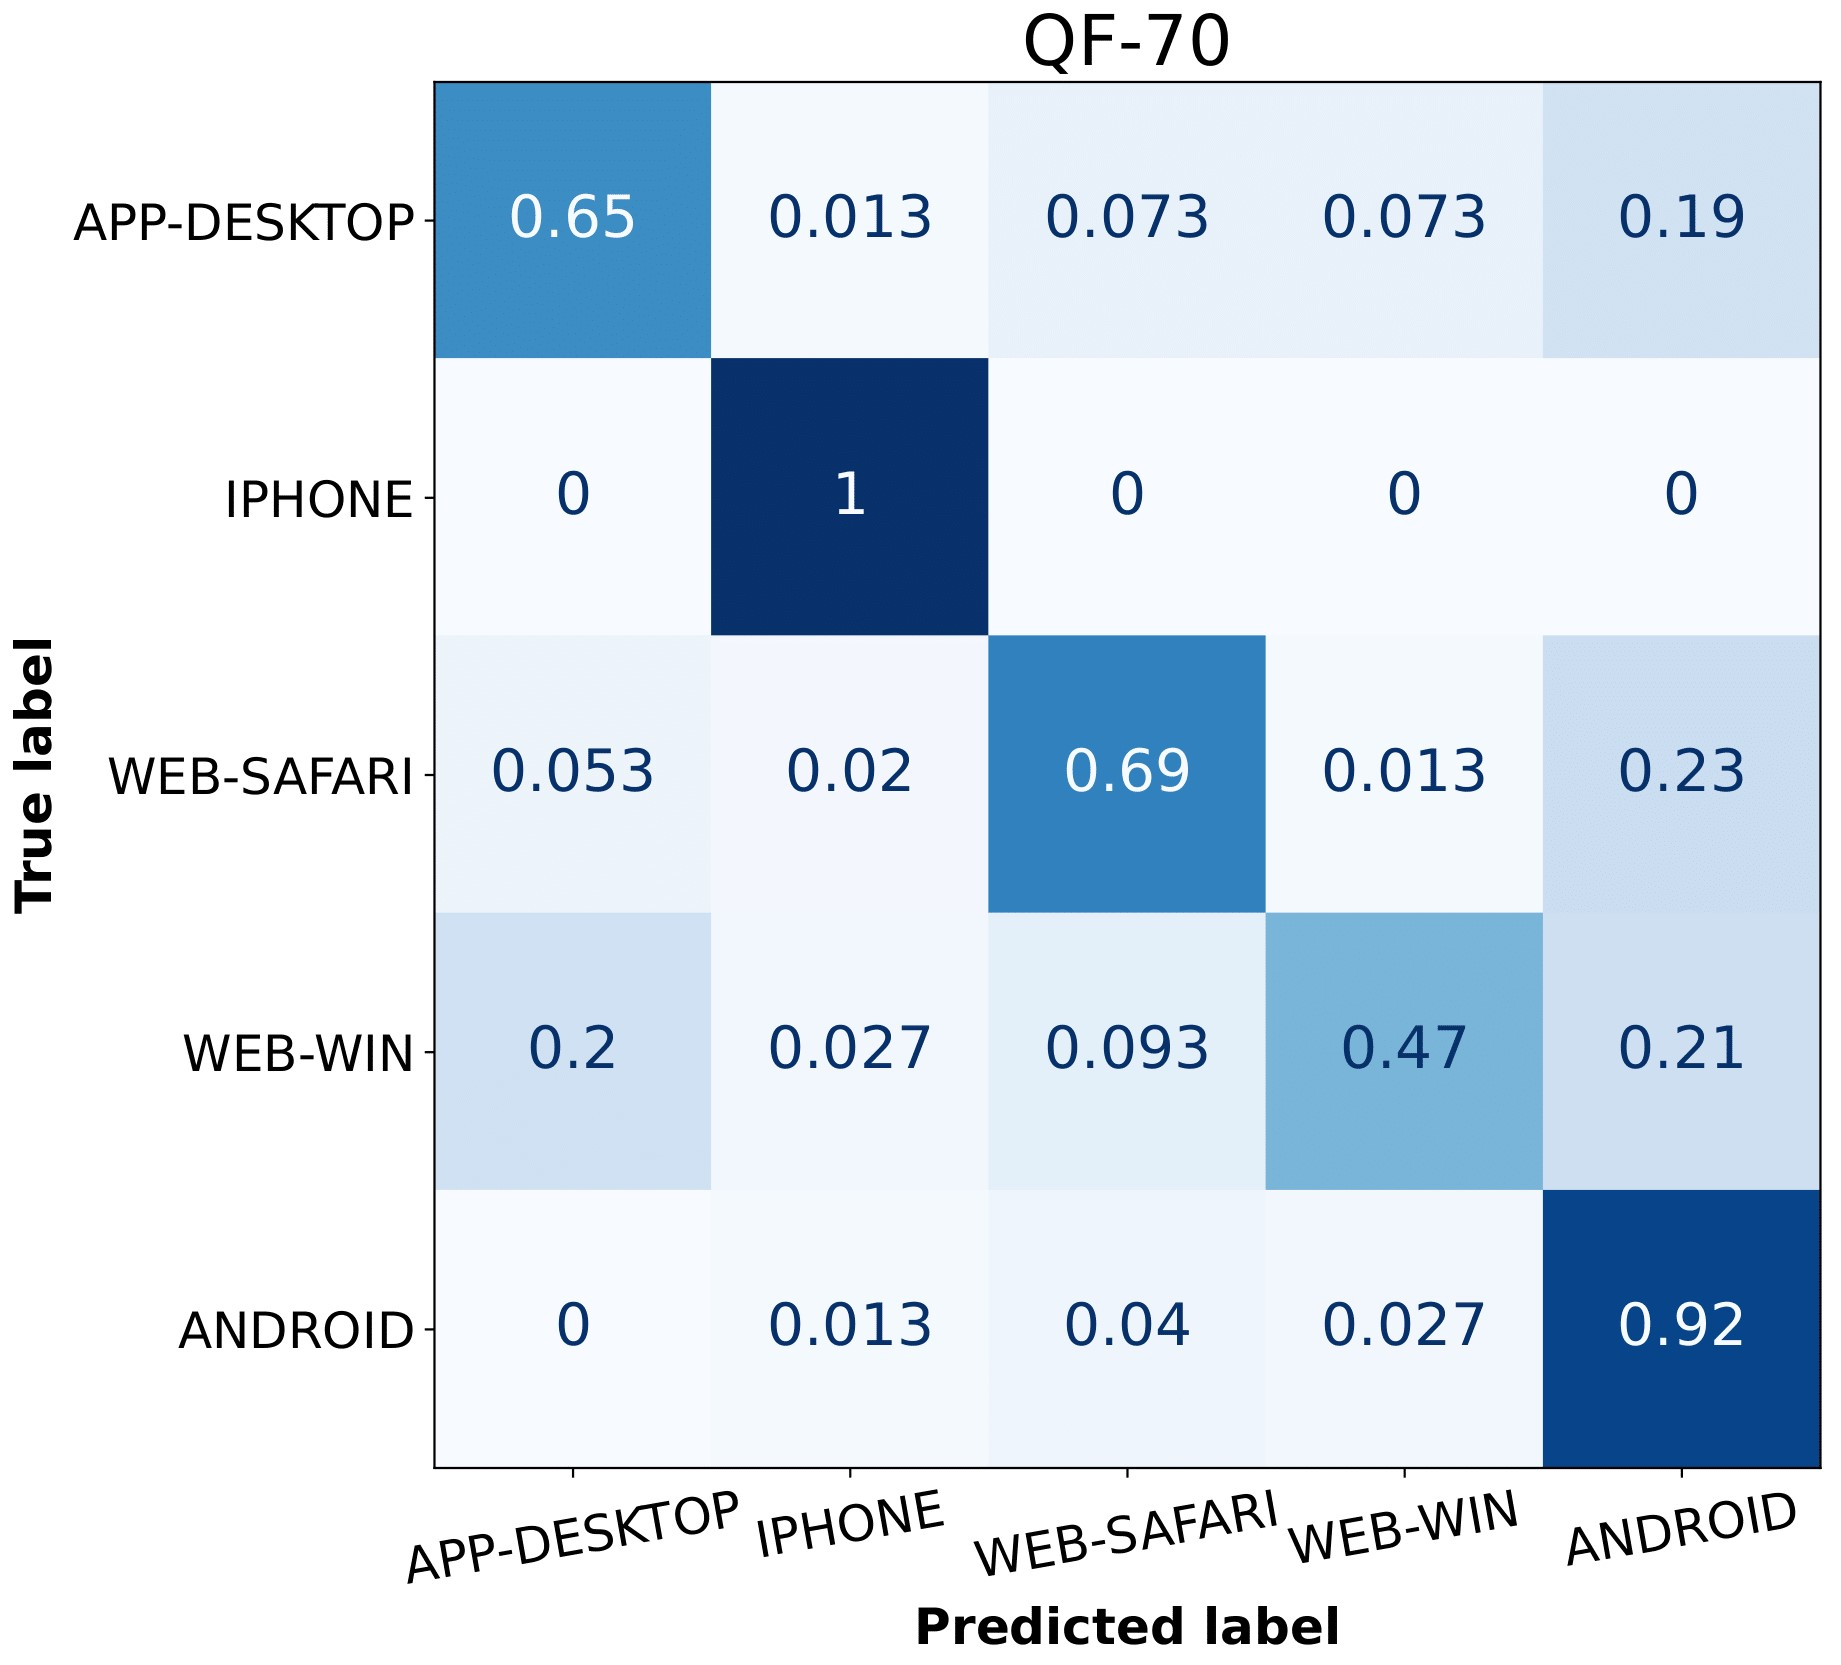
\includegraphics[width=8cm, height=8cm, keepaspectratio]{Immagini/Classificazione/confusion_matrix_RF_QF-70.jpg}\ \ \ \ \
    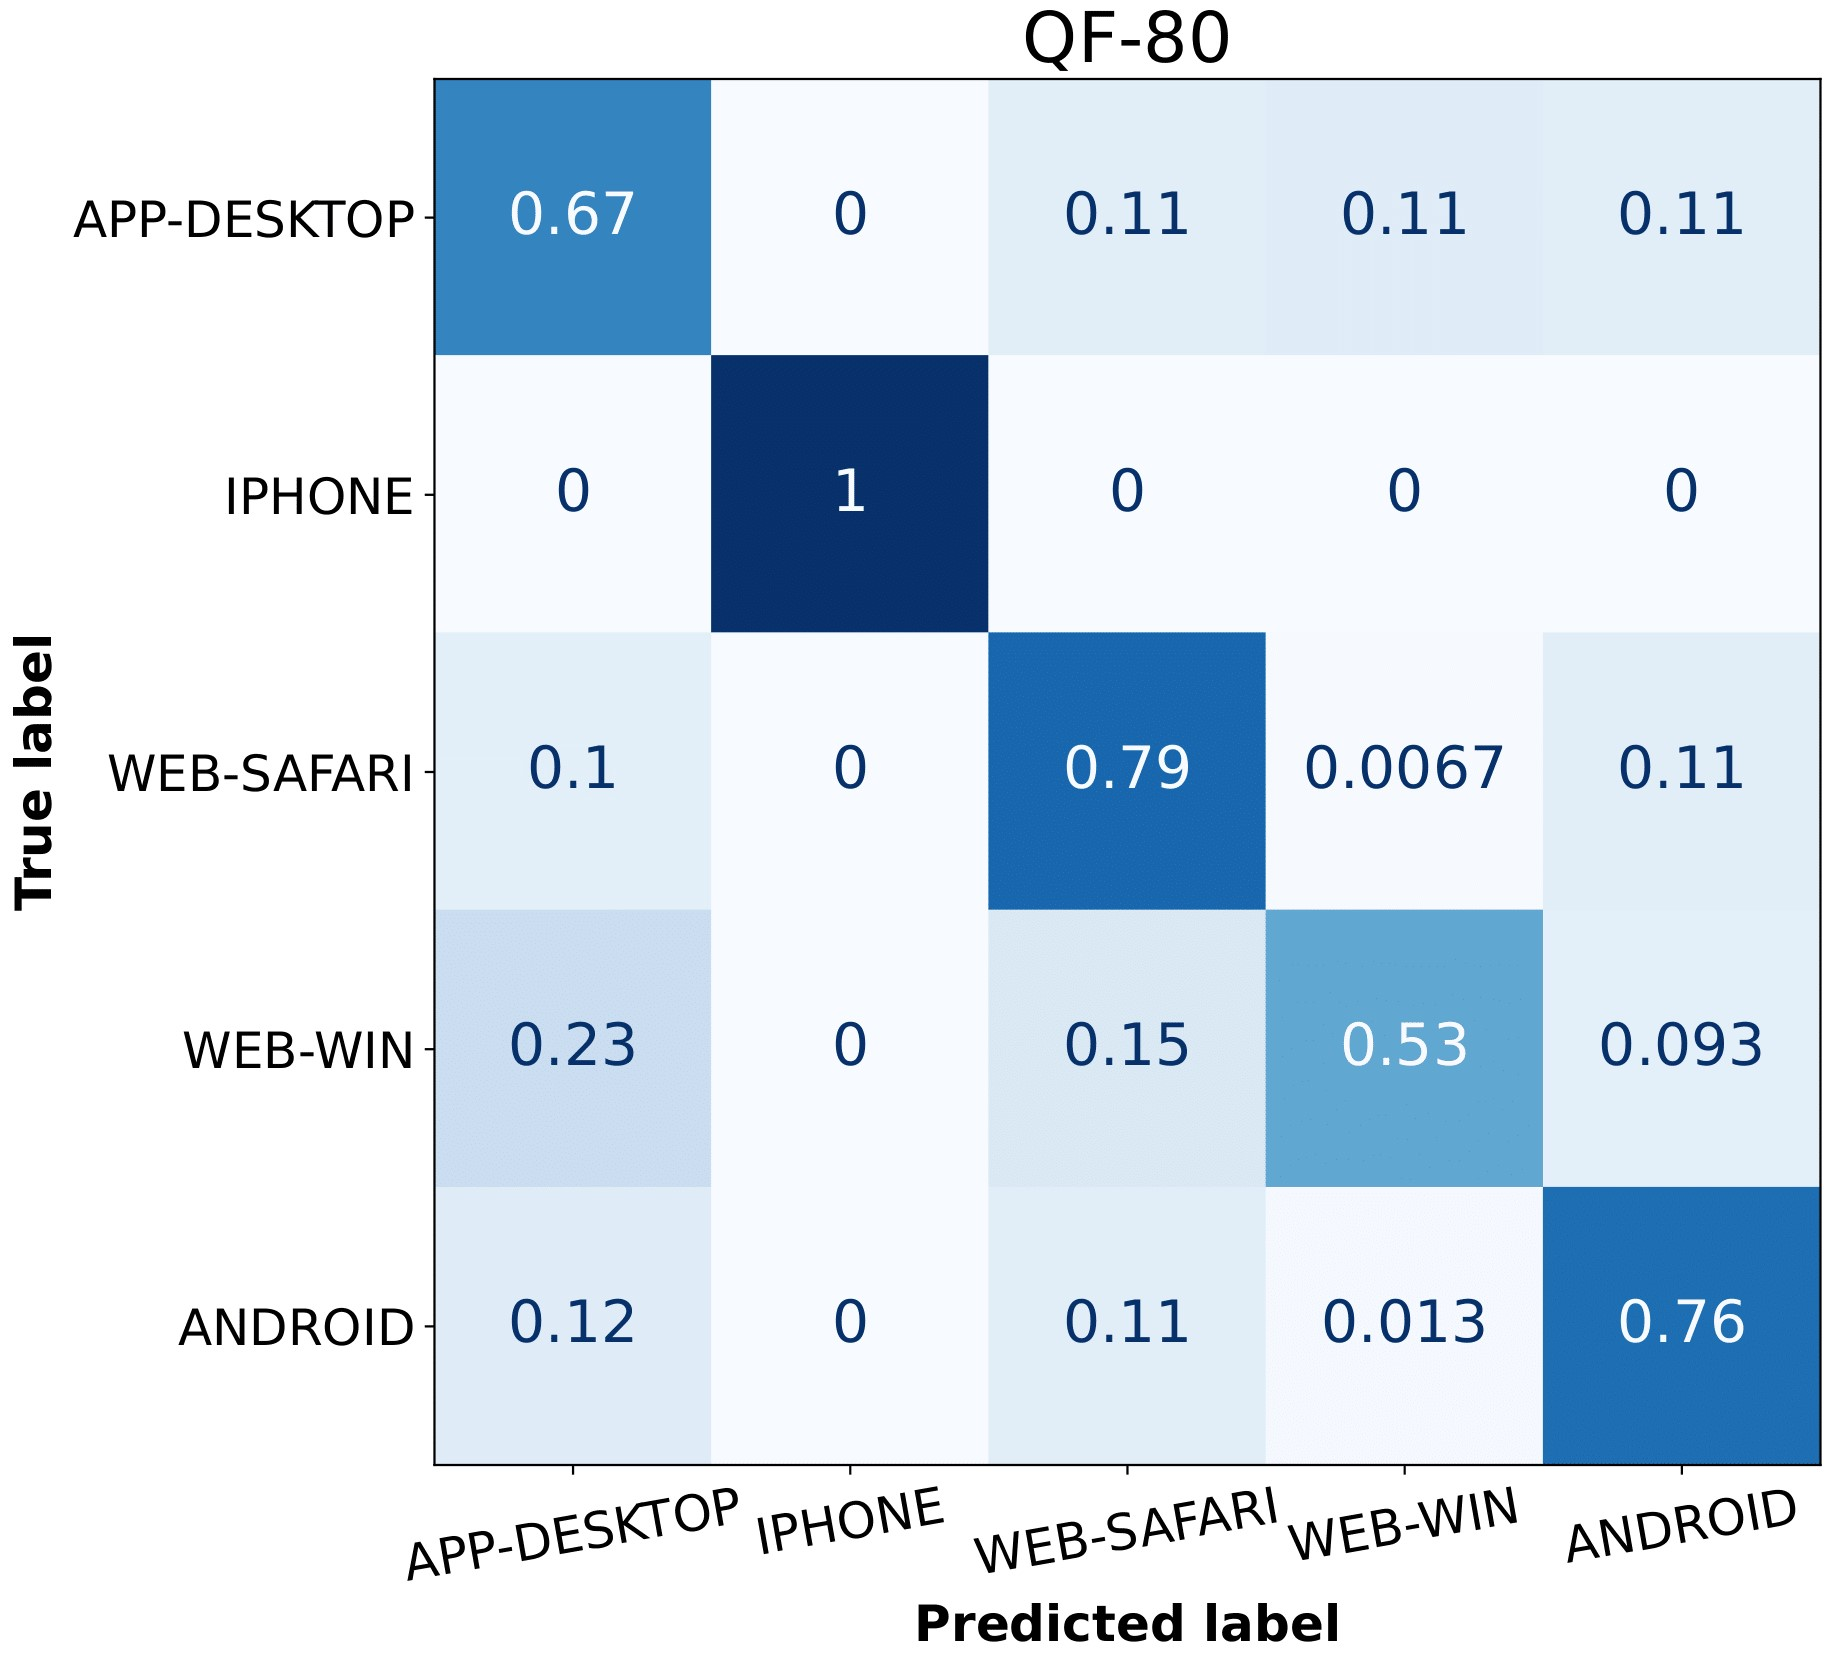
\includegraphics[width=8cm, height=8cm, keepaspectratio]{Immagini/Classificazione/confusion_matrix_RF_QF-80.jpg}\\\vspace{1em}
    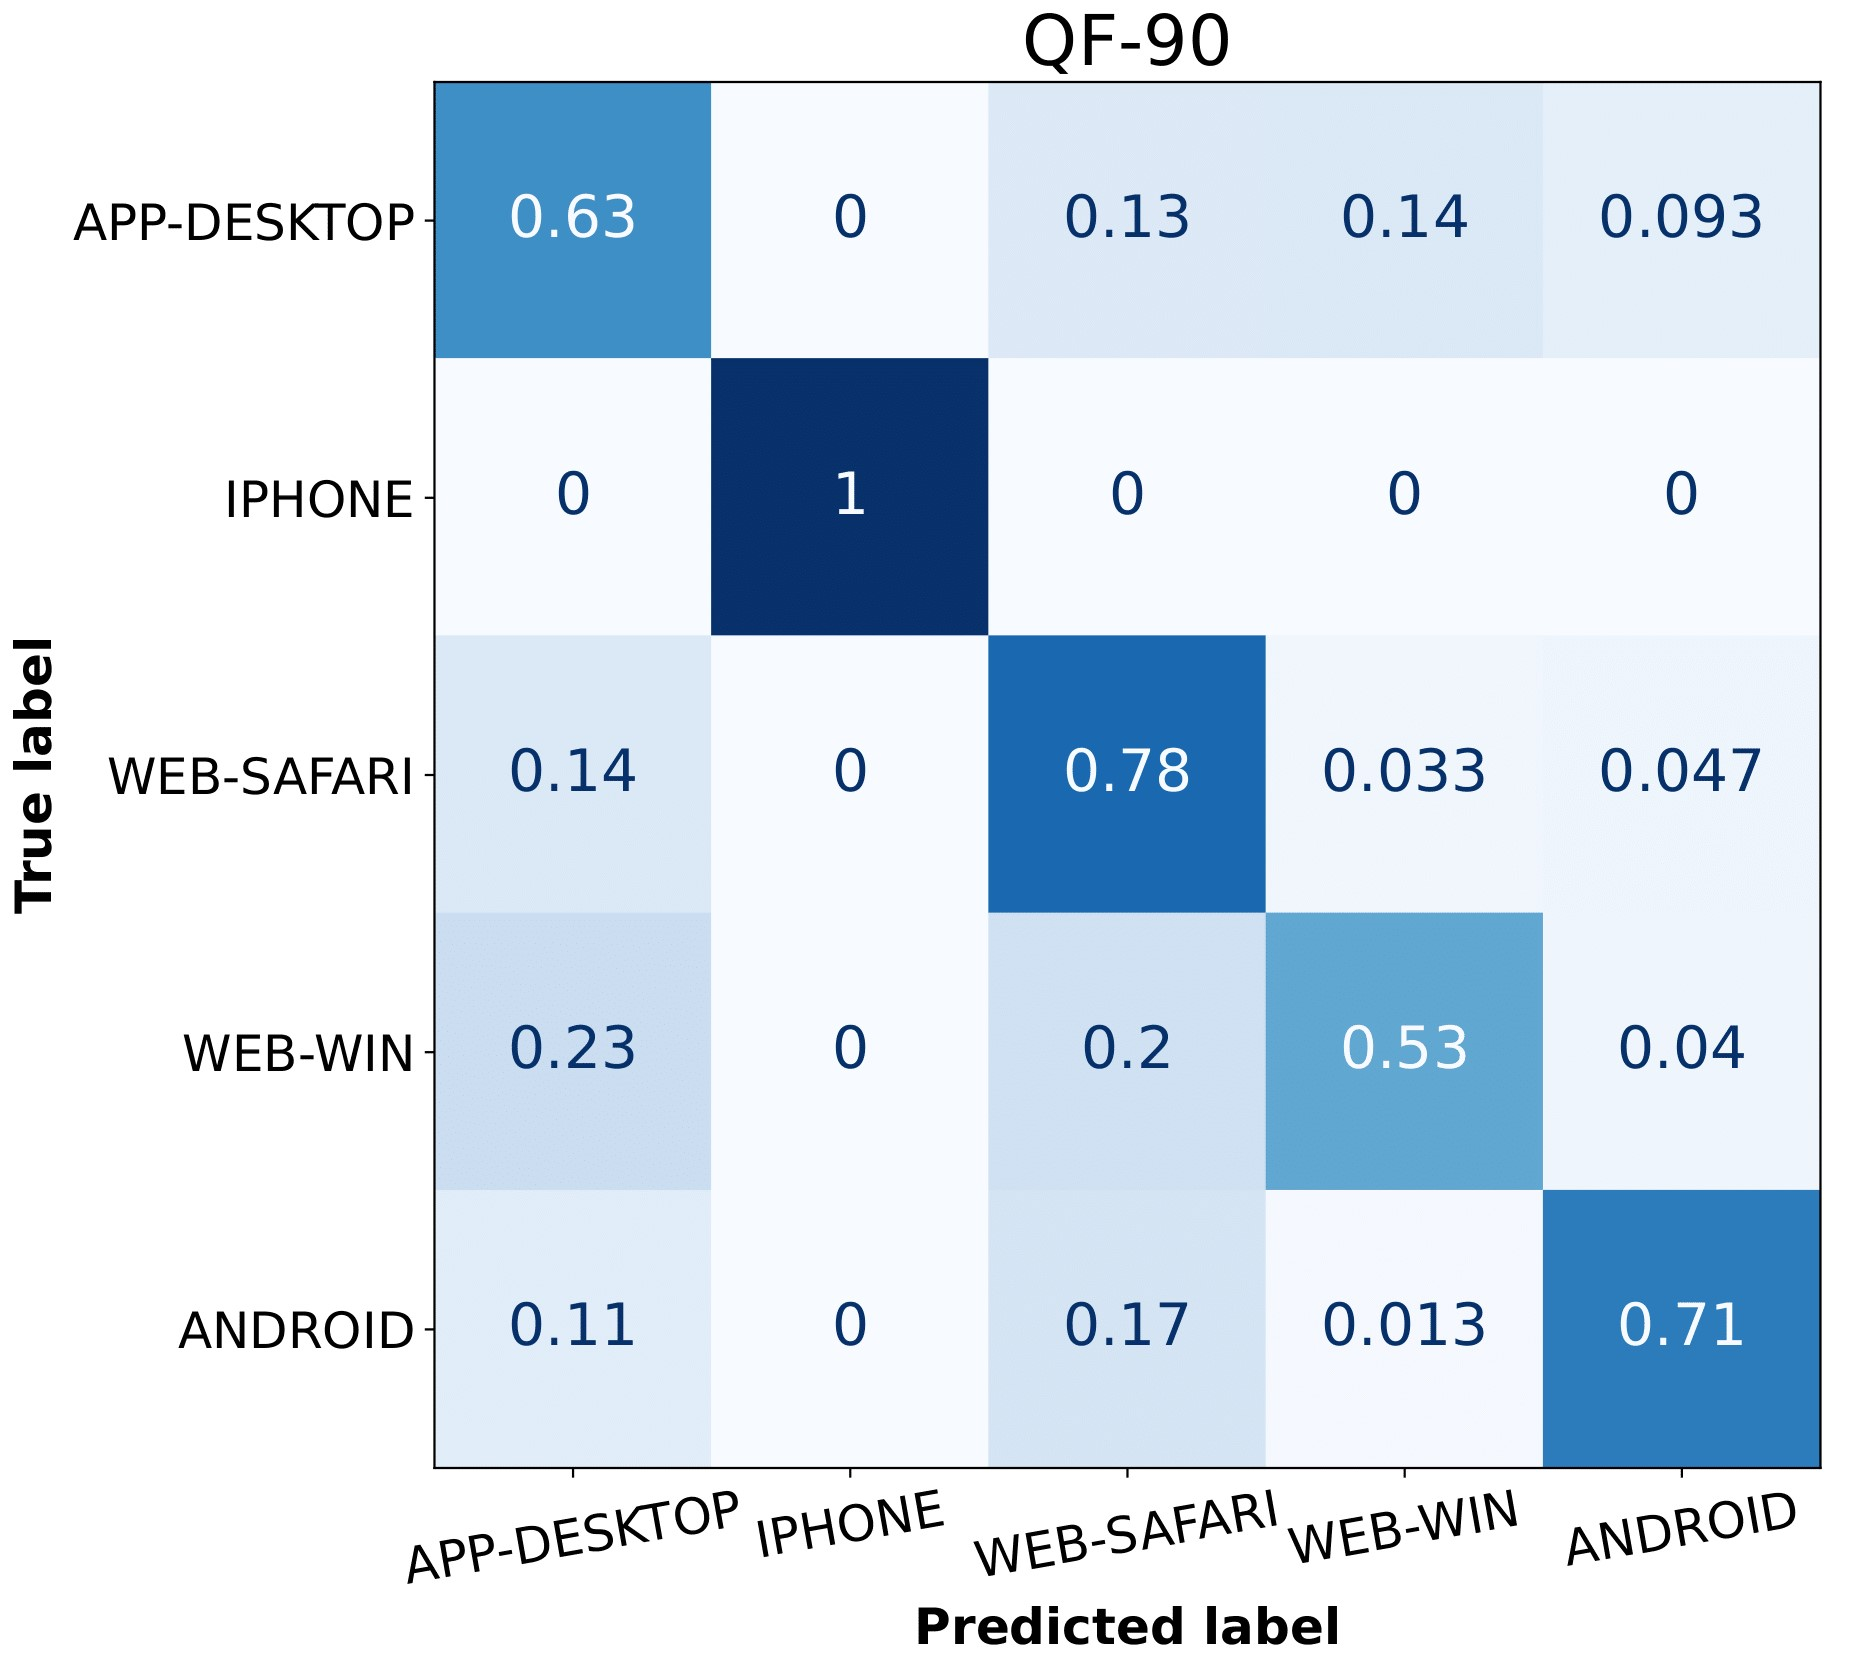
\includegraphics[width=8cm, height=8cm, keepaspectratio]{Immagini/Classificazione/confusion_matrix_RF_QF-90.jpg}\ \ \ \ \
    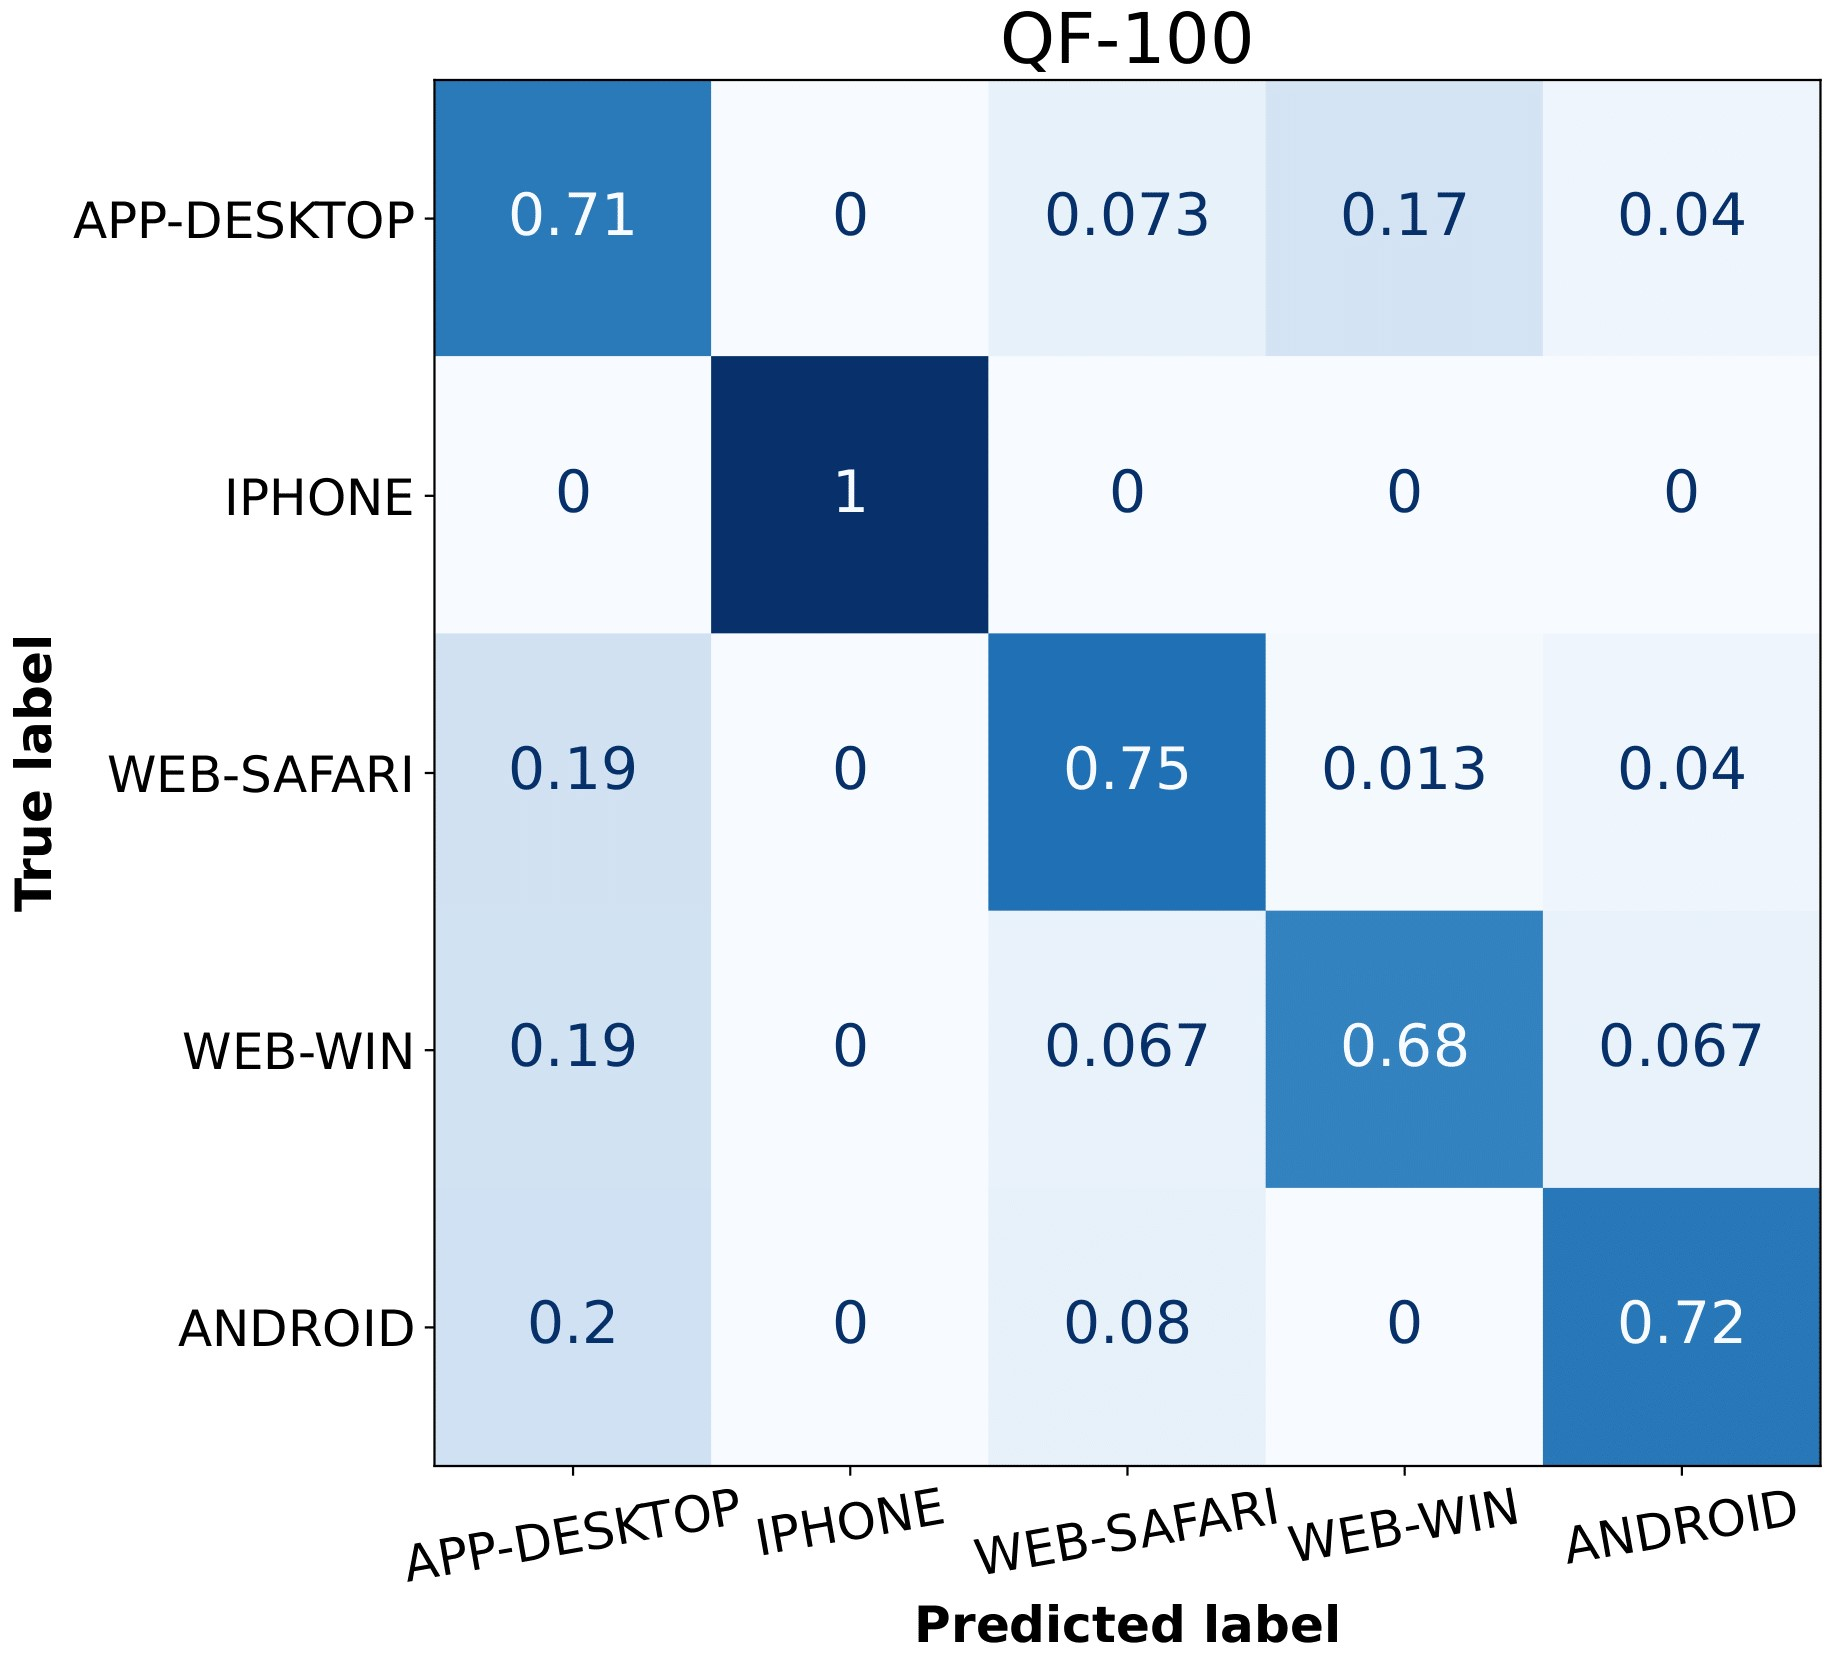
\includegraphics[width=8cm, height=8cm, keepaspectratio]{Immagini/Classificazione/confusion_matrix_RF_QF-100.jpg}
    \captionof{figure}{\textit{Confusion matrix} per \textit{random forest} divise per \textit{quality factor}.}
    \label{fig:class_QF_RF}
\endgroup

\vspace{3em}

\begingroup
    \centering
    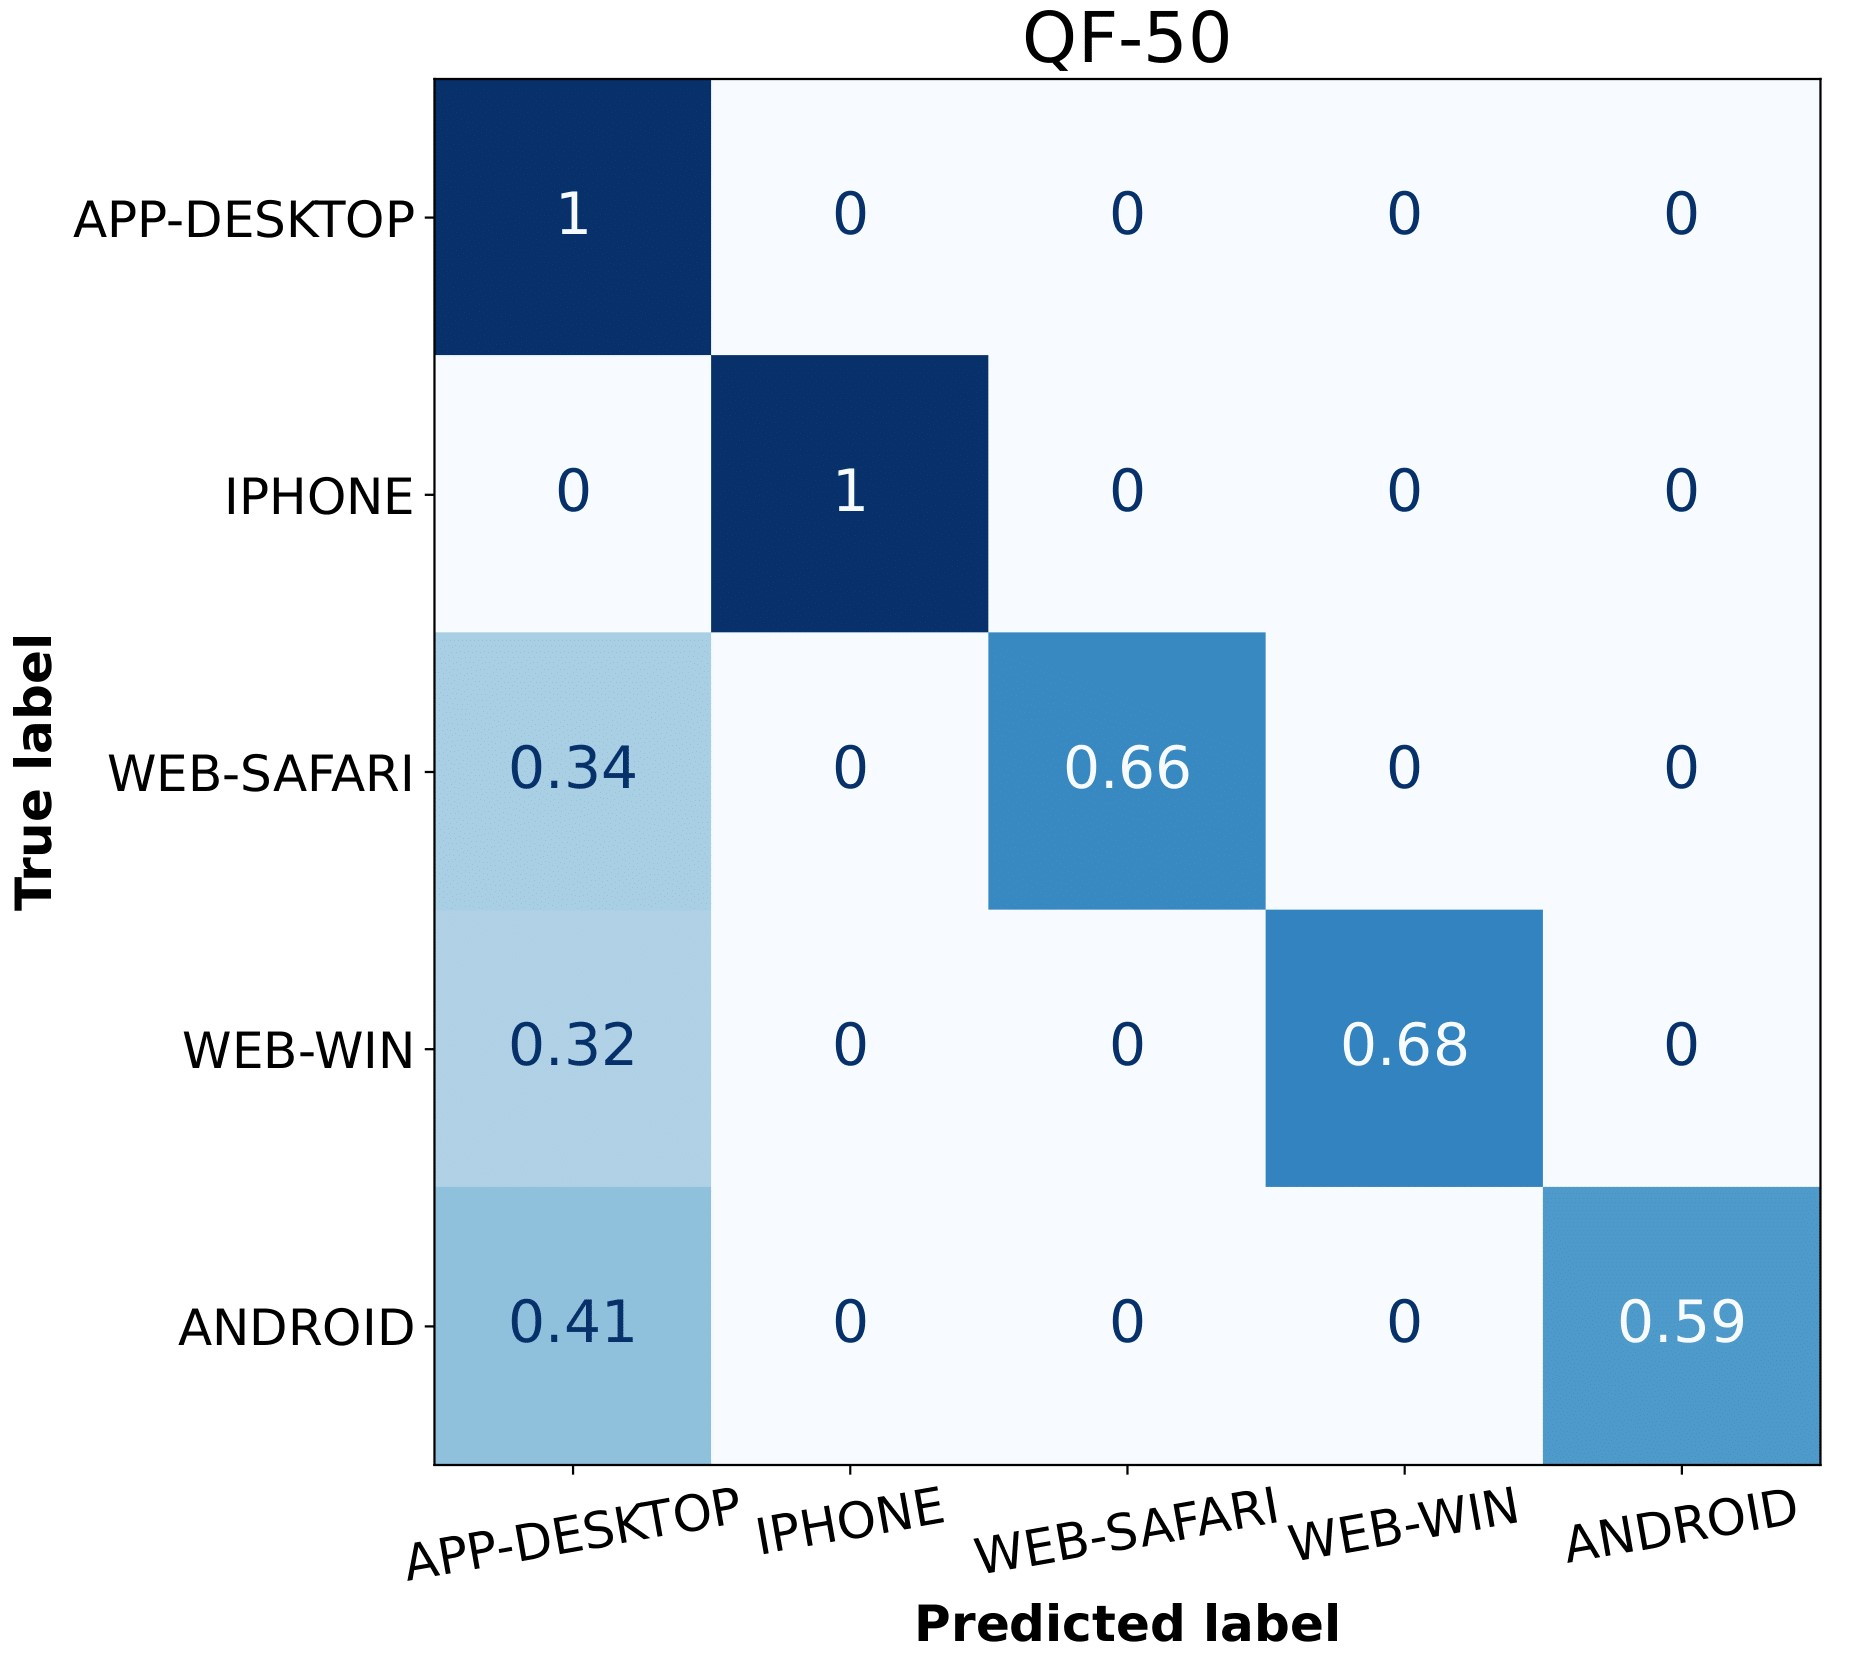
\includegraphics[width=8cm, height=8cm, keepaspectratio]{Immagini/Classificazione/confusion_matrix_SVM_QF-50.jpg}\ \ \ \ \
    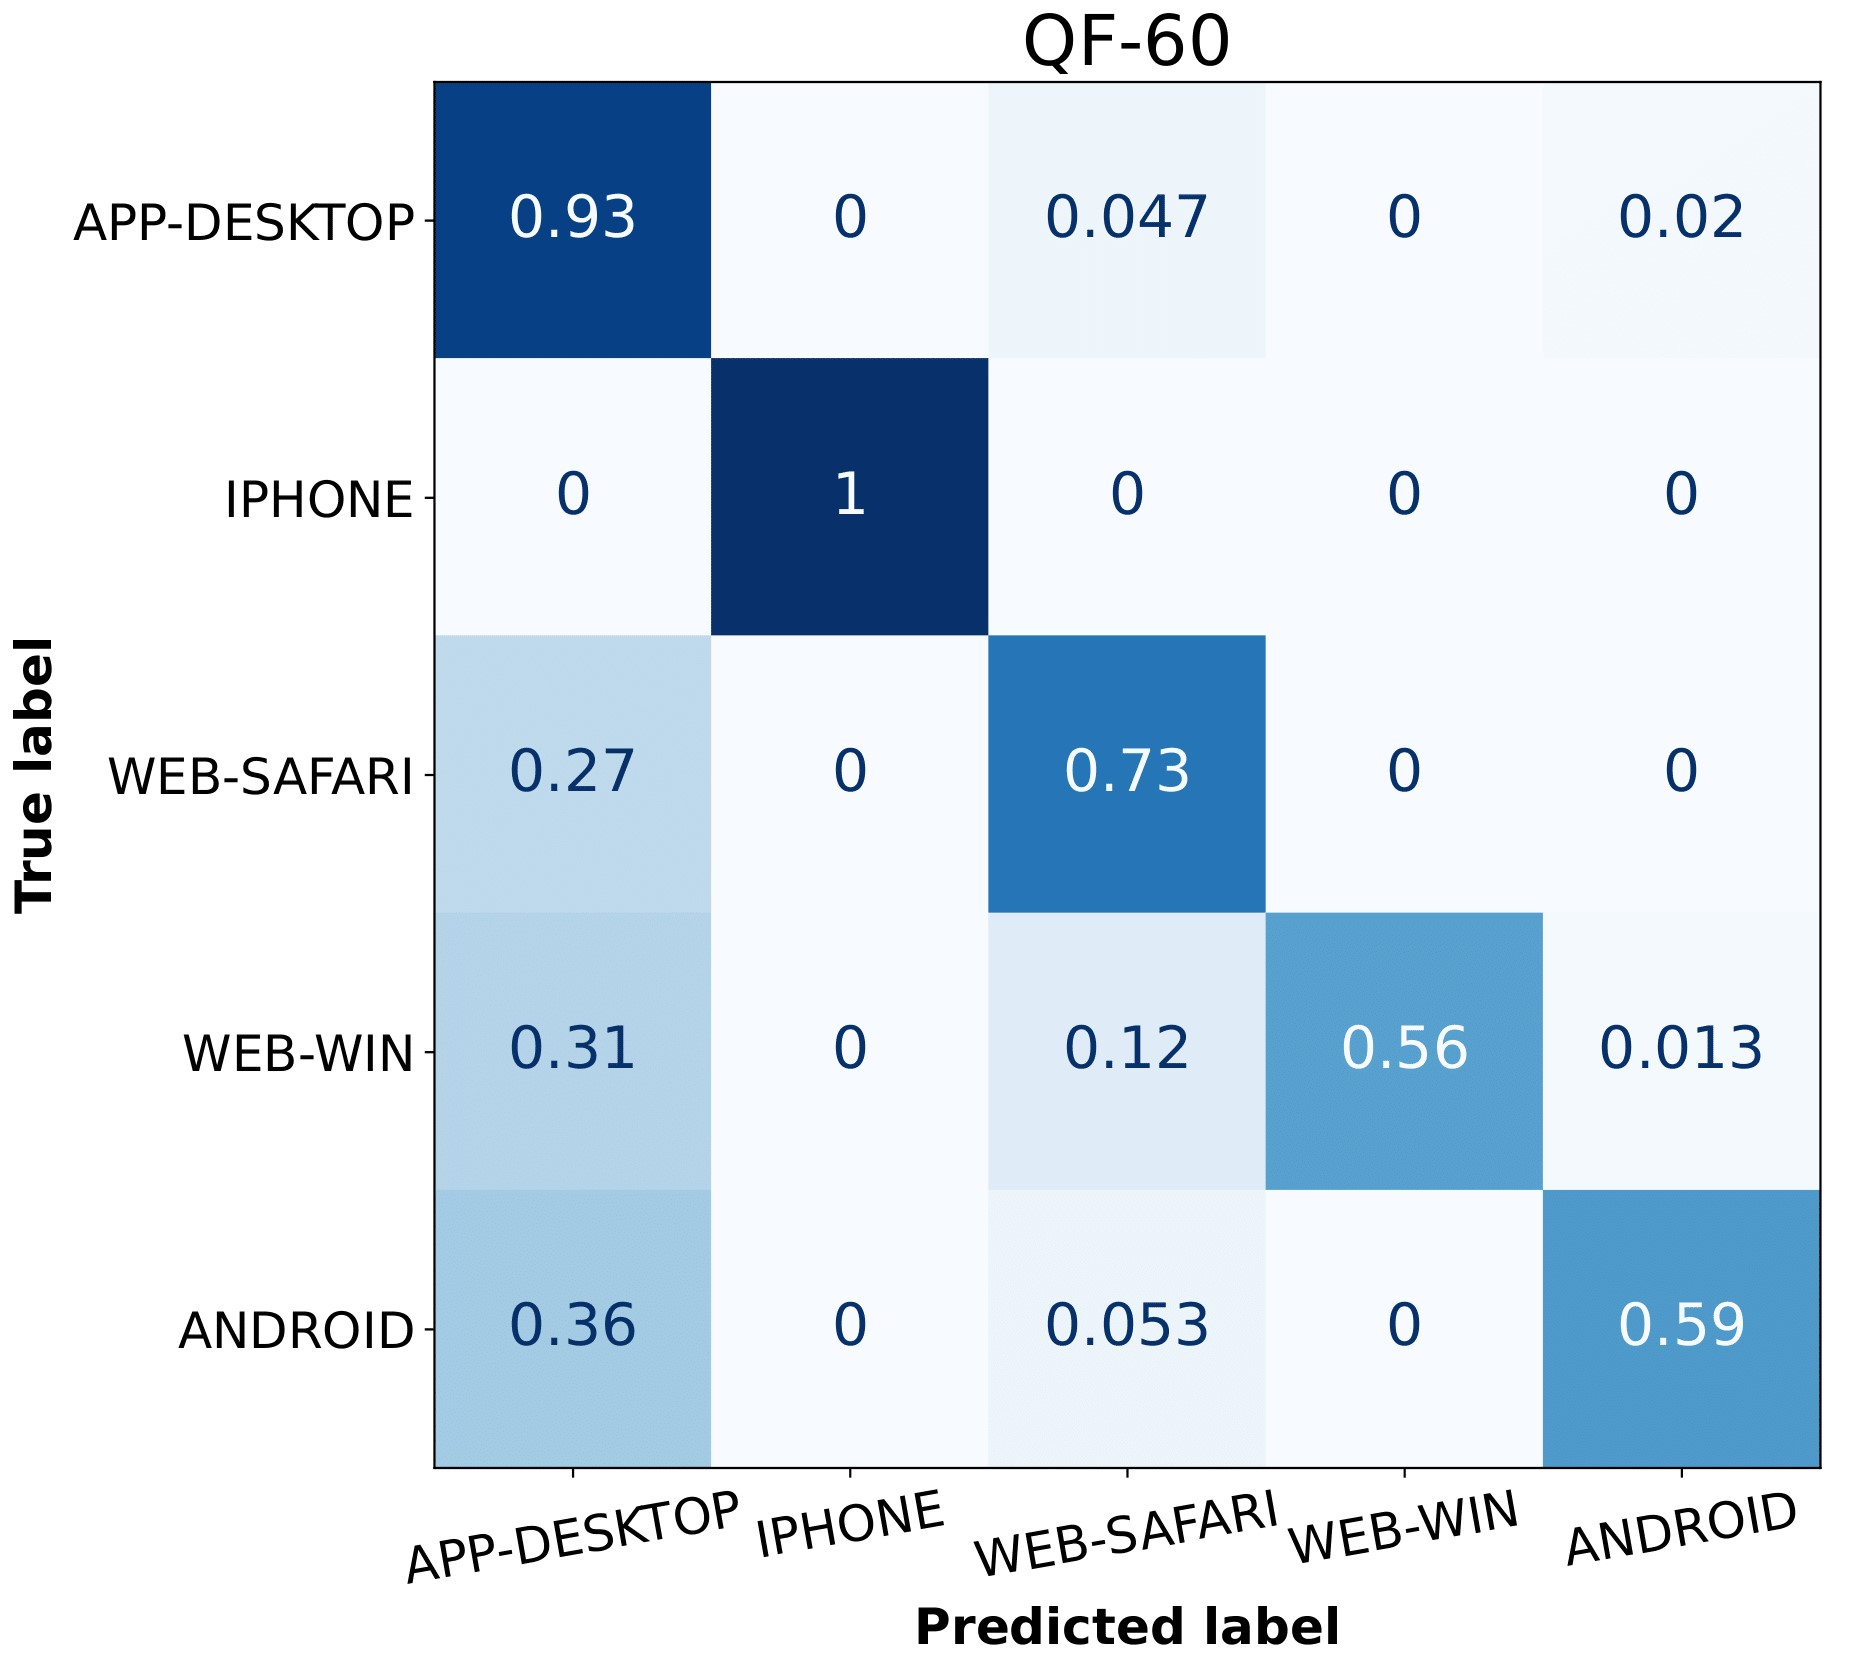
\includegraphics[width=8cm, height=8cm, keepaspectratio]{Immagini/Classificazione/confusion_matrix_SVM_QF-60.jpg}\\\vspace{1em}
    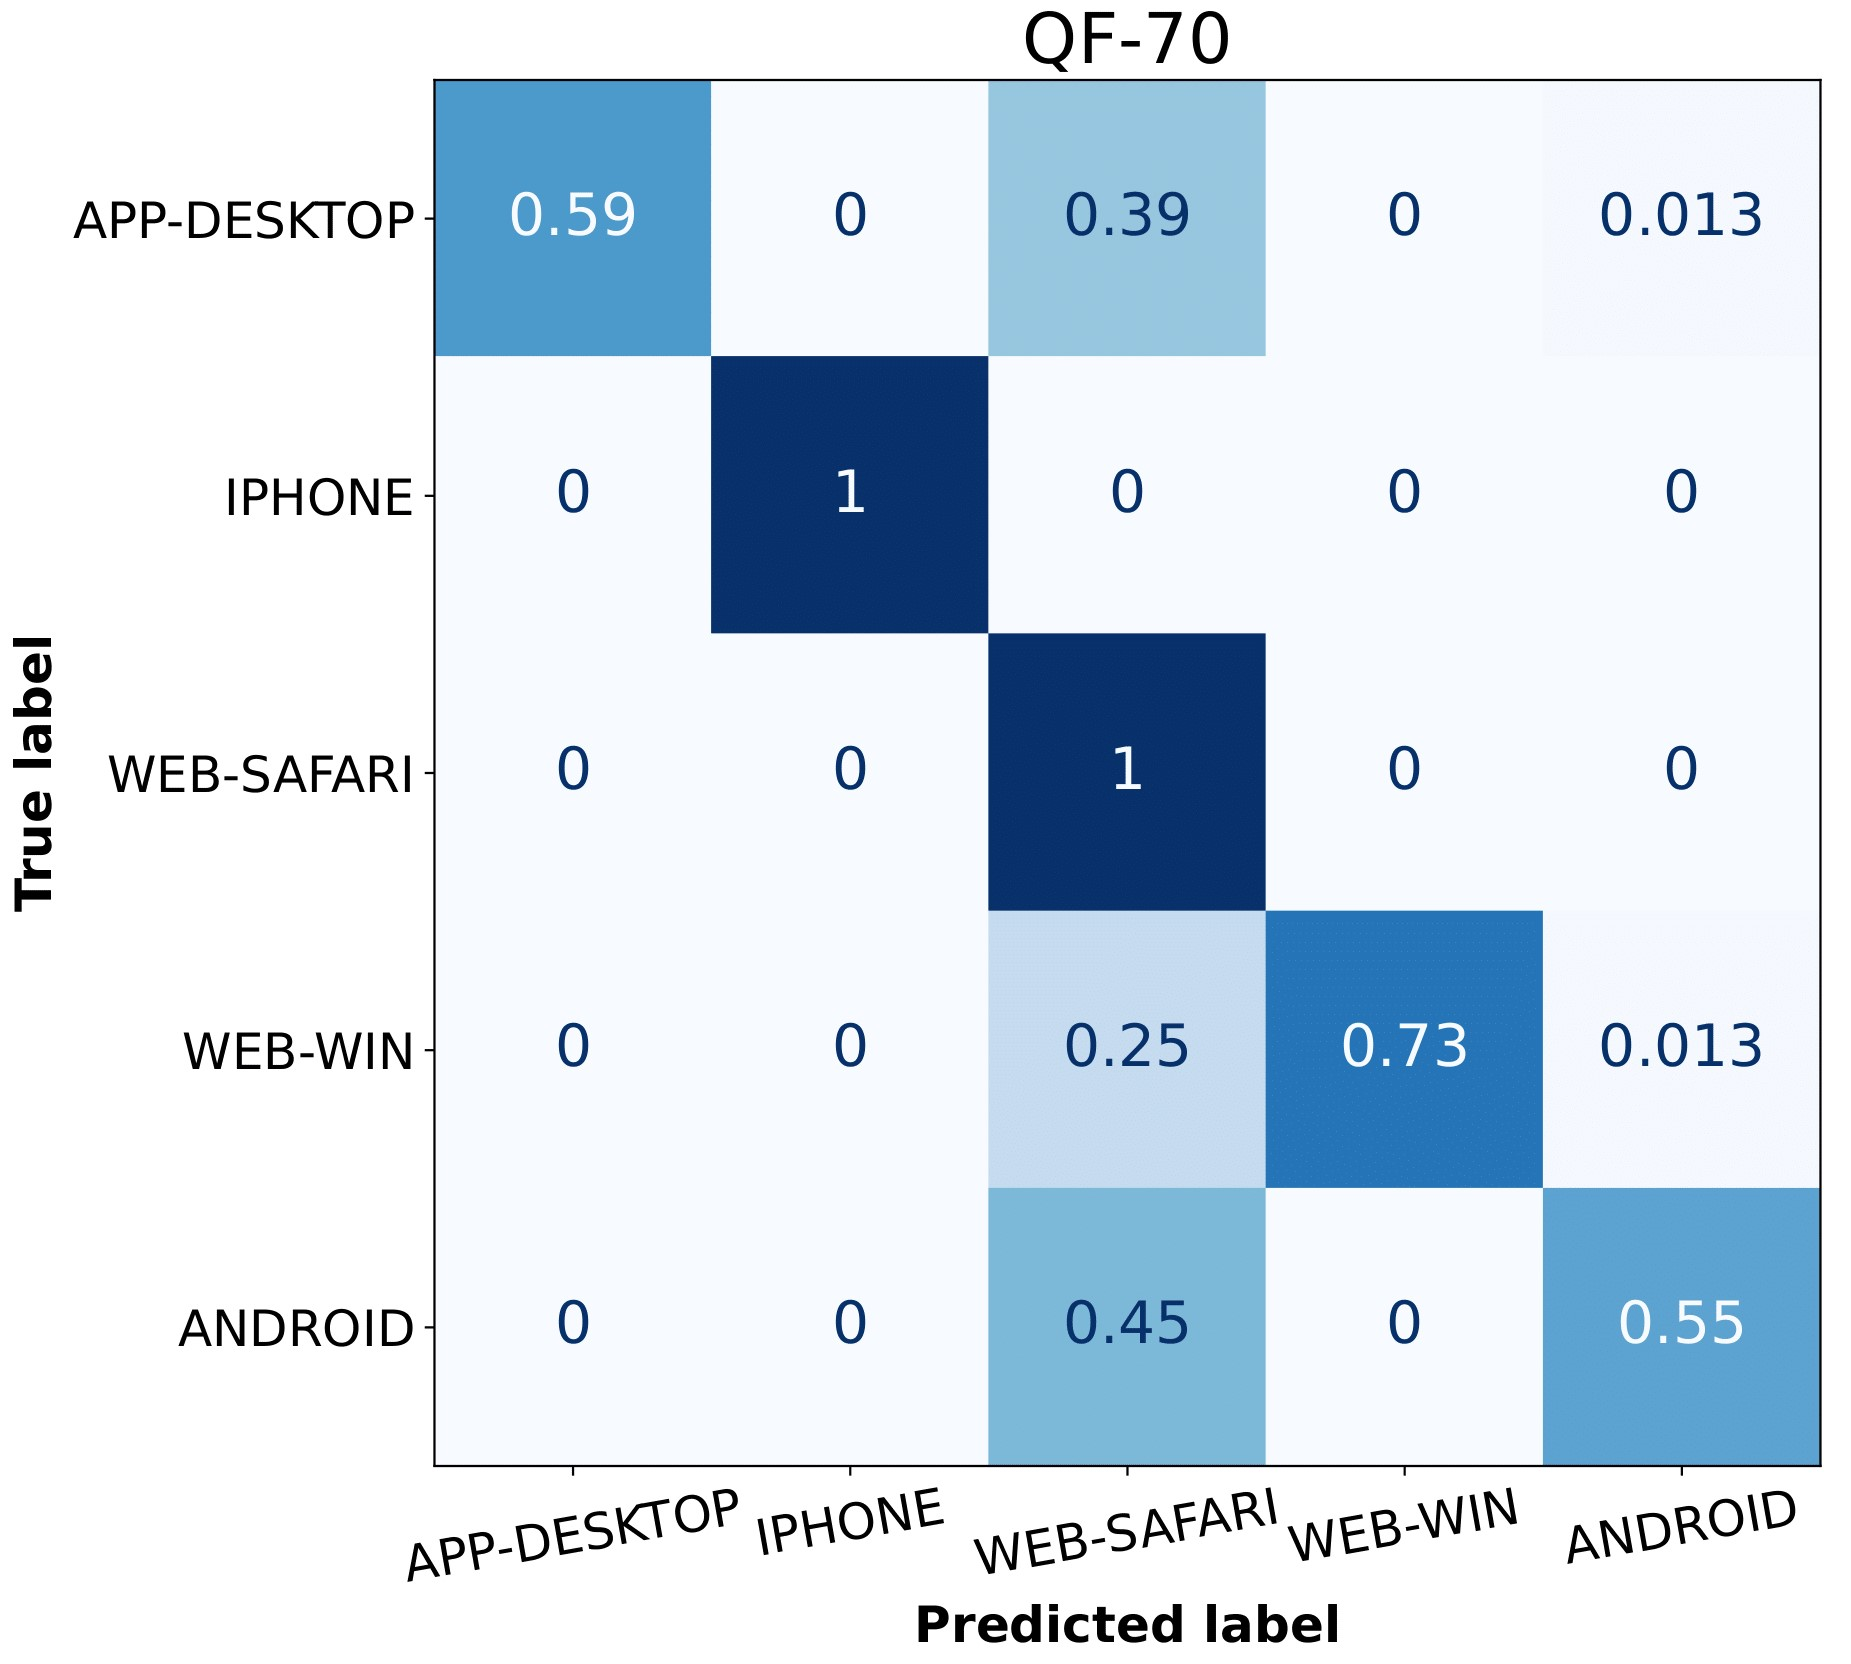
\includegraphics[width=8cm, height=8cm, keepaspectratio]{Immagini/Classificazione/confusion_matrix_SVM_QF-70.jpg}\ \ \ \ \
    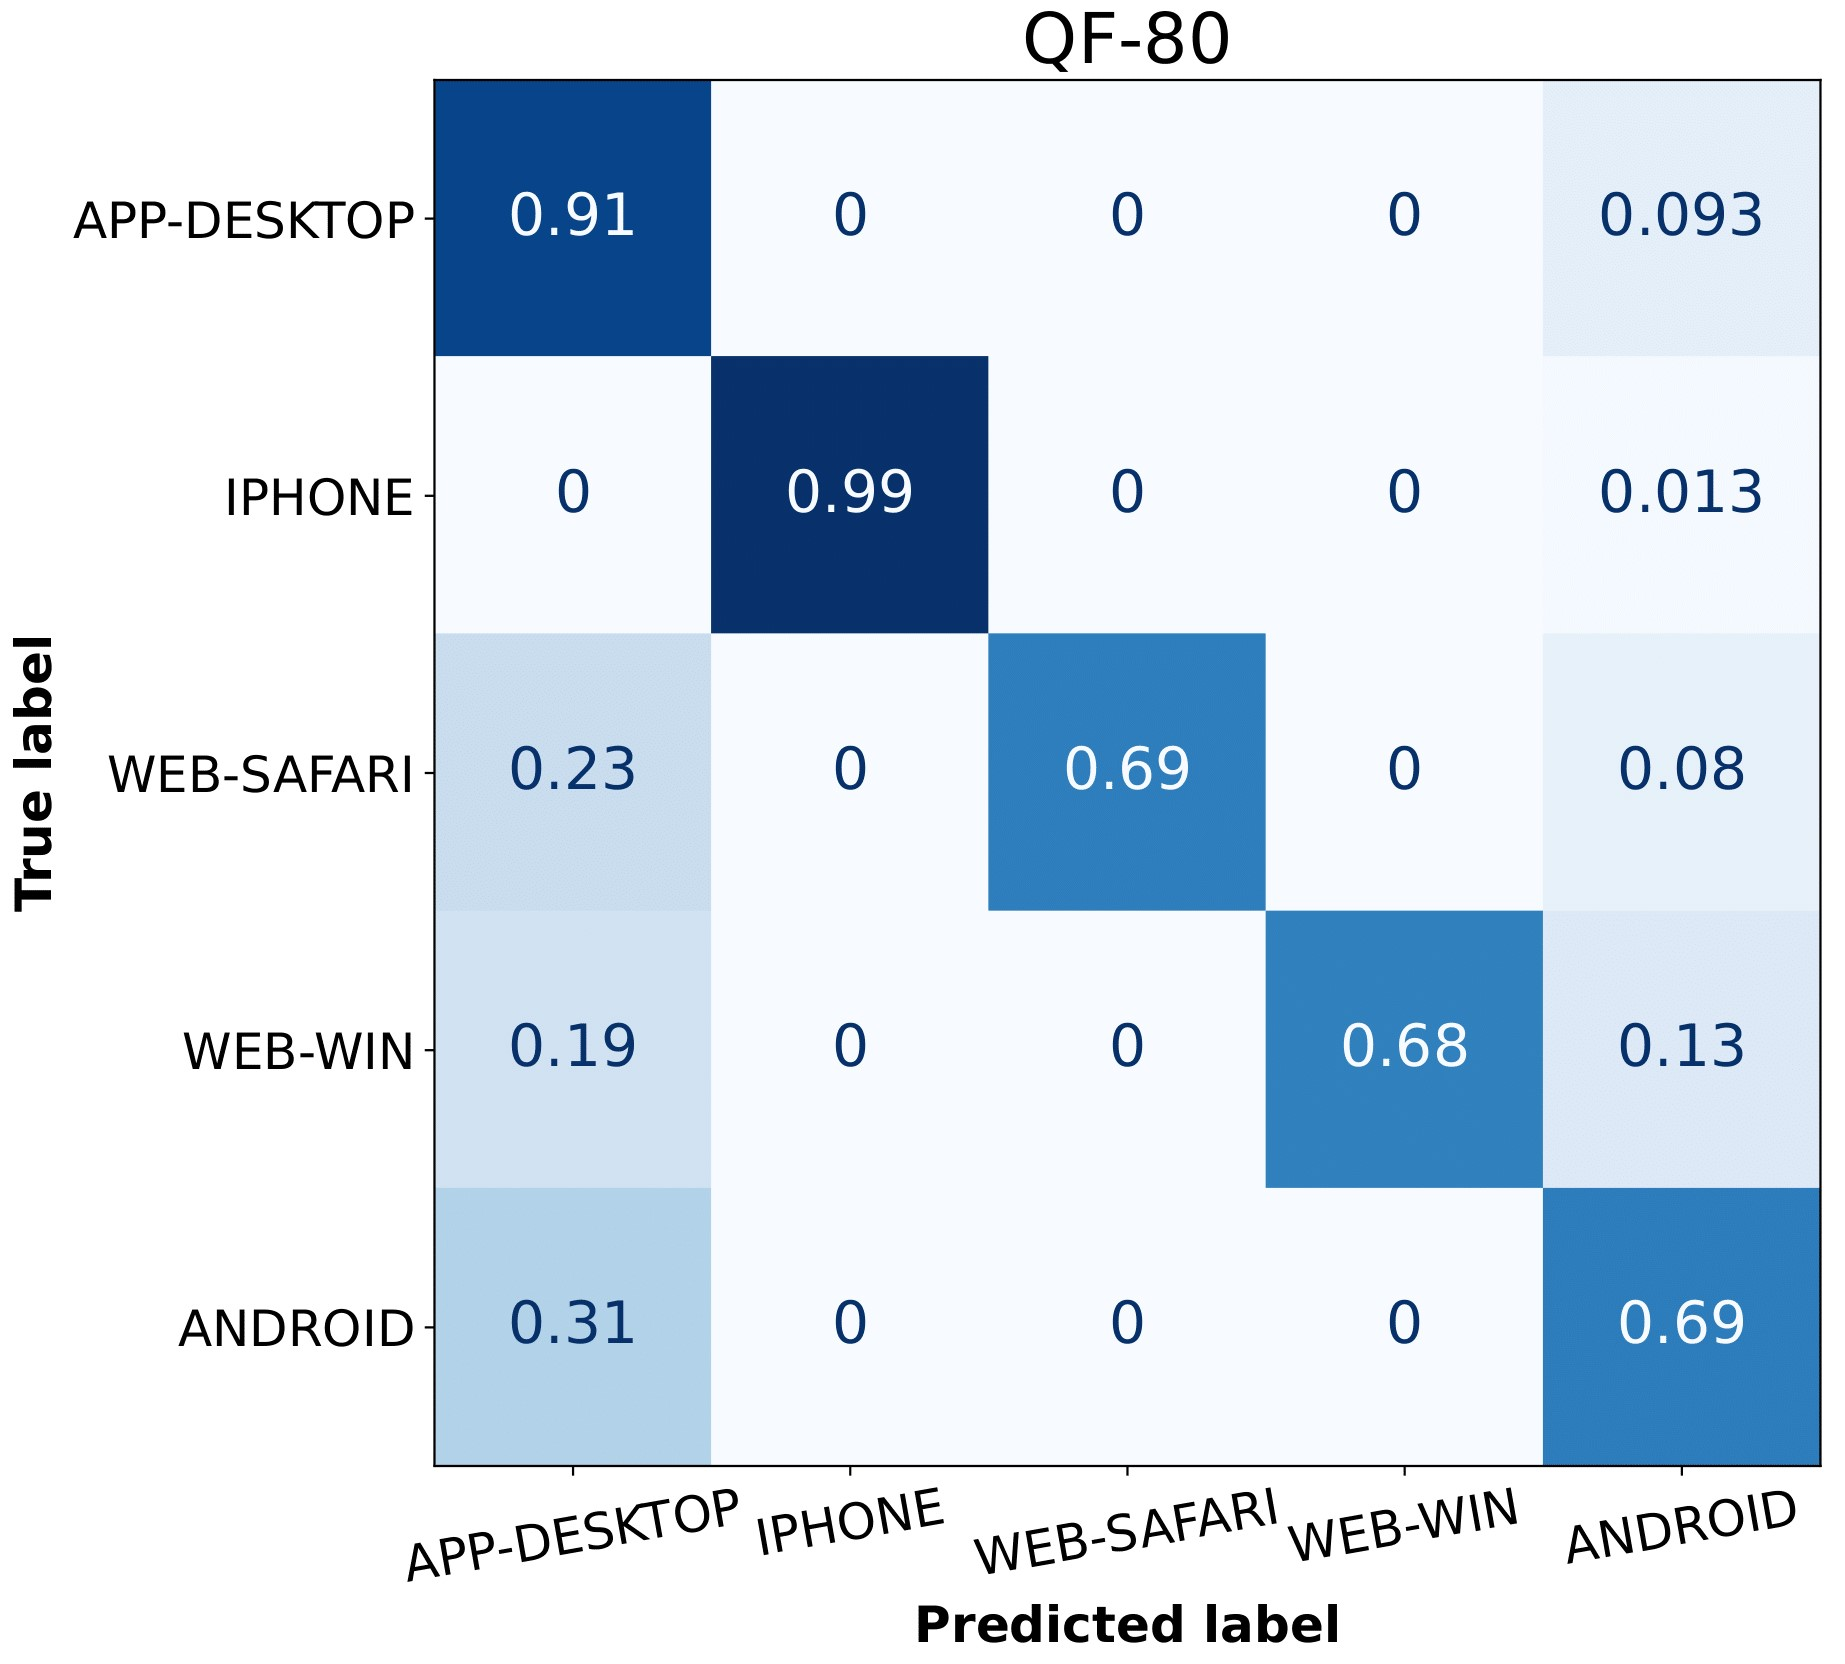
\includegraphics[width=8cm, height=8cm, keepaspectratio]{Immagini/Classificazione/confusion_matrix_SVM_QF-80.jpg}\\\vspace{1em}
    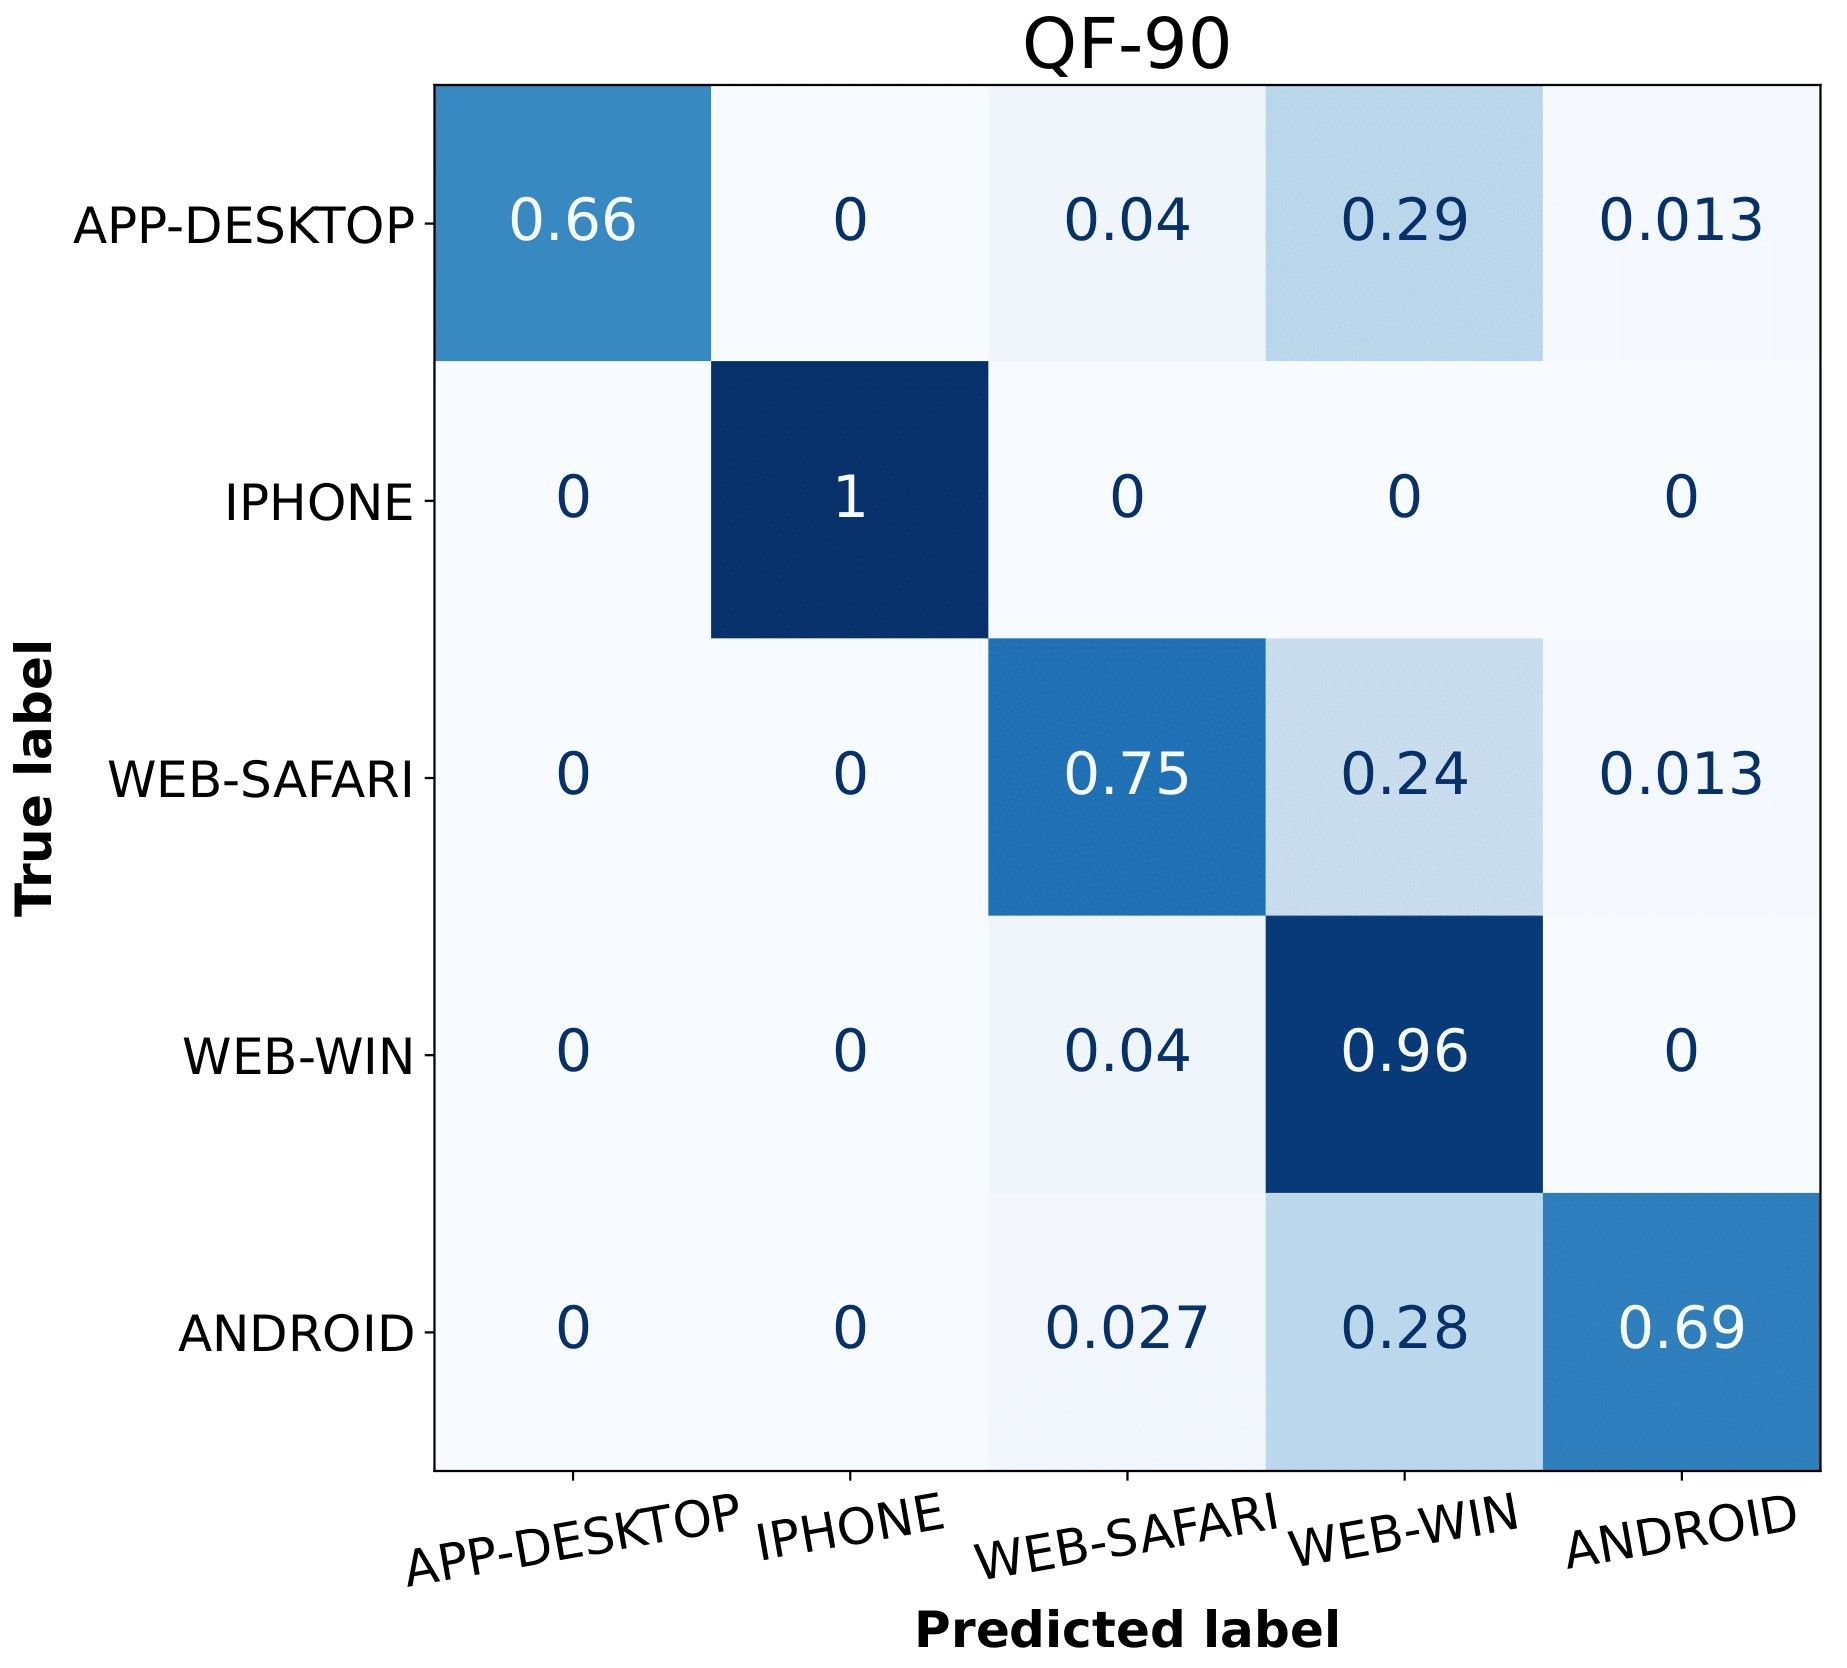
\includegraphics[width=8cm, height=8cm, keepaspectratio]{Immagini/Classificazione/confusion_matrix_SVM_QF-90.jpg}\ \ \ \ \
    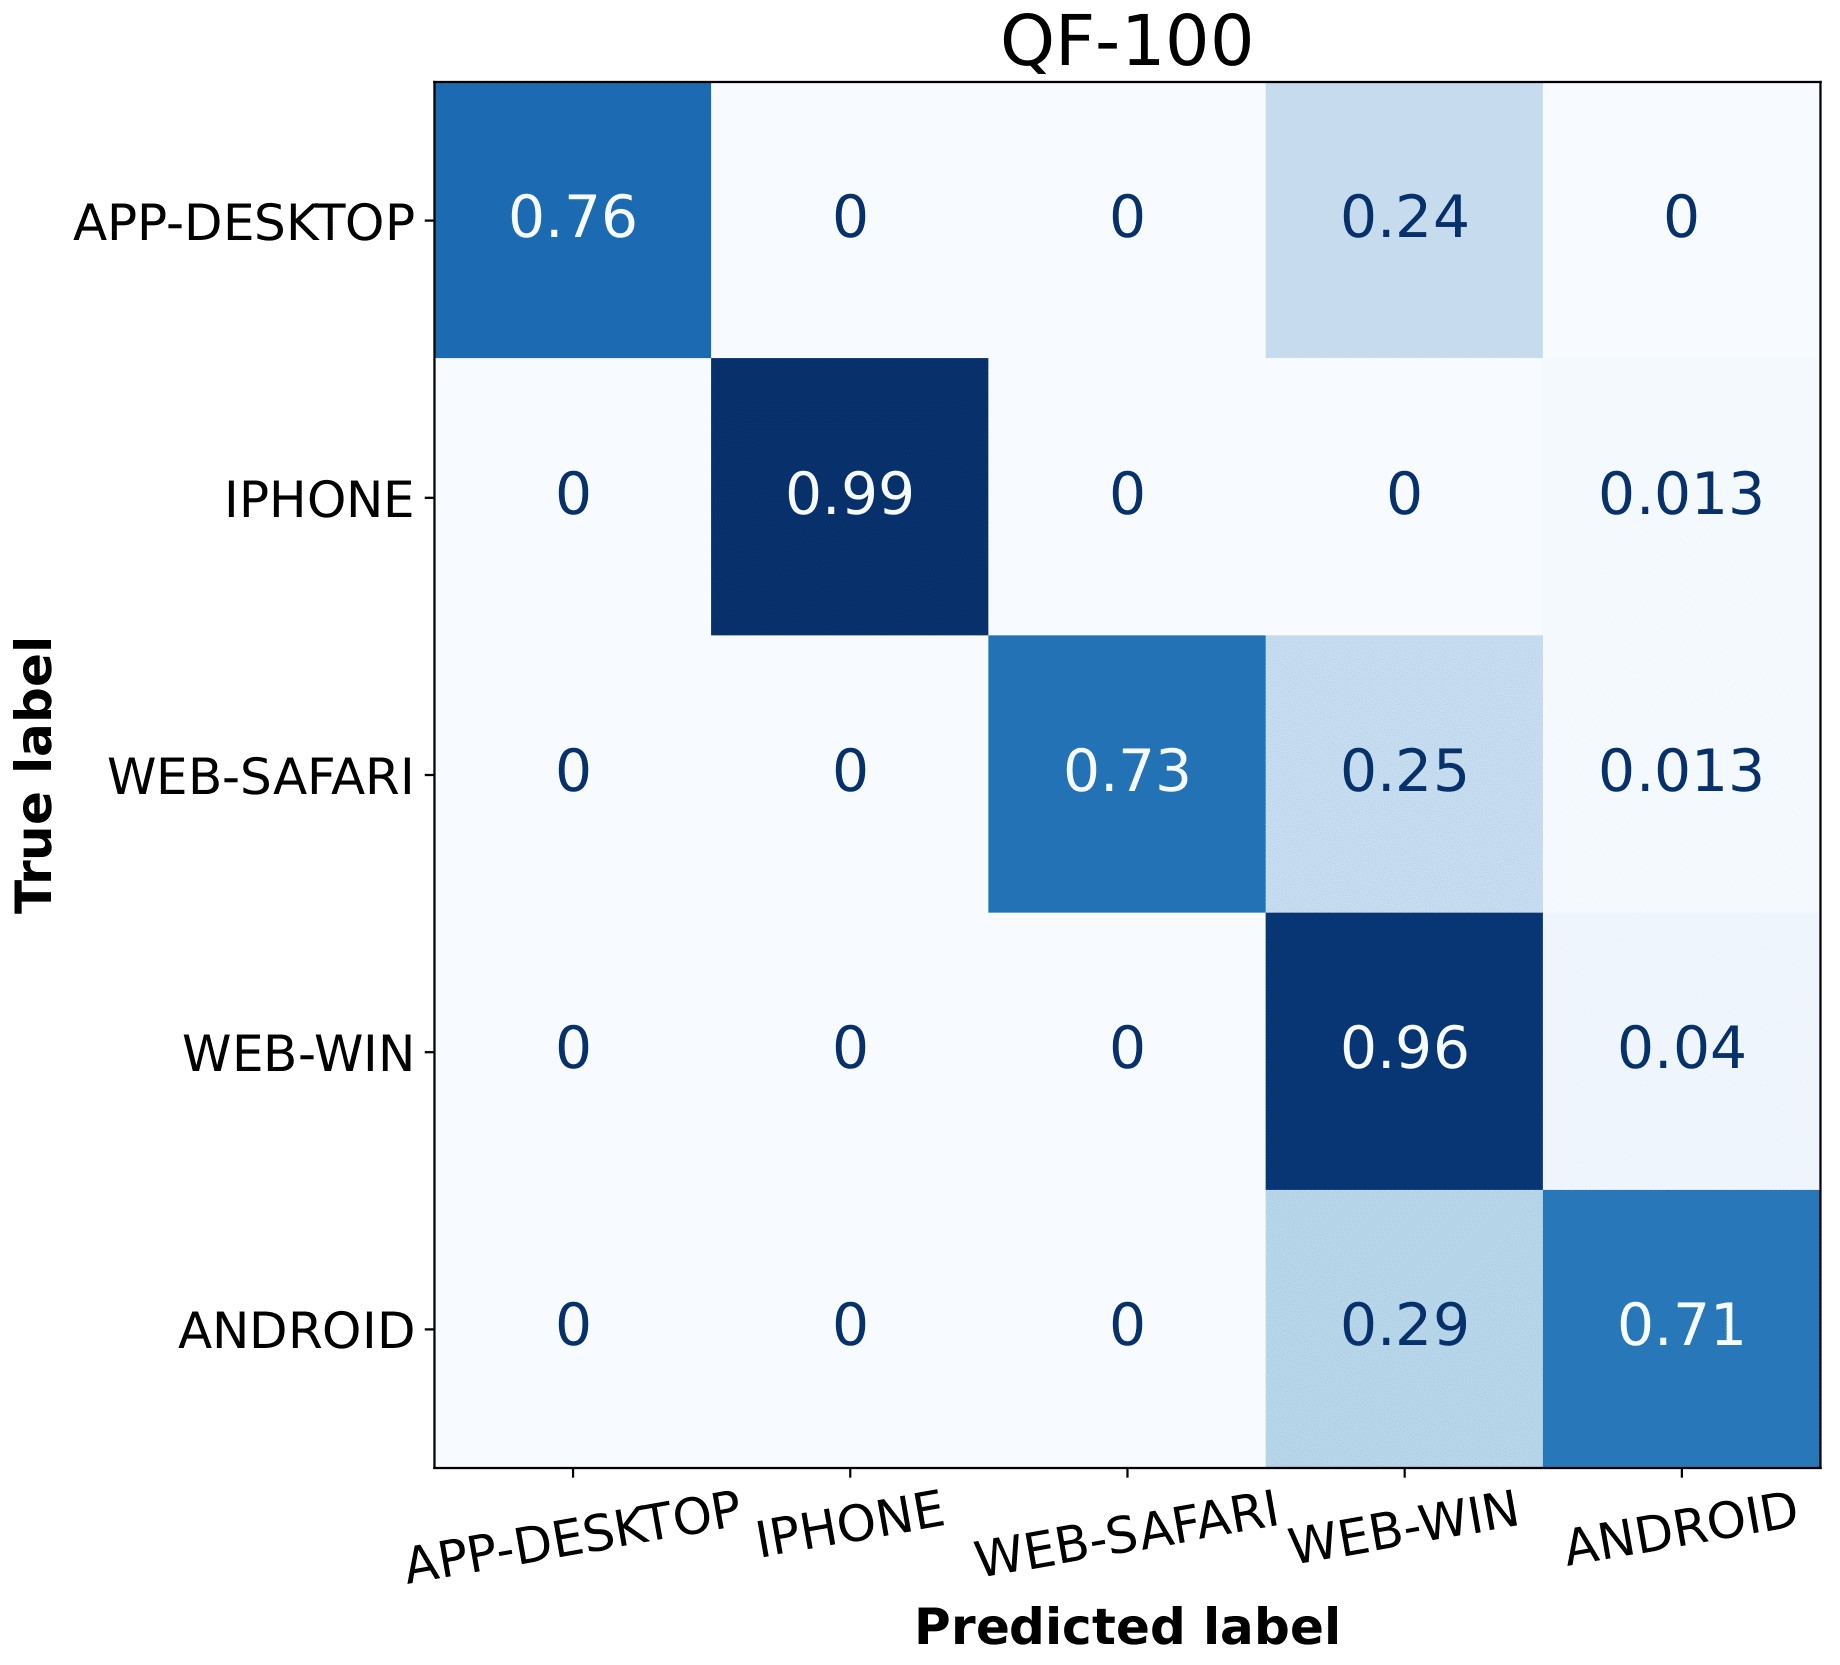
\includegraphics[width=8cm, height=8cm, keepaspectratio]{Immagini/Classificazione/confusion_matrix_SVM_QF-100.jpg}
    \captionof{figure}{\textit{Confusion matrix} per \textit{support vector machine} divise per \textit{quality factor}.}
    \label{fig:class_QF_SVM}
\endgroup

% \begin{figure}[h!]
%     \centering
%     \subfloat[][]{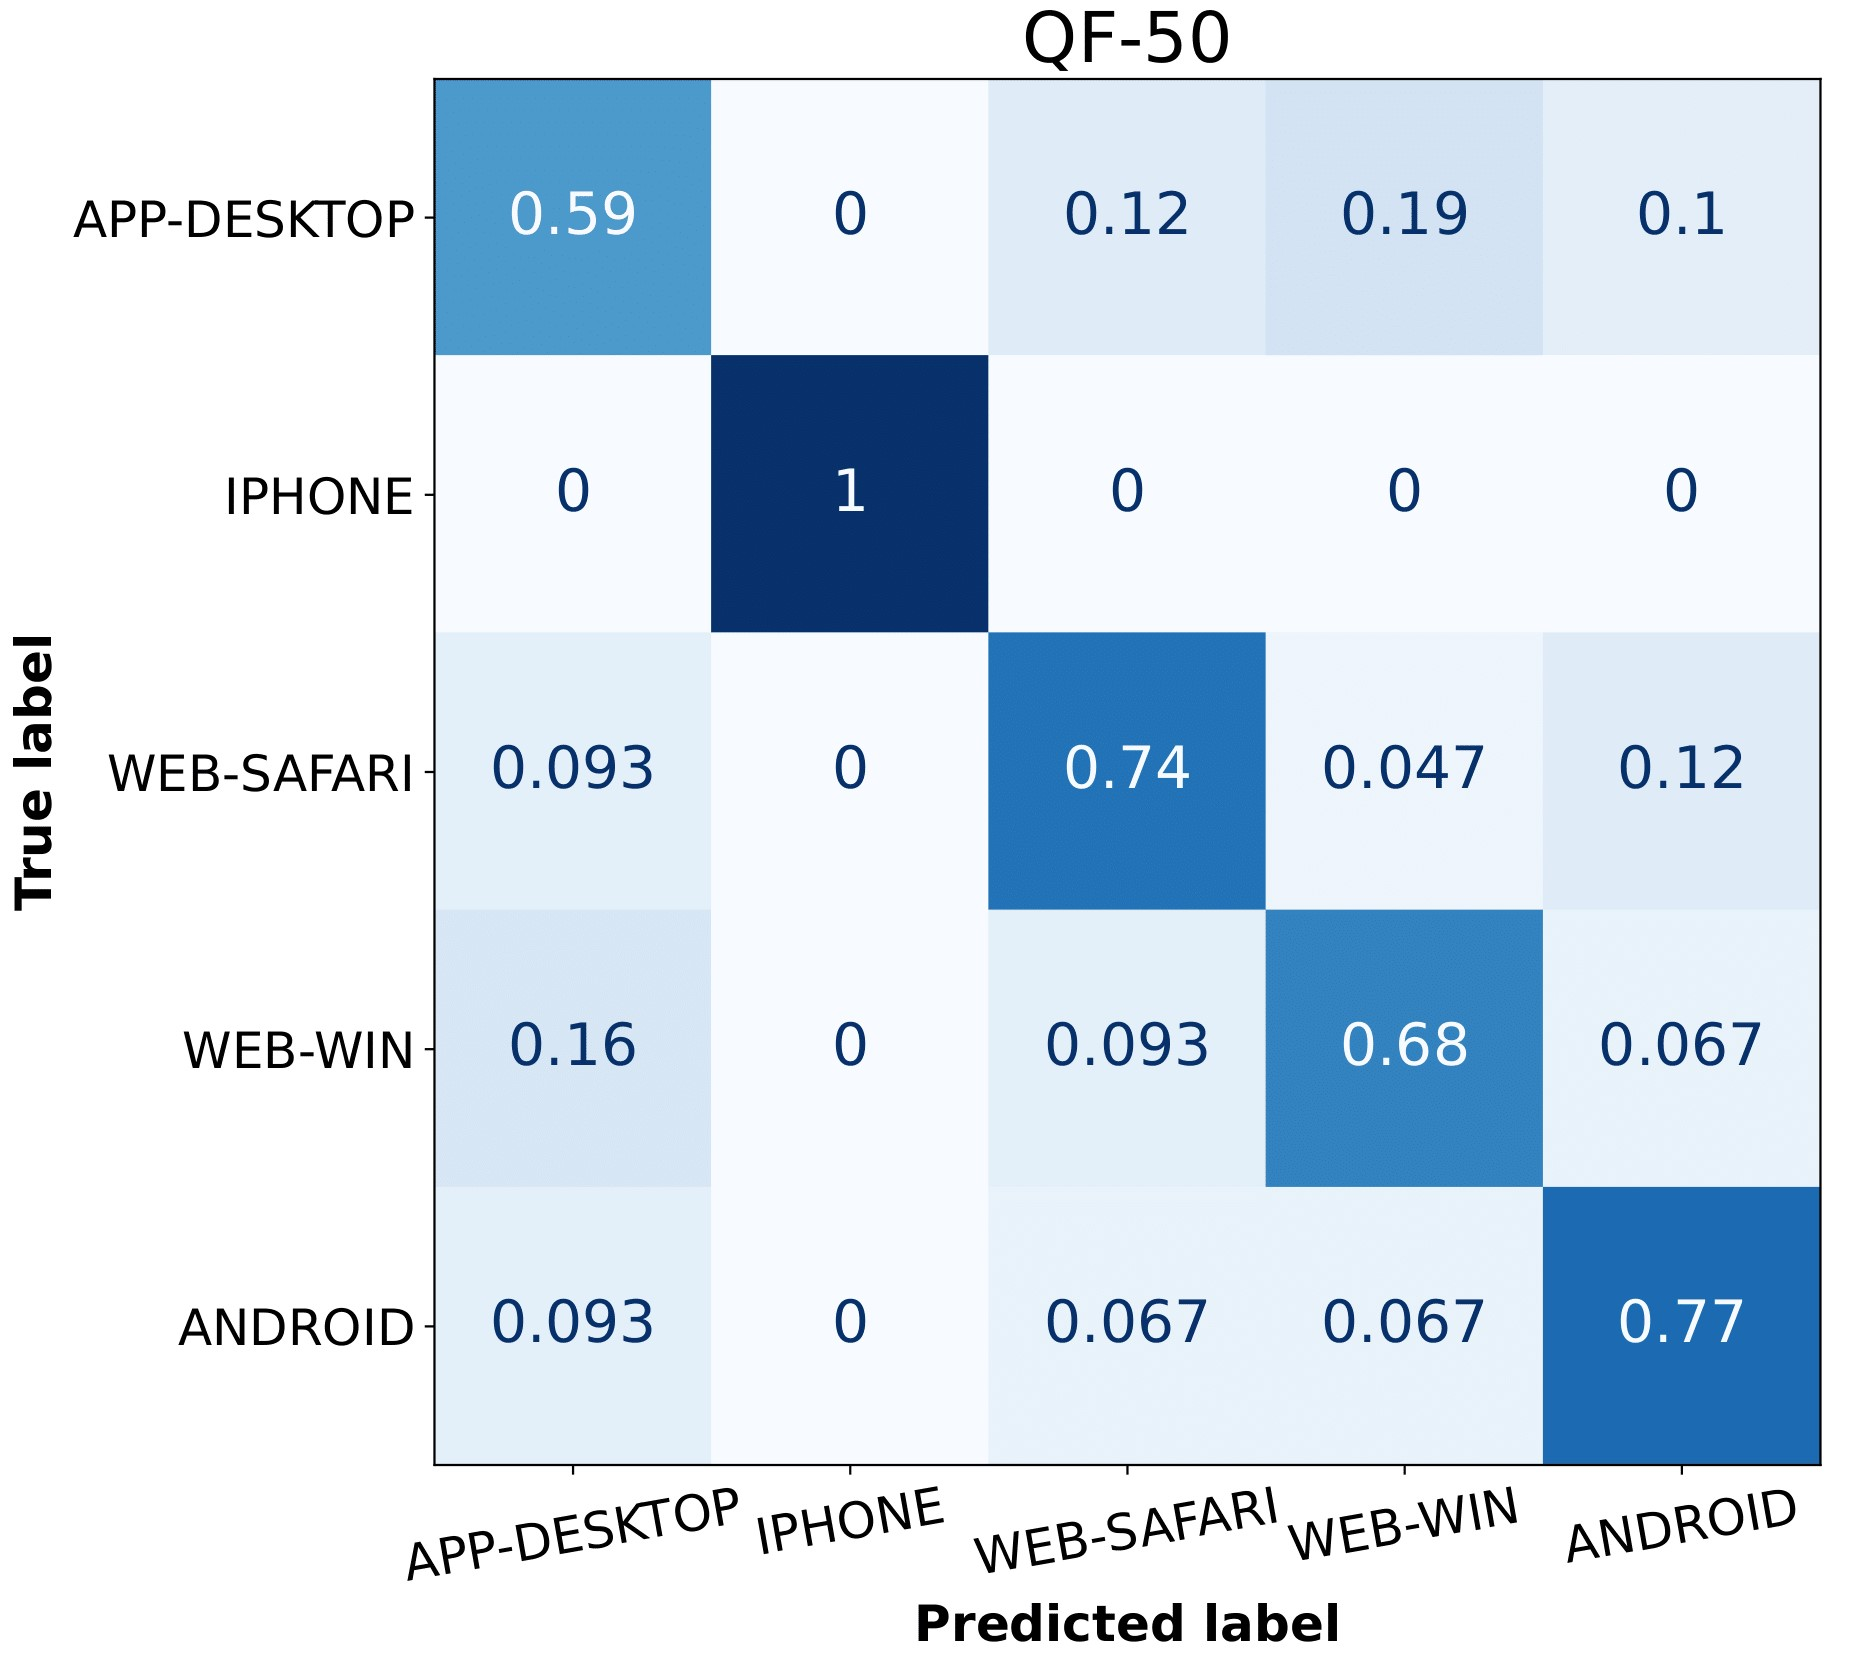
\includegraphics[width=8cm, height=8cm, keepaspectratio]{Immagini/Classificazione/confusion_matrix_RF_QF-50.jpg}}\ \ \ \ \
%     \subfloat[][]{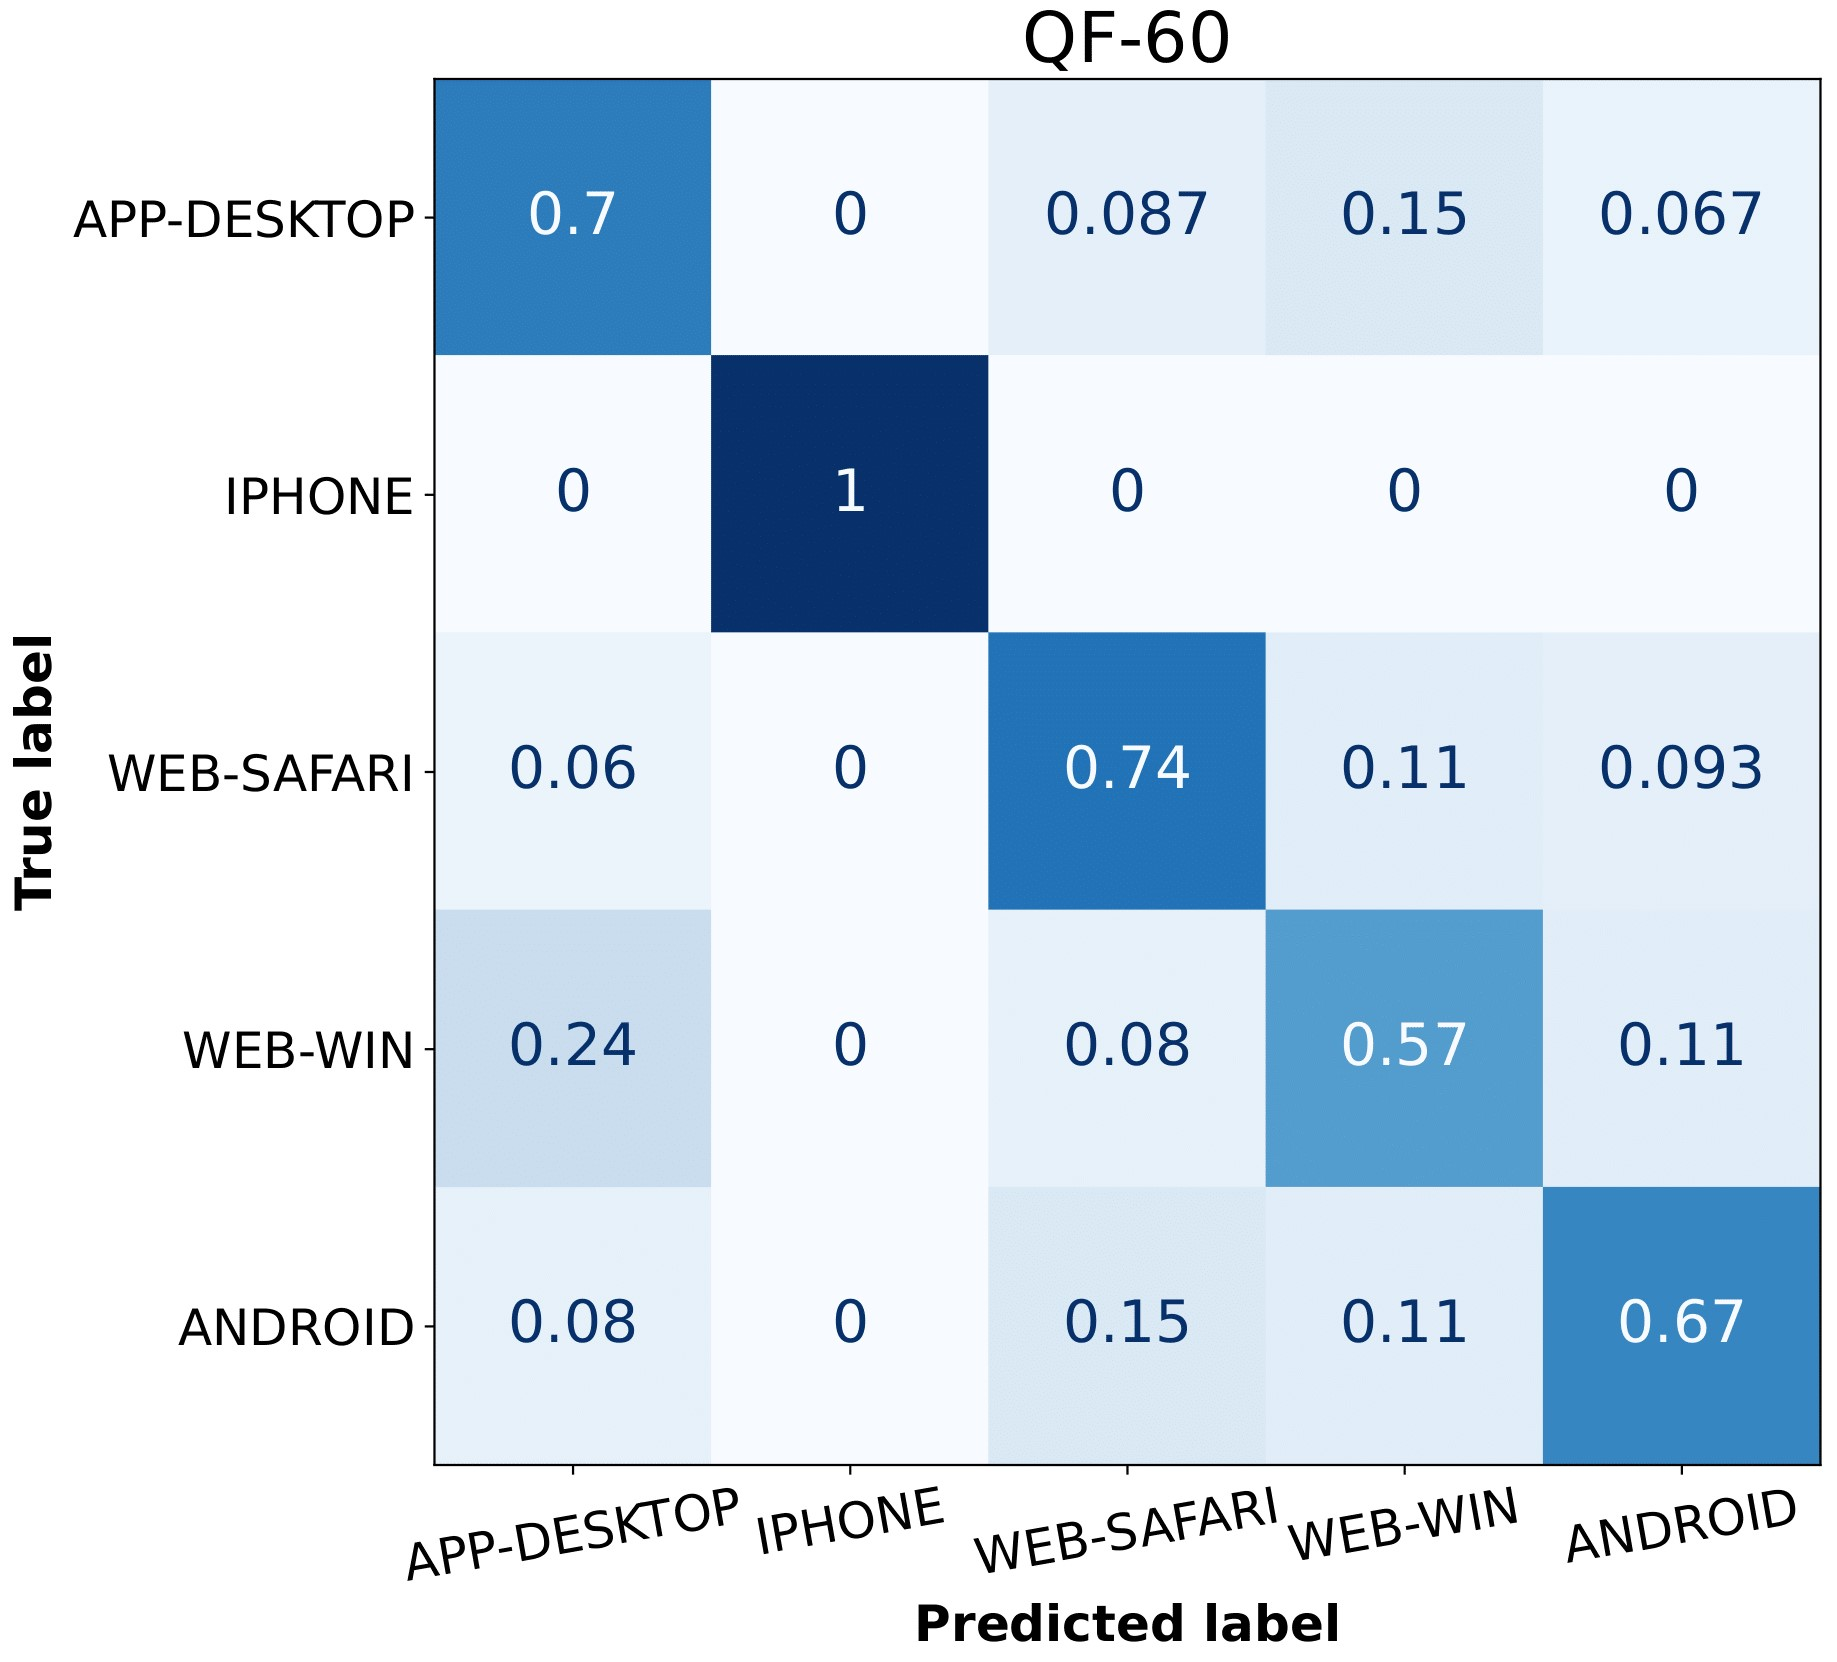
\includegraphics[width=8cm, height=8cm, keepaspectratio]{Immagini/Classificazione/confusion_matrix_RF_QF-60.jpg}}\\
%     \subfloat[][]{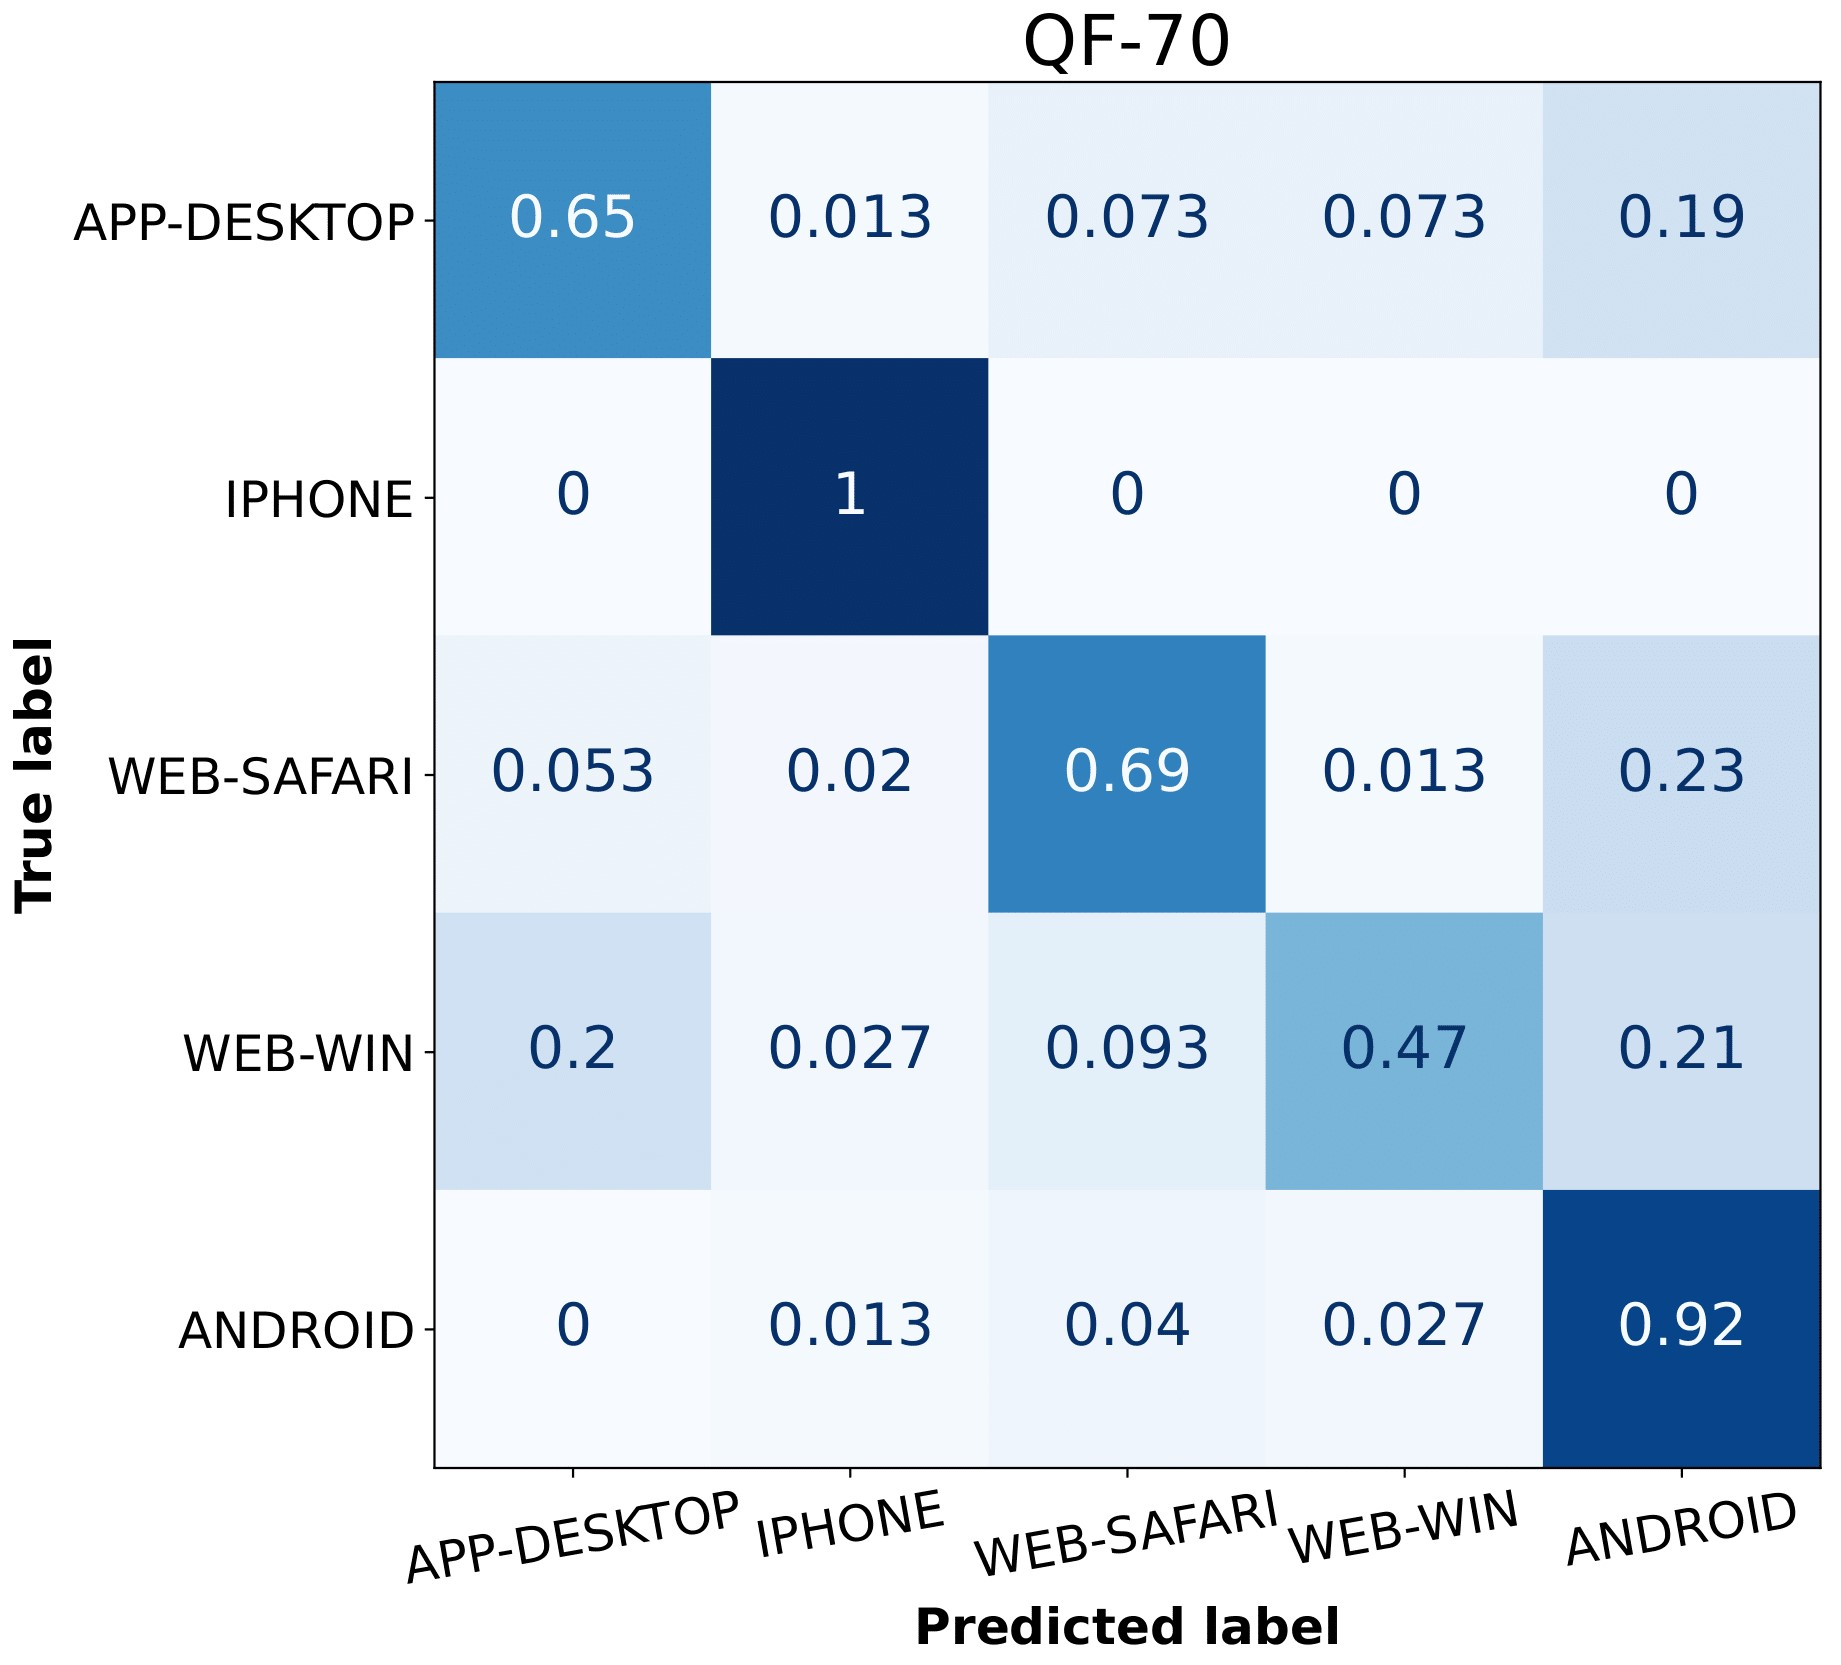
\includegraphics[width=8cm, height=8cm, keepaspectratio]{Immagini/Classificazione/confusion_matrix_RF_QF-70.jpg}}\ \ \ \ \
%     \subfloat[][]{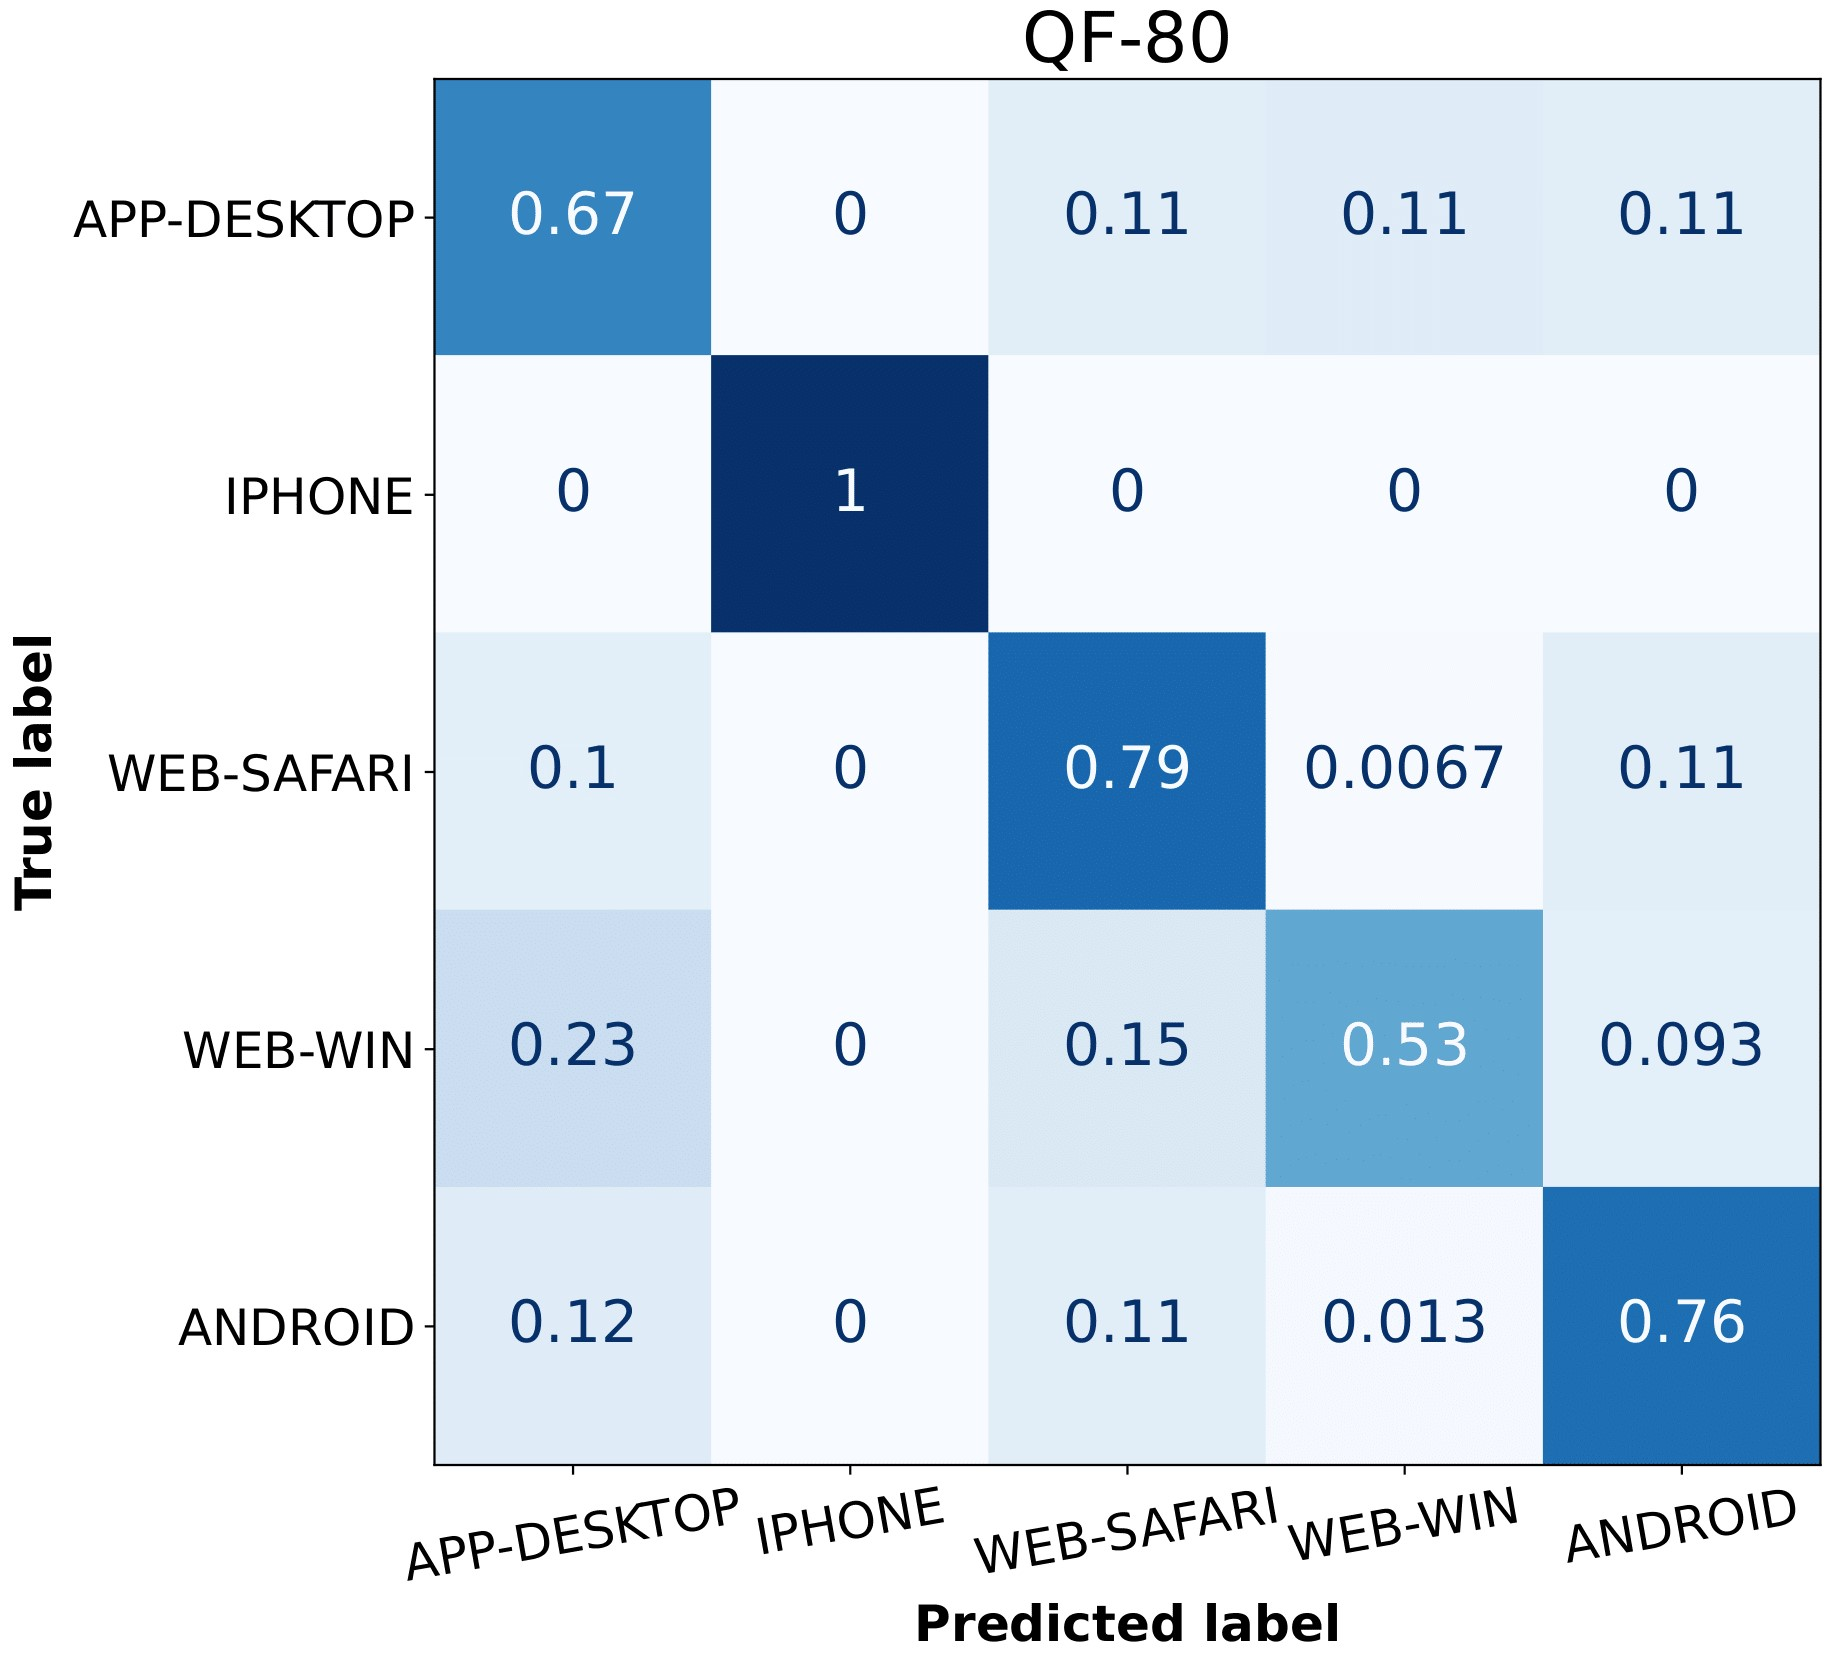
\includegraphics[width=8cm, height=8cm, keepaspectratio]{Immagini/Classificazione/confusion_matrix_RF_QF-80.jpg}}\\
%     \subfloat[][]{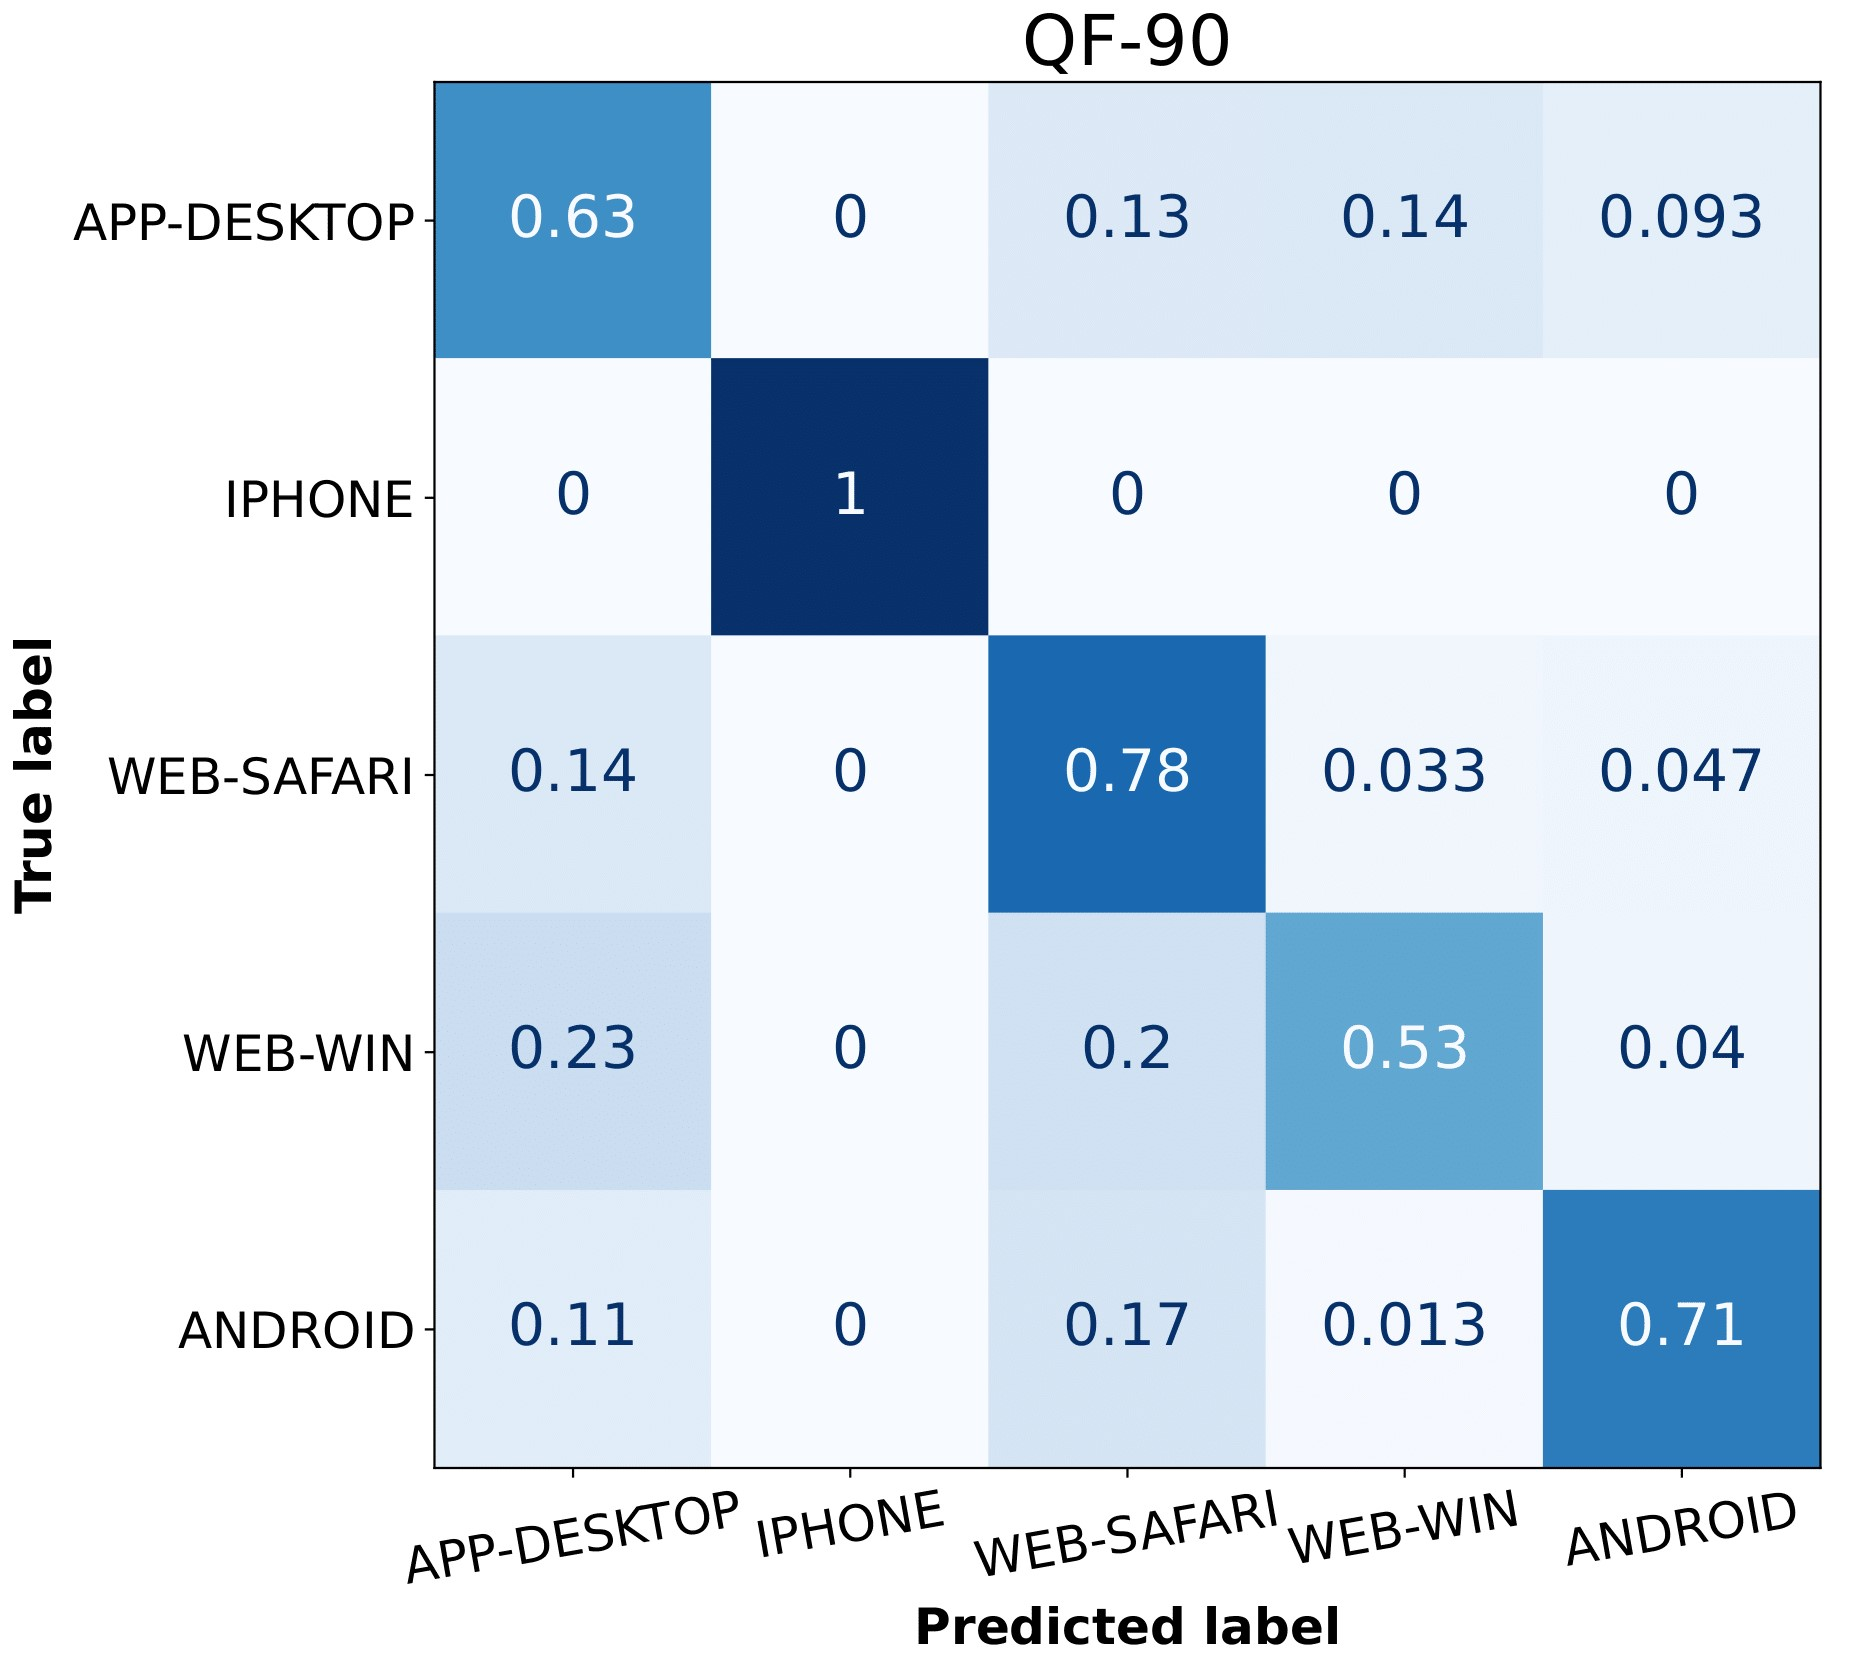
\includegraphics[width=8cm, height=8cm, keepaspectratio]{Immagini/Classificazione/confusion_matrix_RF_QF-90.jpg}}\ \ \ \ \
%     \subfloat[][]{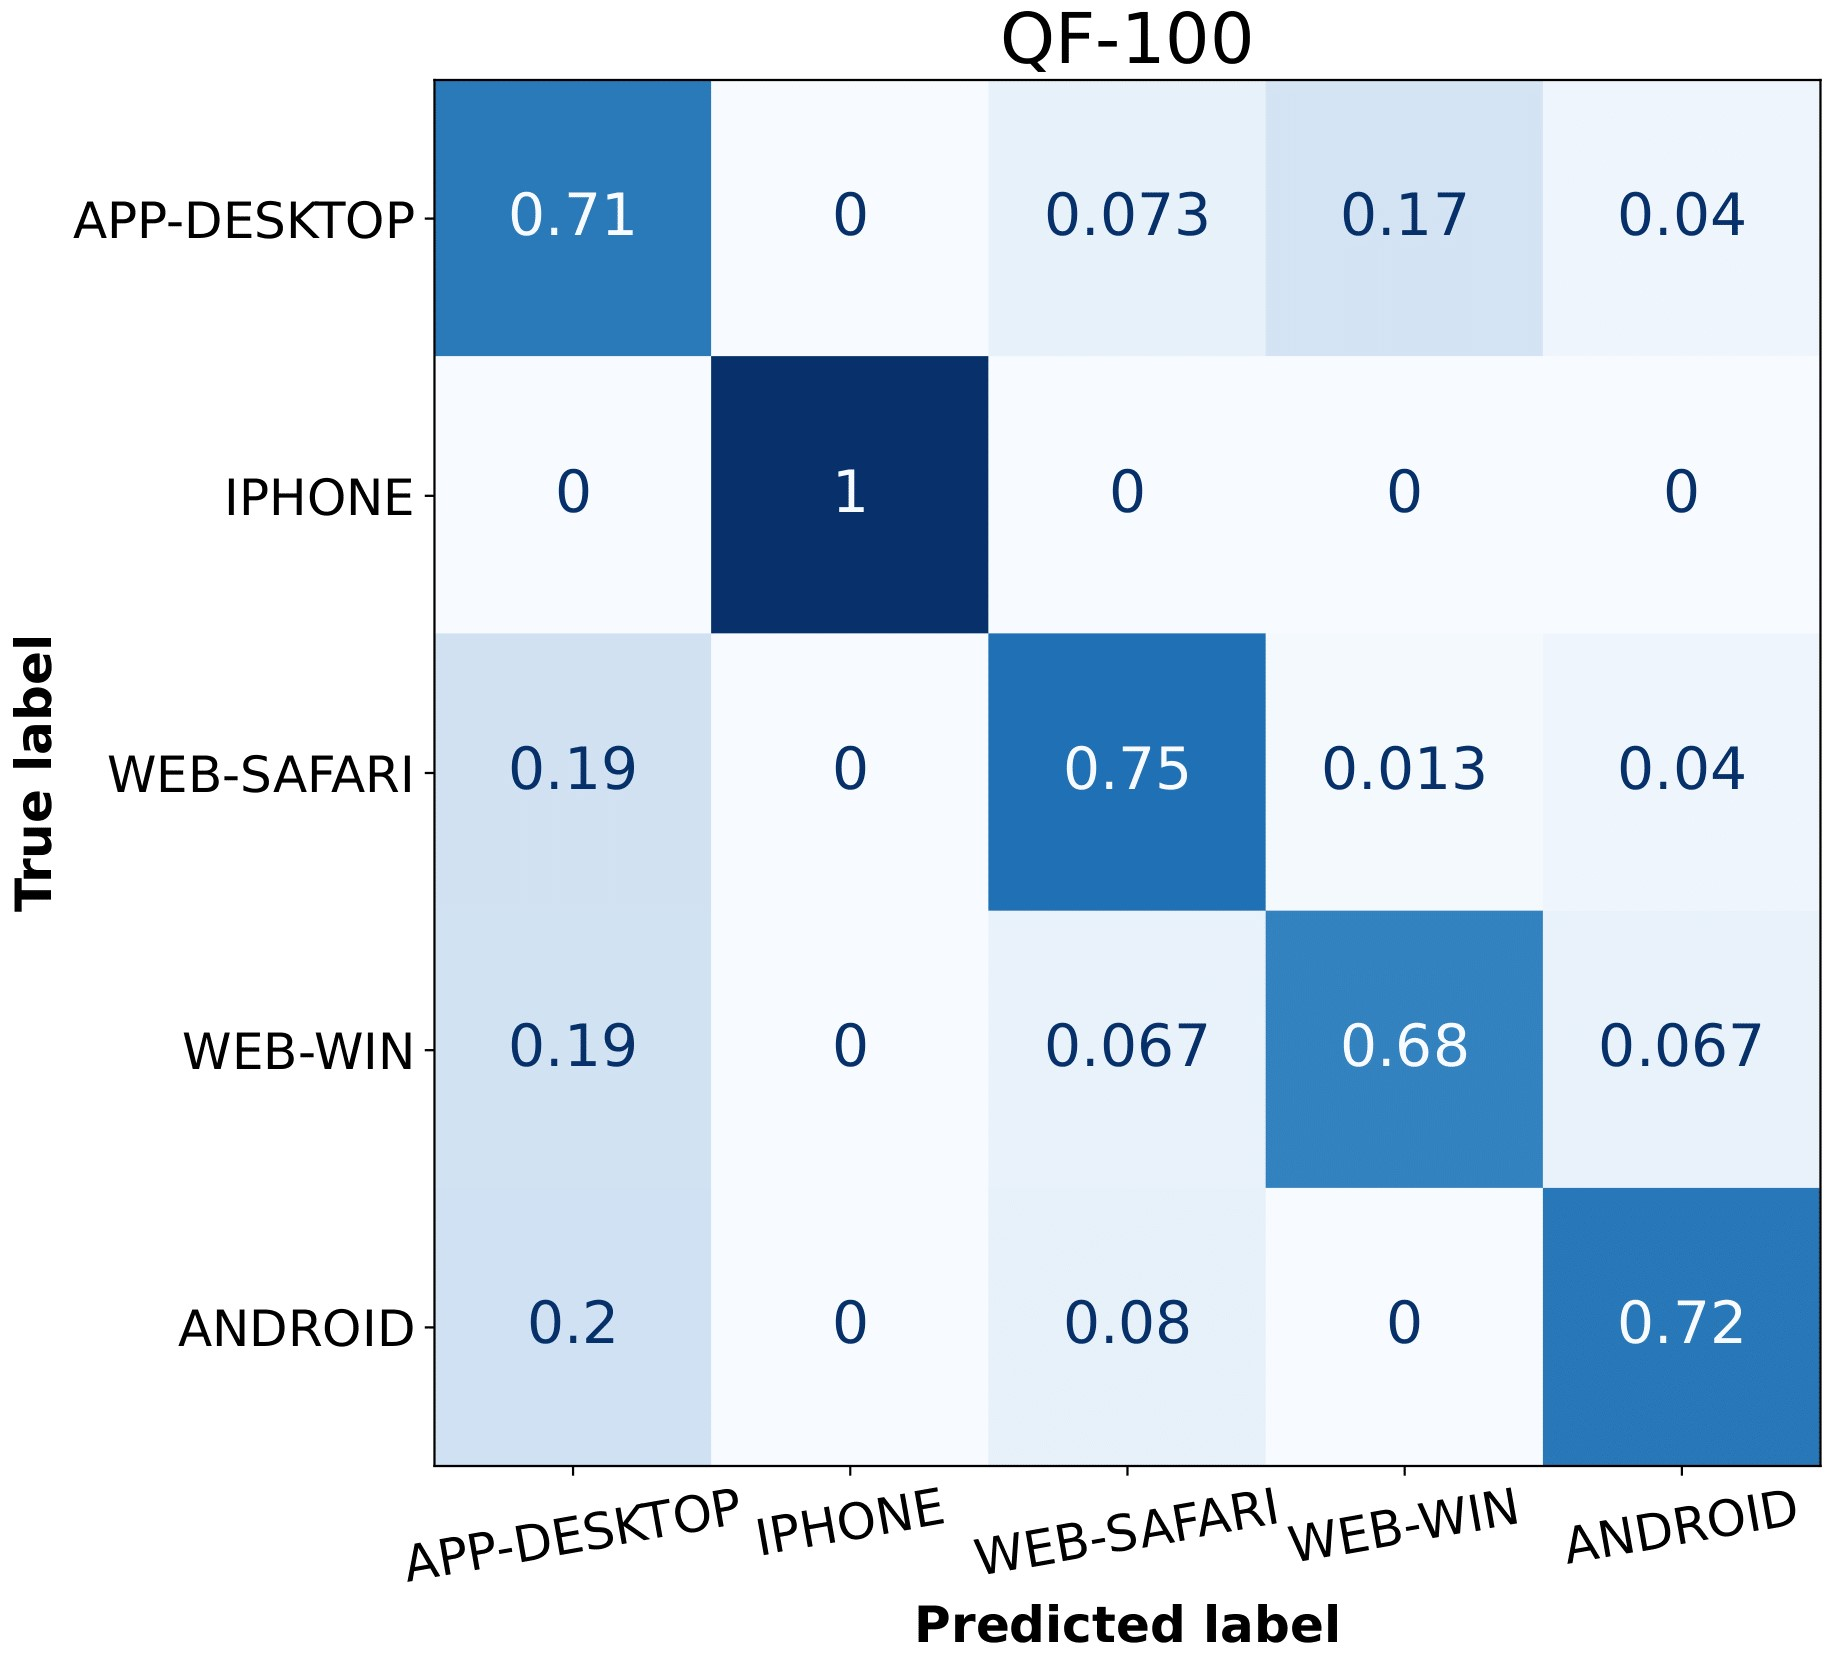
\includegraphics[width=8cm, height=8cm, keepaspectratio]{Immagini/Classificazione/confusion_matrix_RF_QF-100.jpg}}
%     \caption{\textit{Confusion matrix} per \textit{random forest} divise per \textit{quality factor}.}
%     \label{fig:class_QF_RF}
% \end{figure}

% \begin{figure}[h!]
%     \centering
%     \subfloat[][]{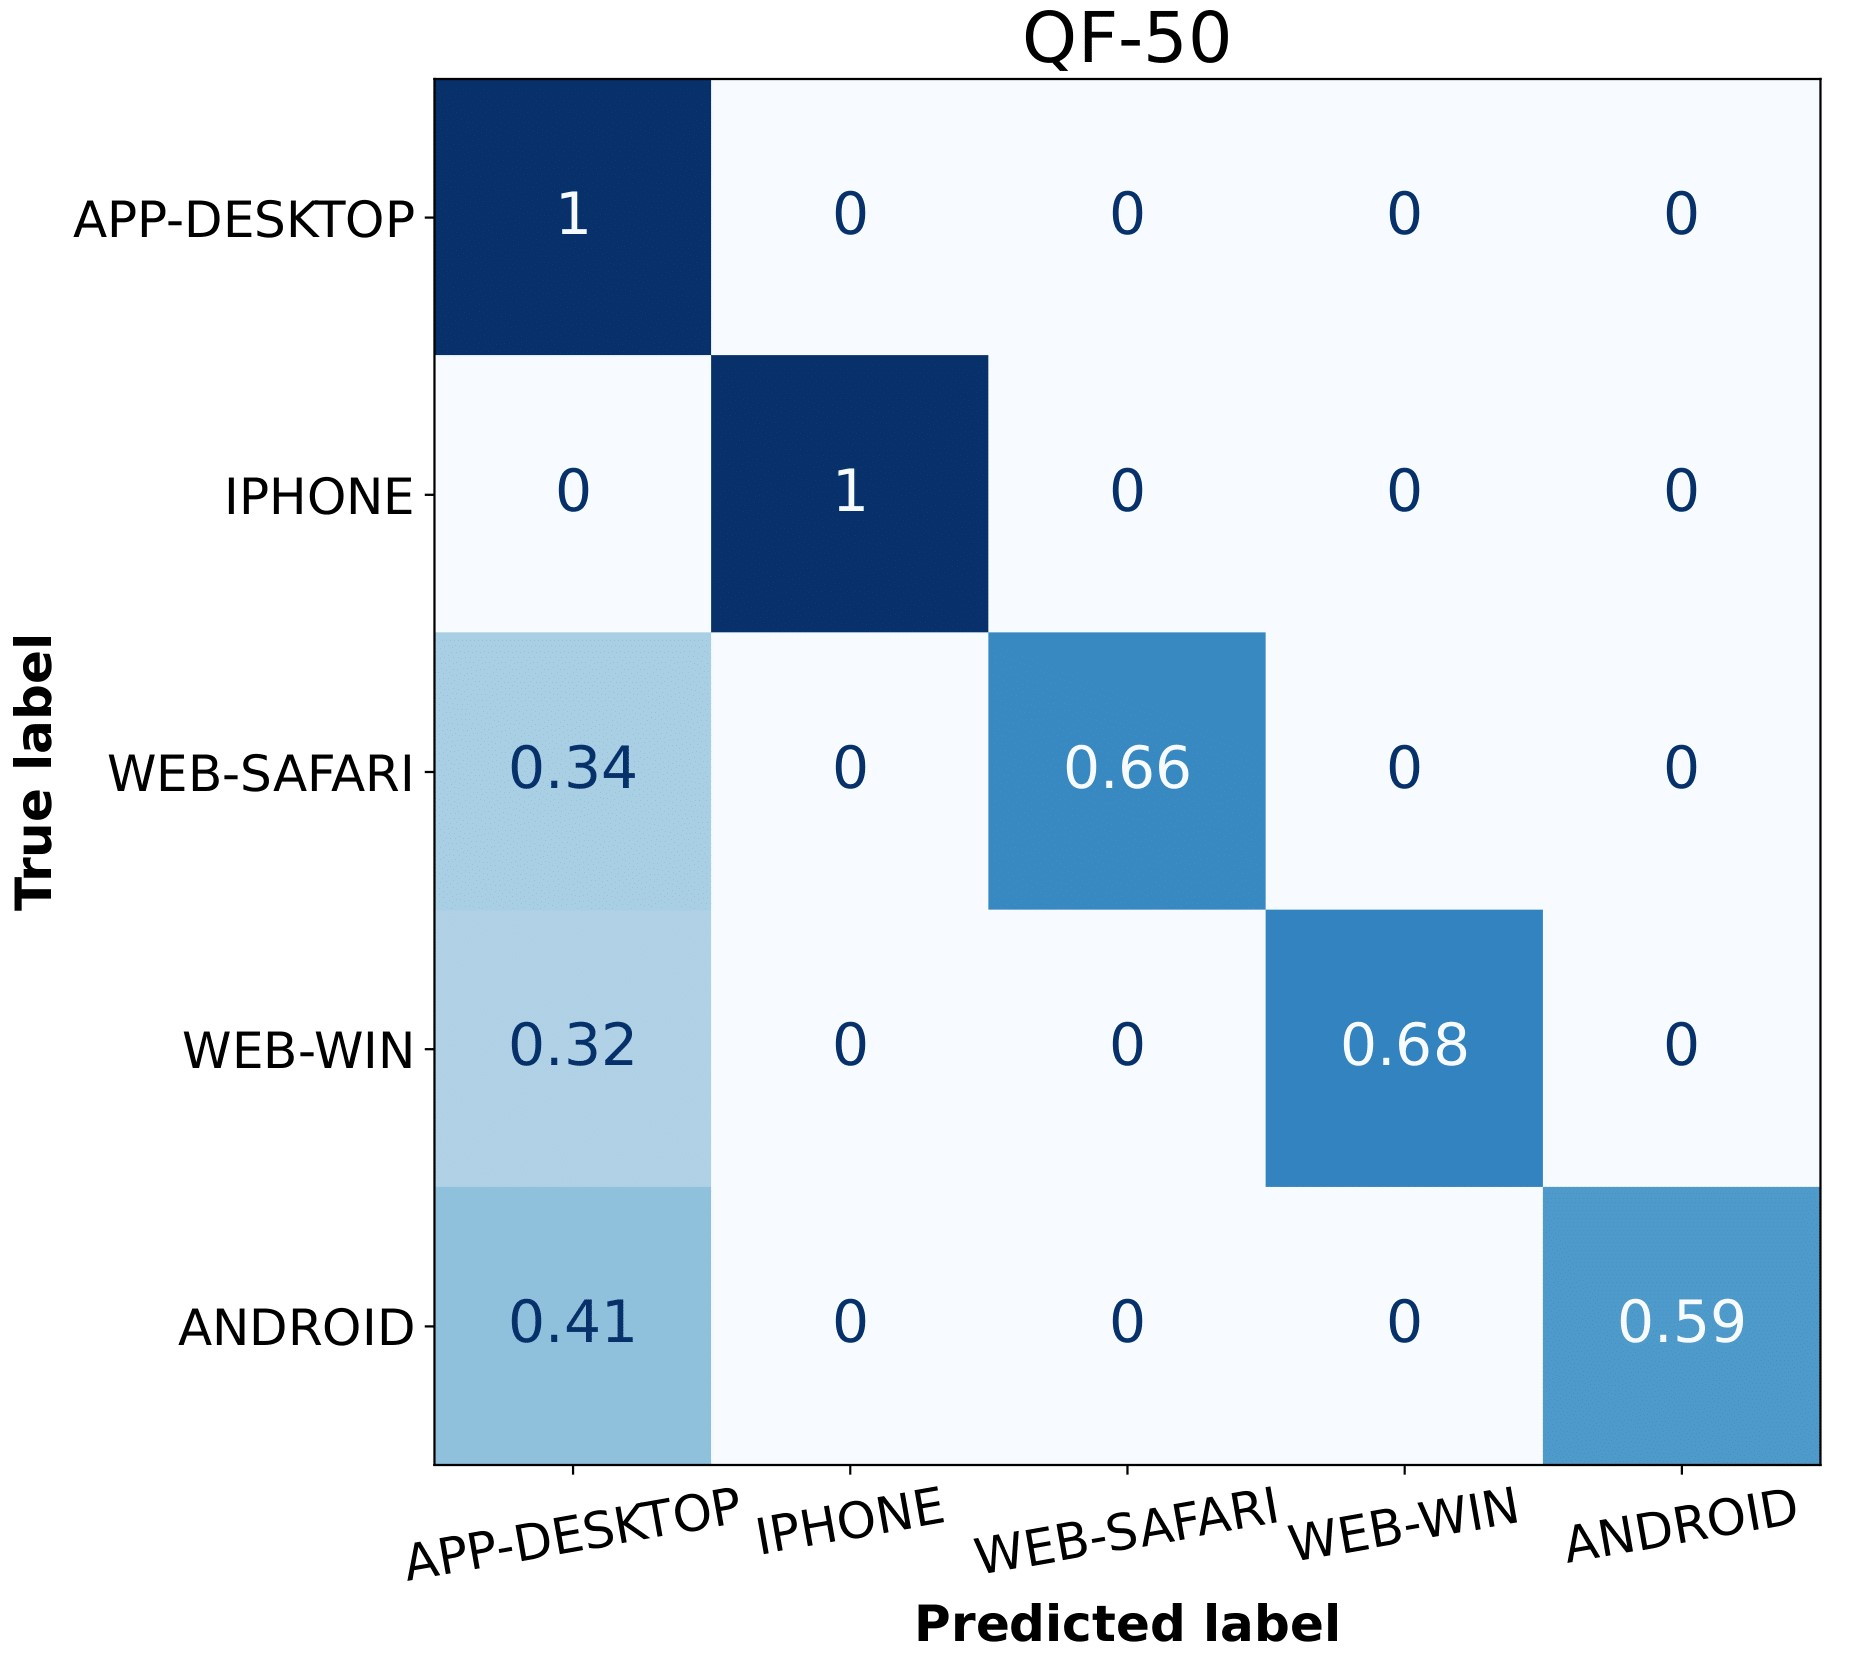
\includegraphics[width=8cm, height=8cm, keepaspectratio]{Immagini/Classificazione/confusion_matrix_SVM_QF-50.jpg}}\ \ \ \ \
%     \subfloat[][]{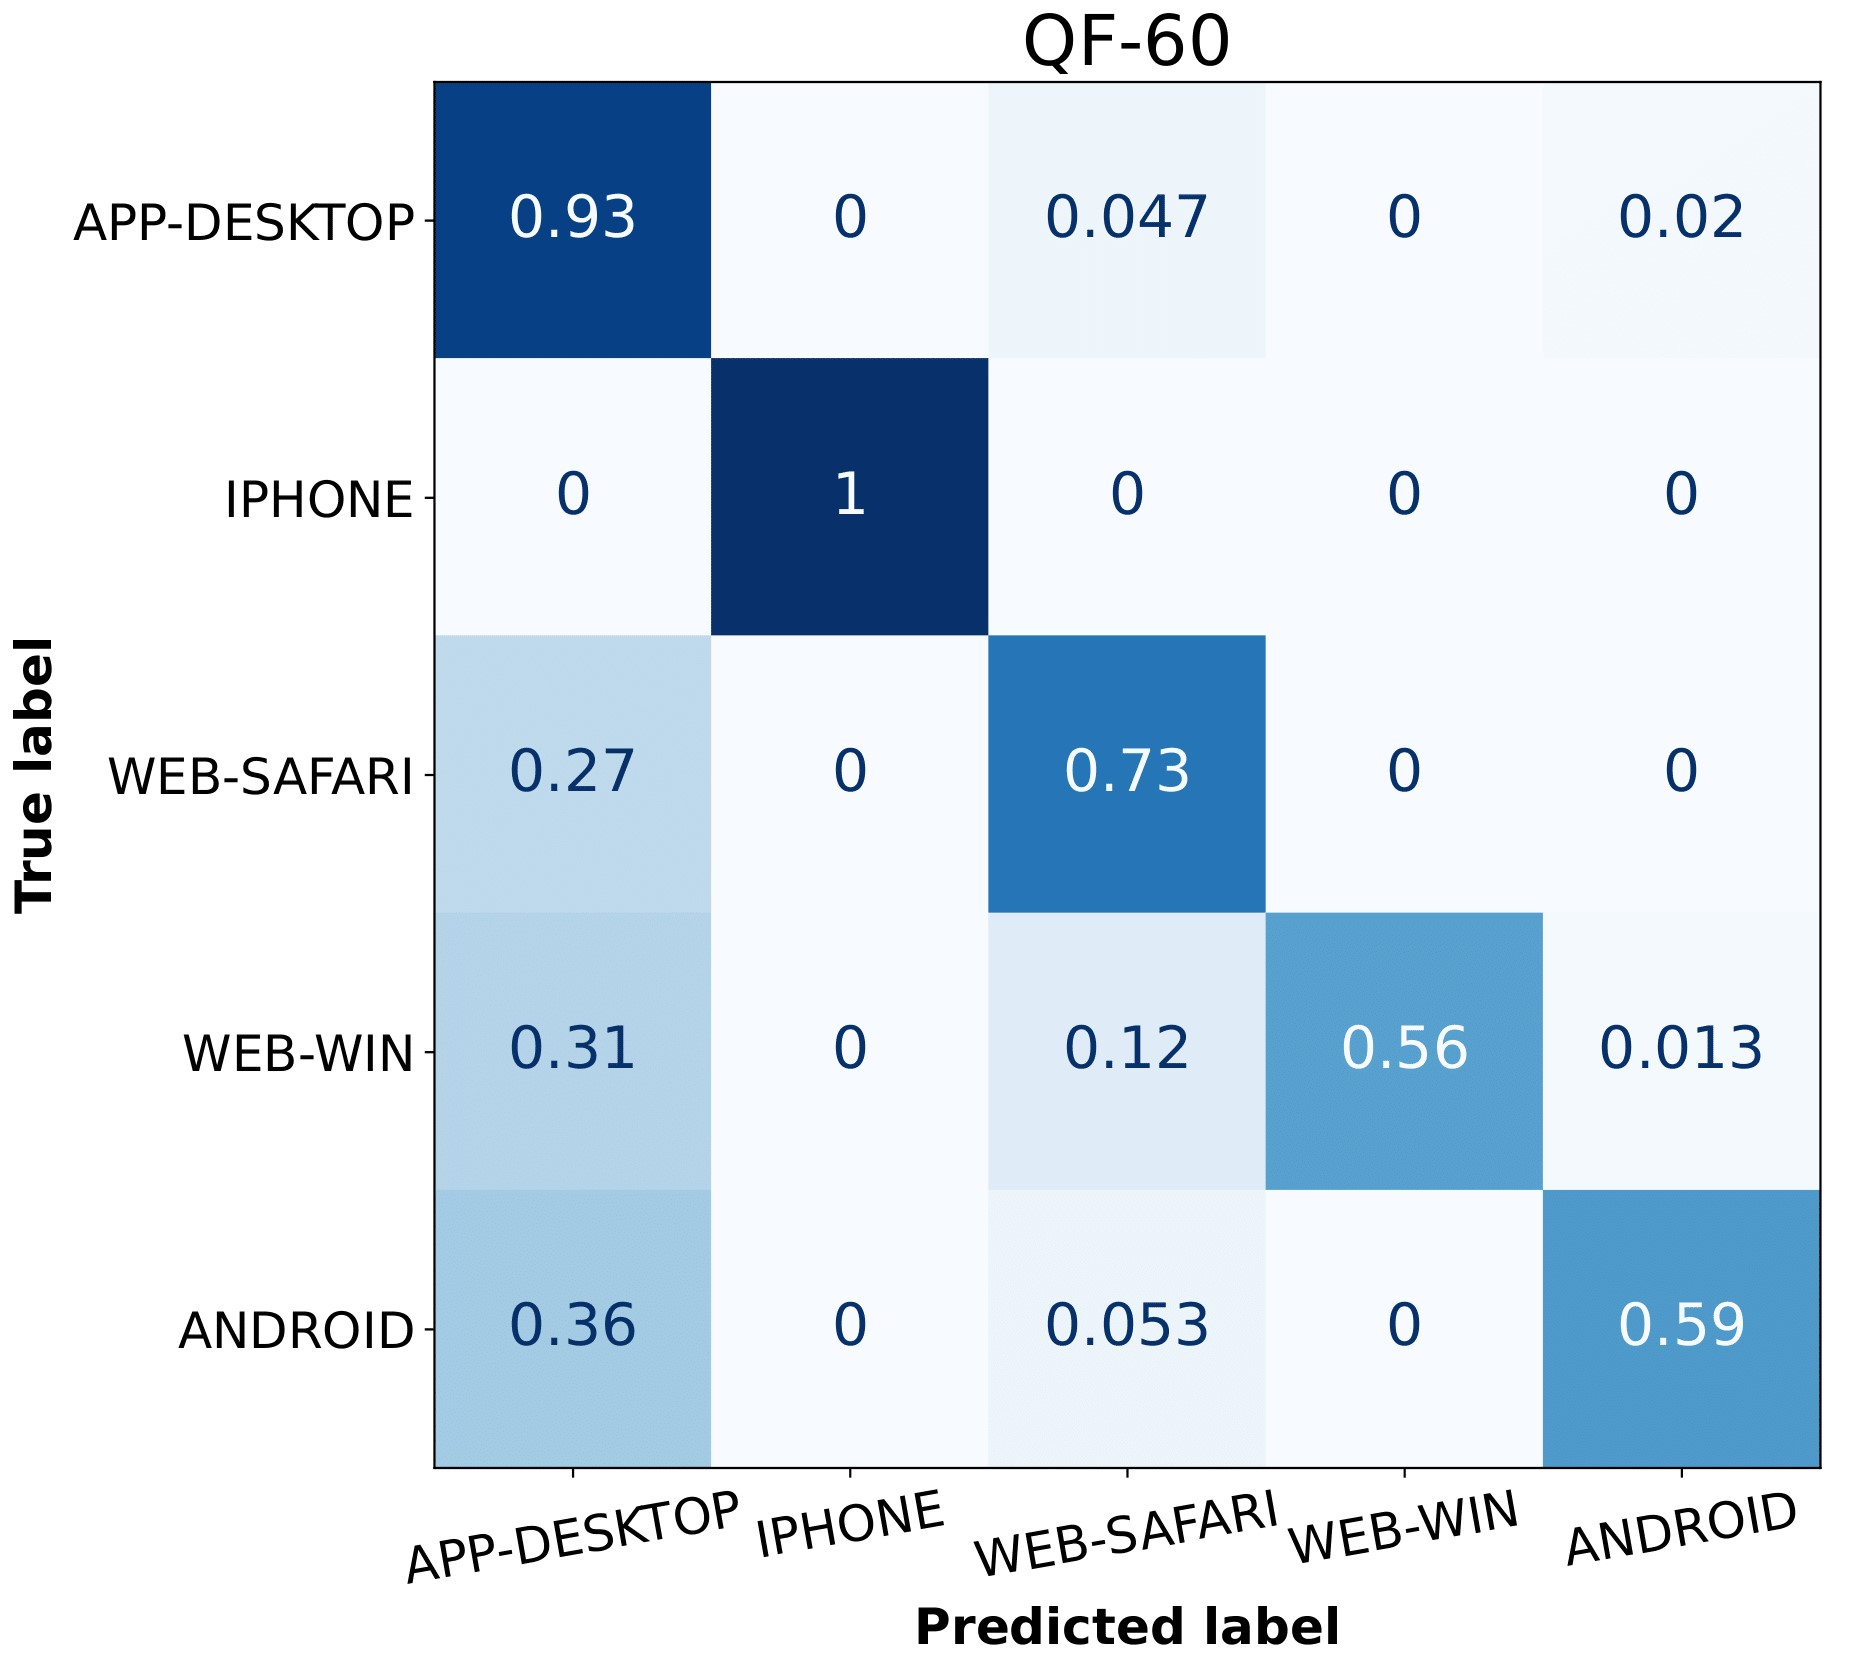
\includegraphics[width=8cm, height=8cm, keepaspectratio]{Immagini/Classificazione/confusion_matrix_SVM_QF-60.jpg}}\\
%     \subfloat[][]{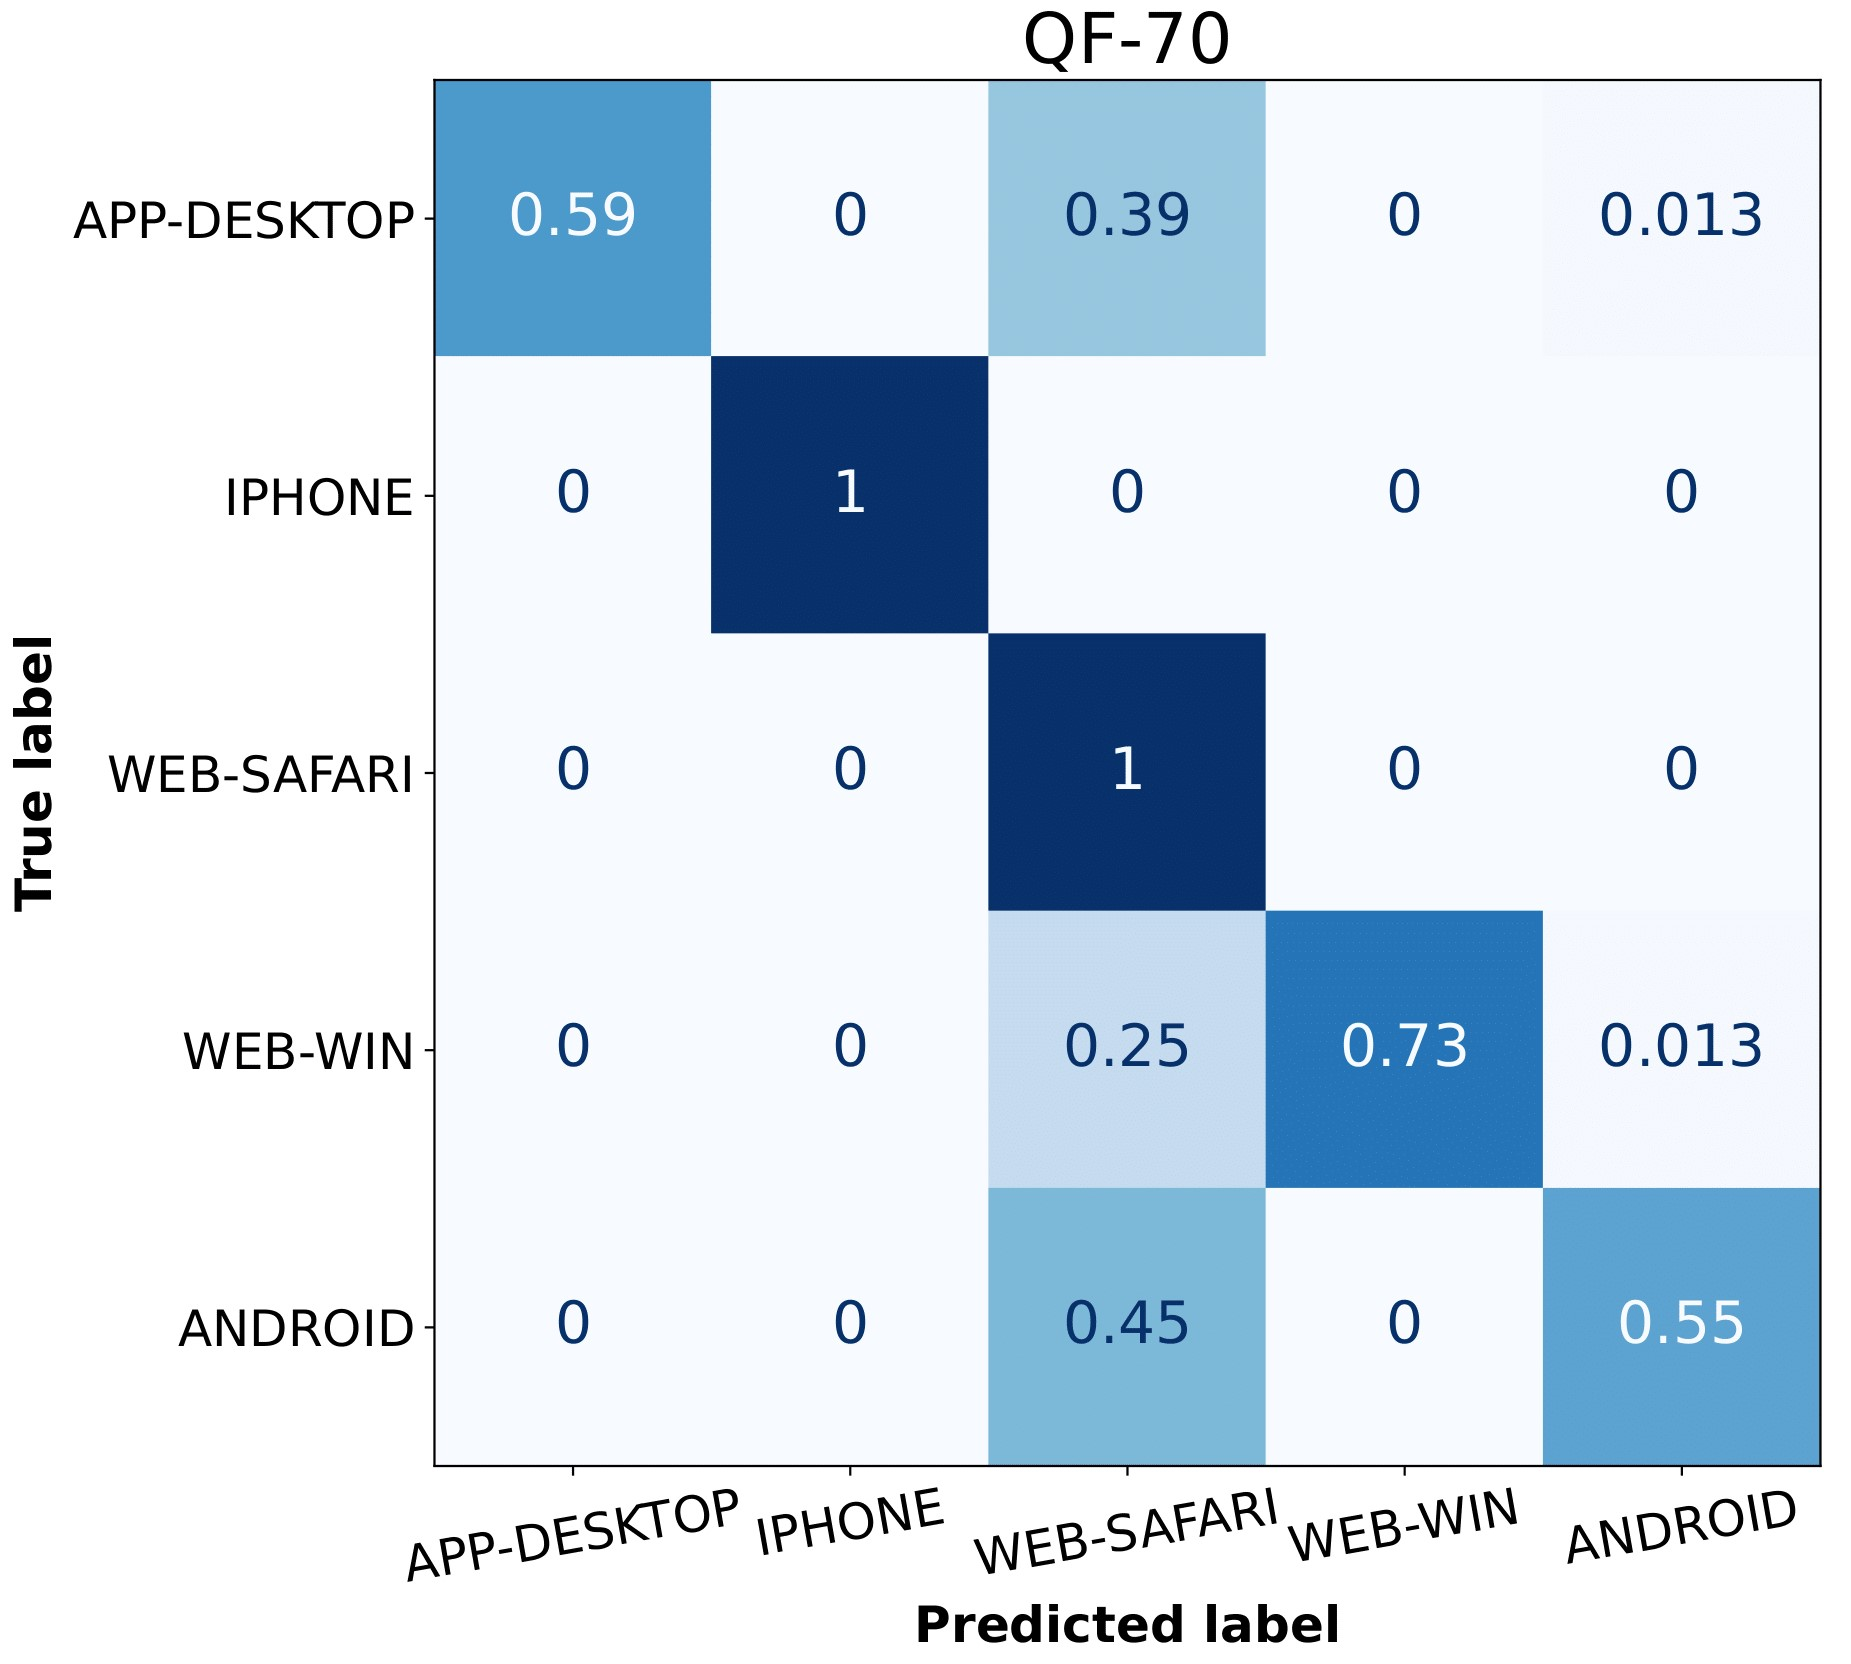
\includegraphics[width=8cm, height=8cm, keepaspectratio]{Immagini/Classificazione/confusion_matrix_SVM_QF-70.jpg}}\ \ \ \ \
%     \subfloat[][]{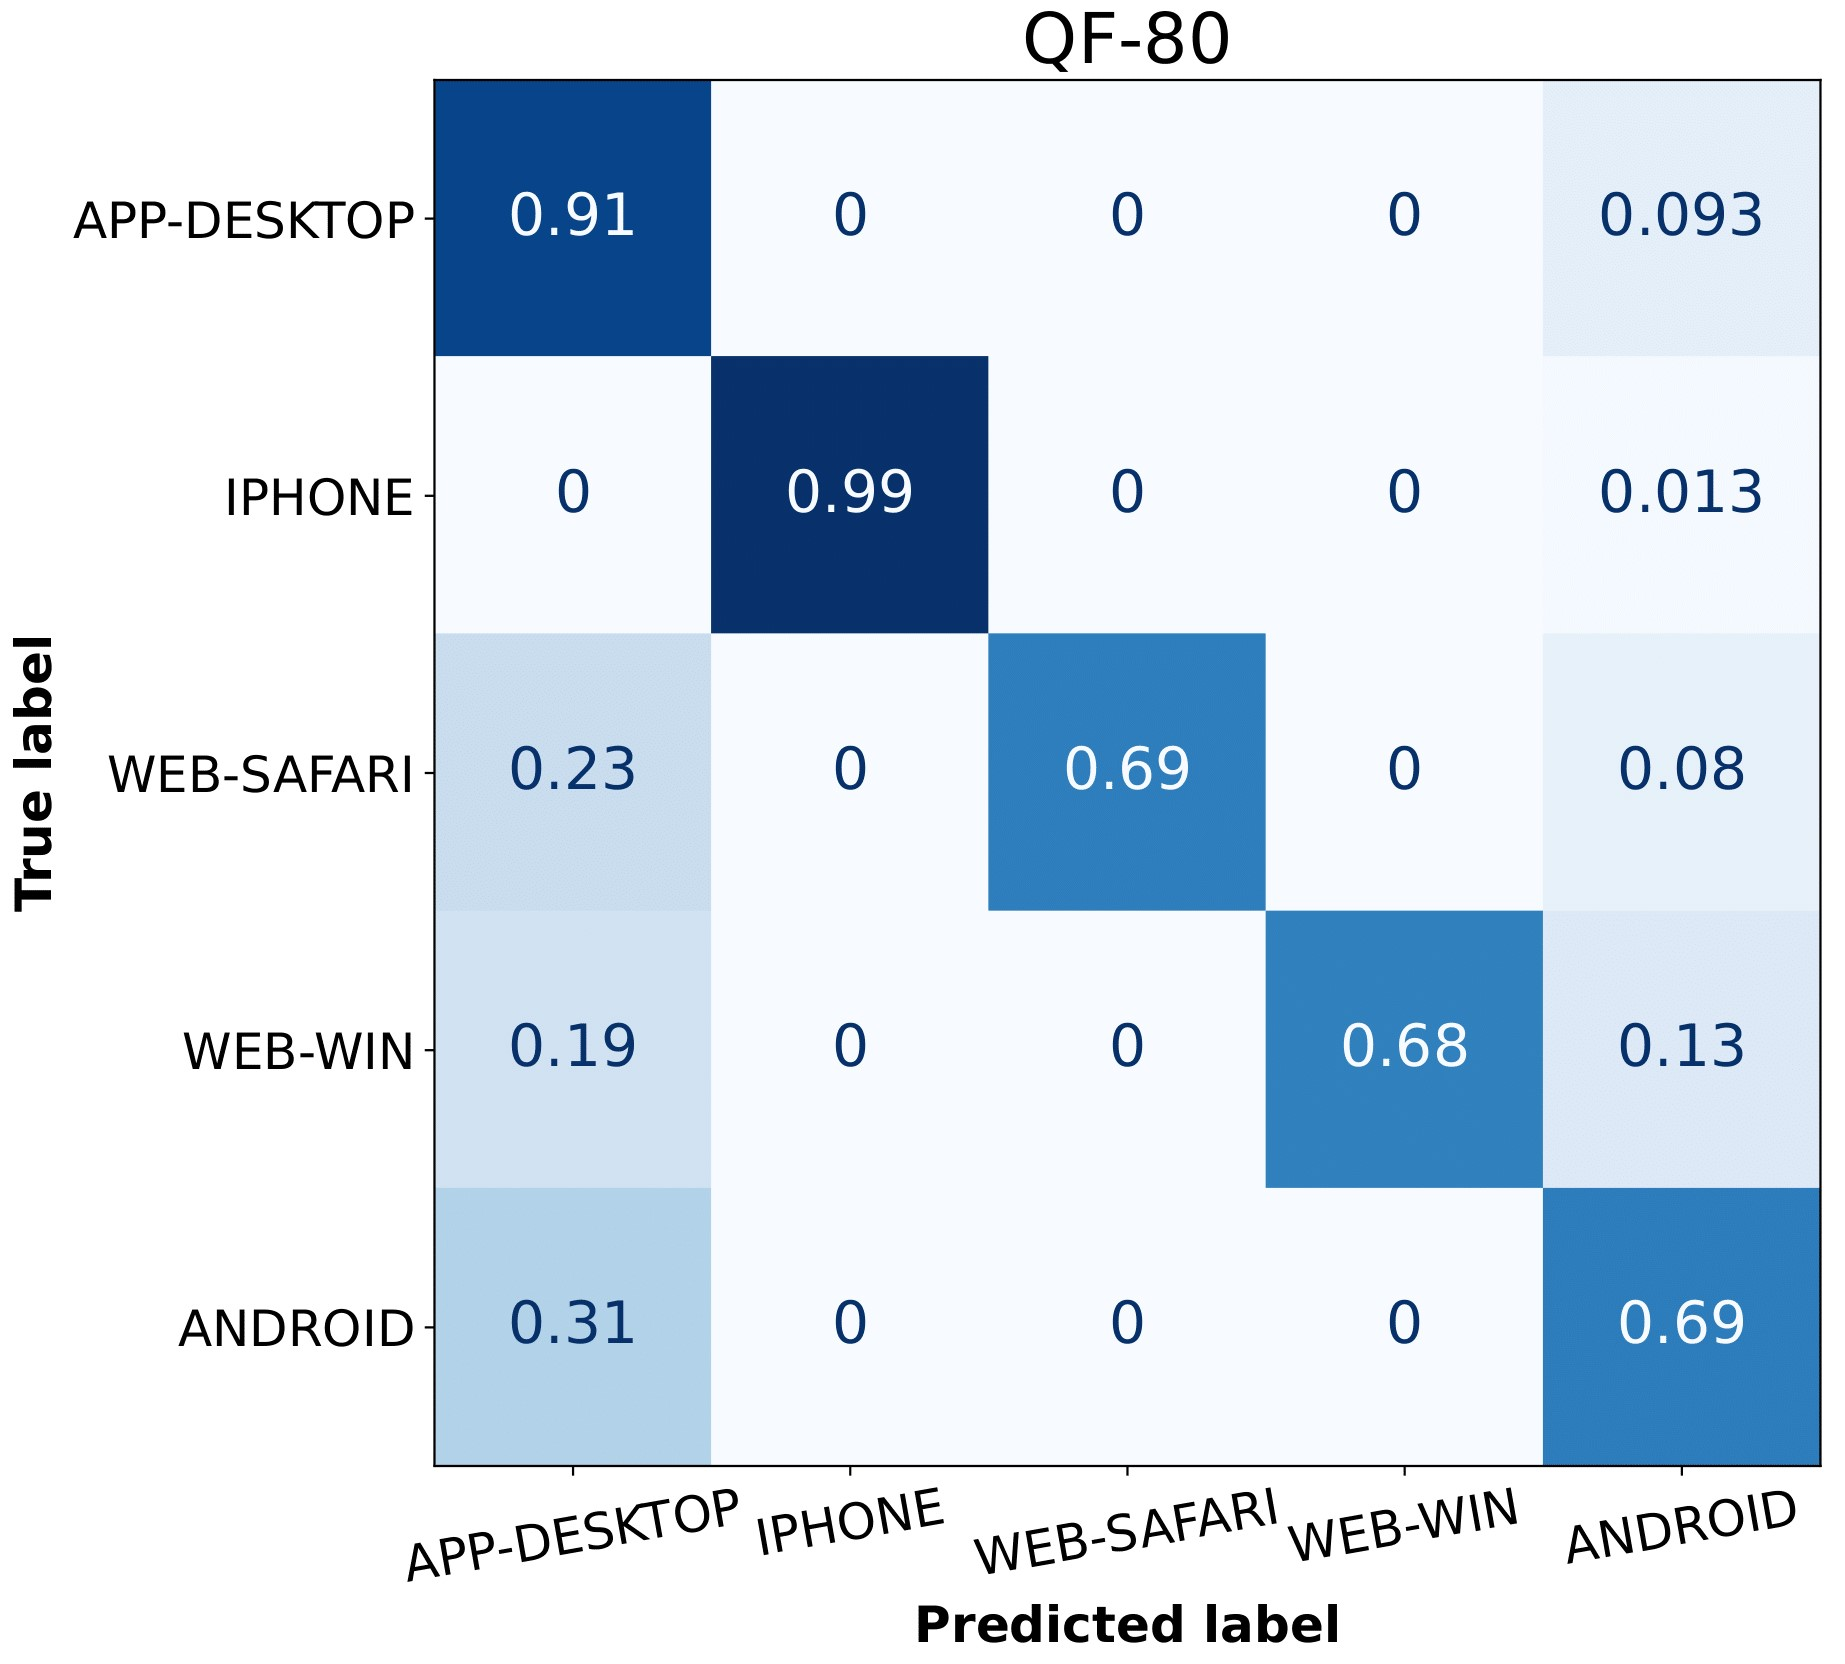
\includegraphics[width=8cm, height=8cm, keepaspectratio]{Immagini/Classificazione/confusion_matrix_SVM_QF-80.jpg}}\\
%     \subfloat[][]{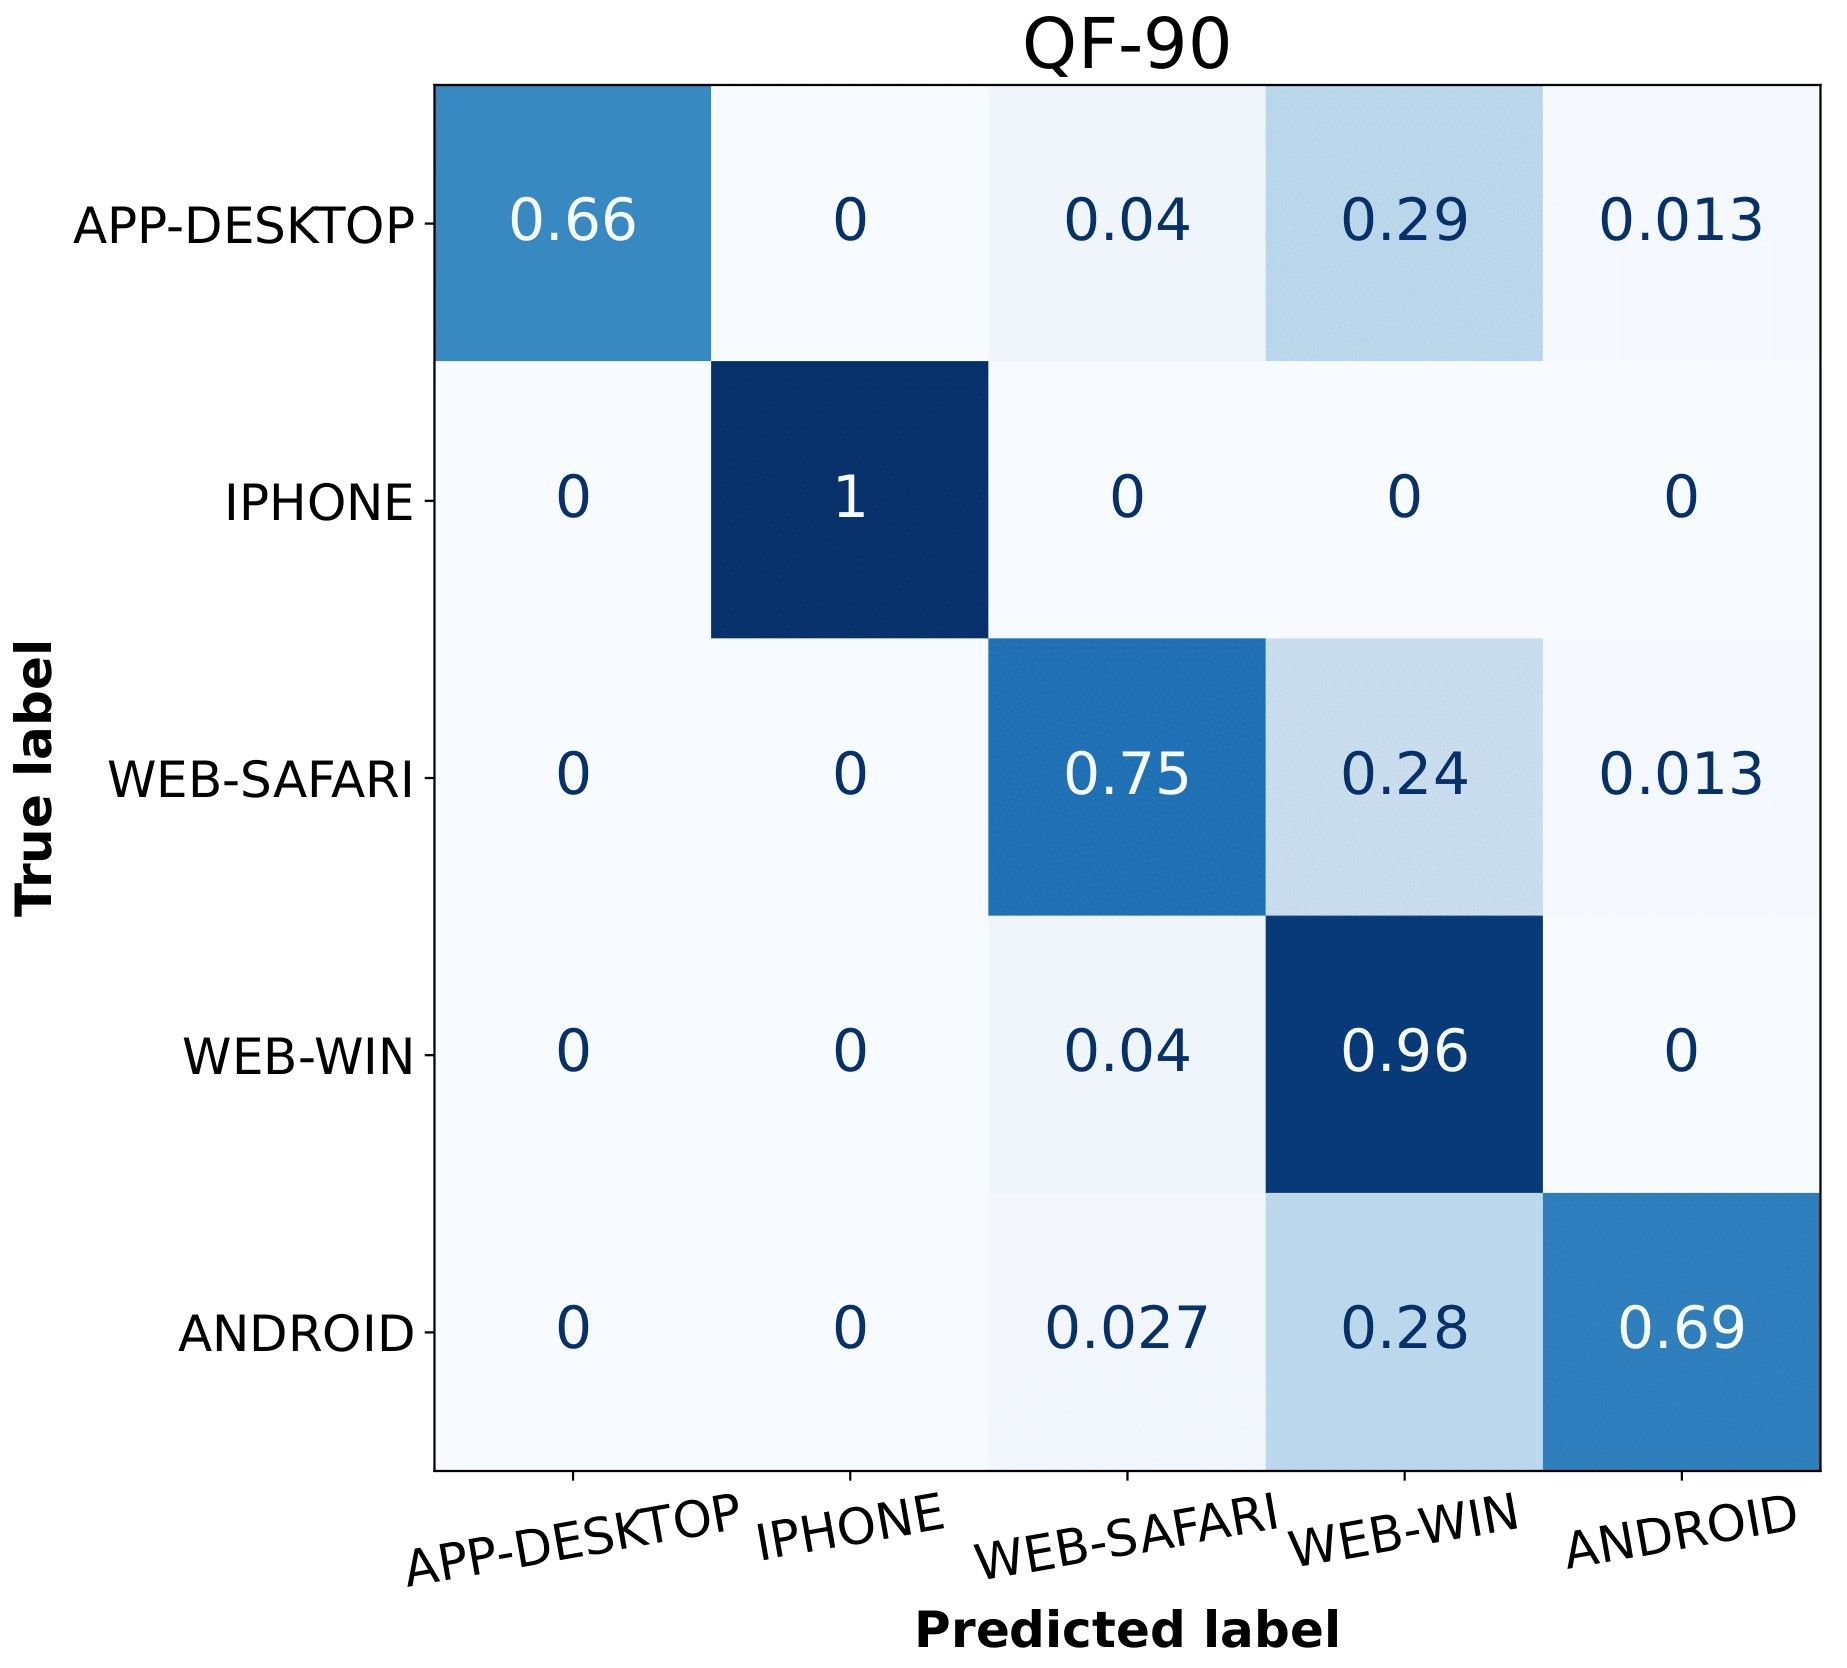
\includegraphics[width=8cm, height=8cm, keepaspectratio]{Immagini/Classificazione/confusion_matrix_SVM_QF-90.jpg}}\ \ \ \ \
%     \subfloat[][]{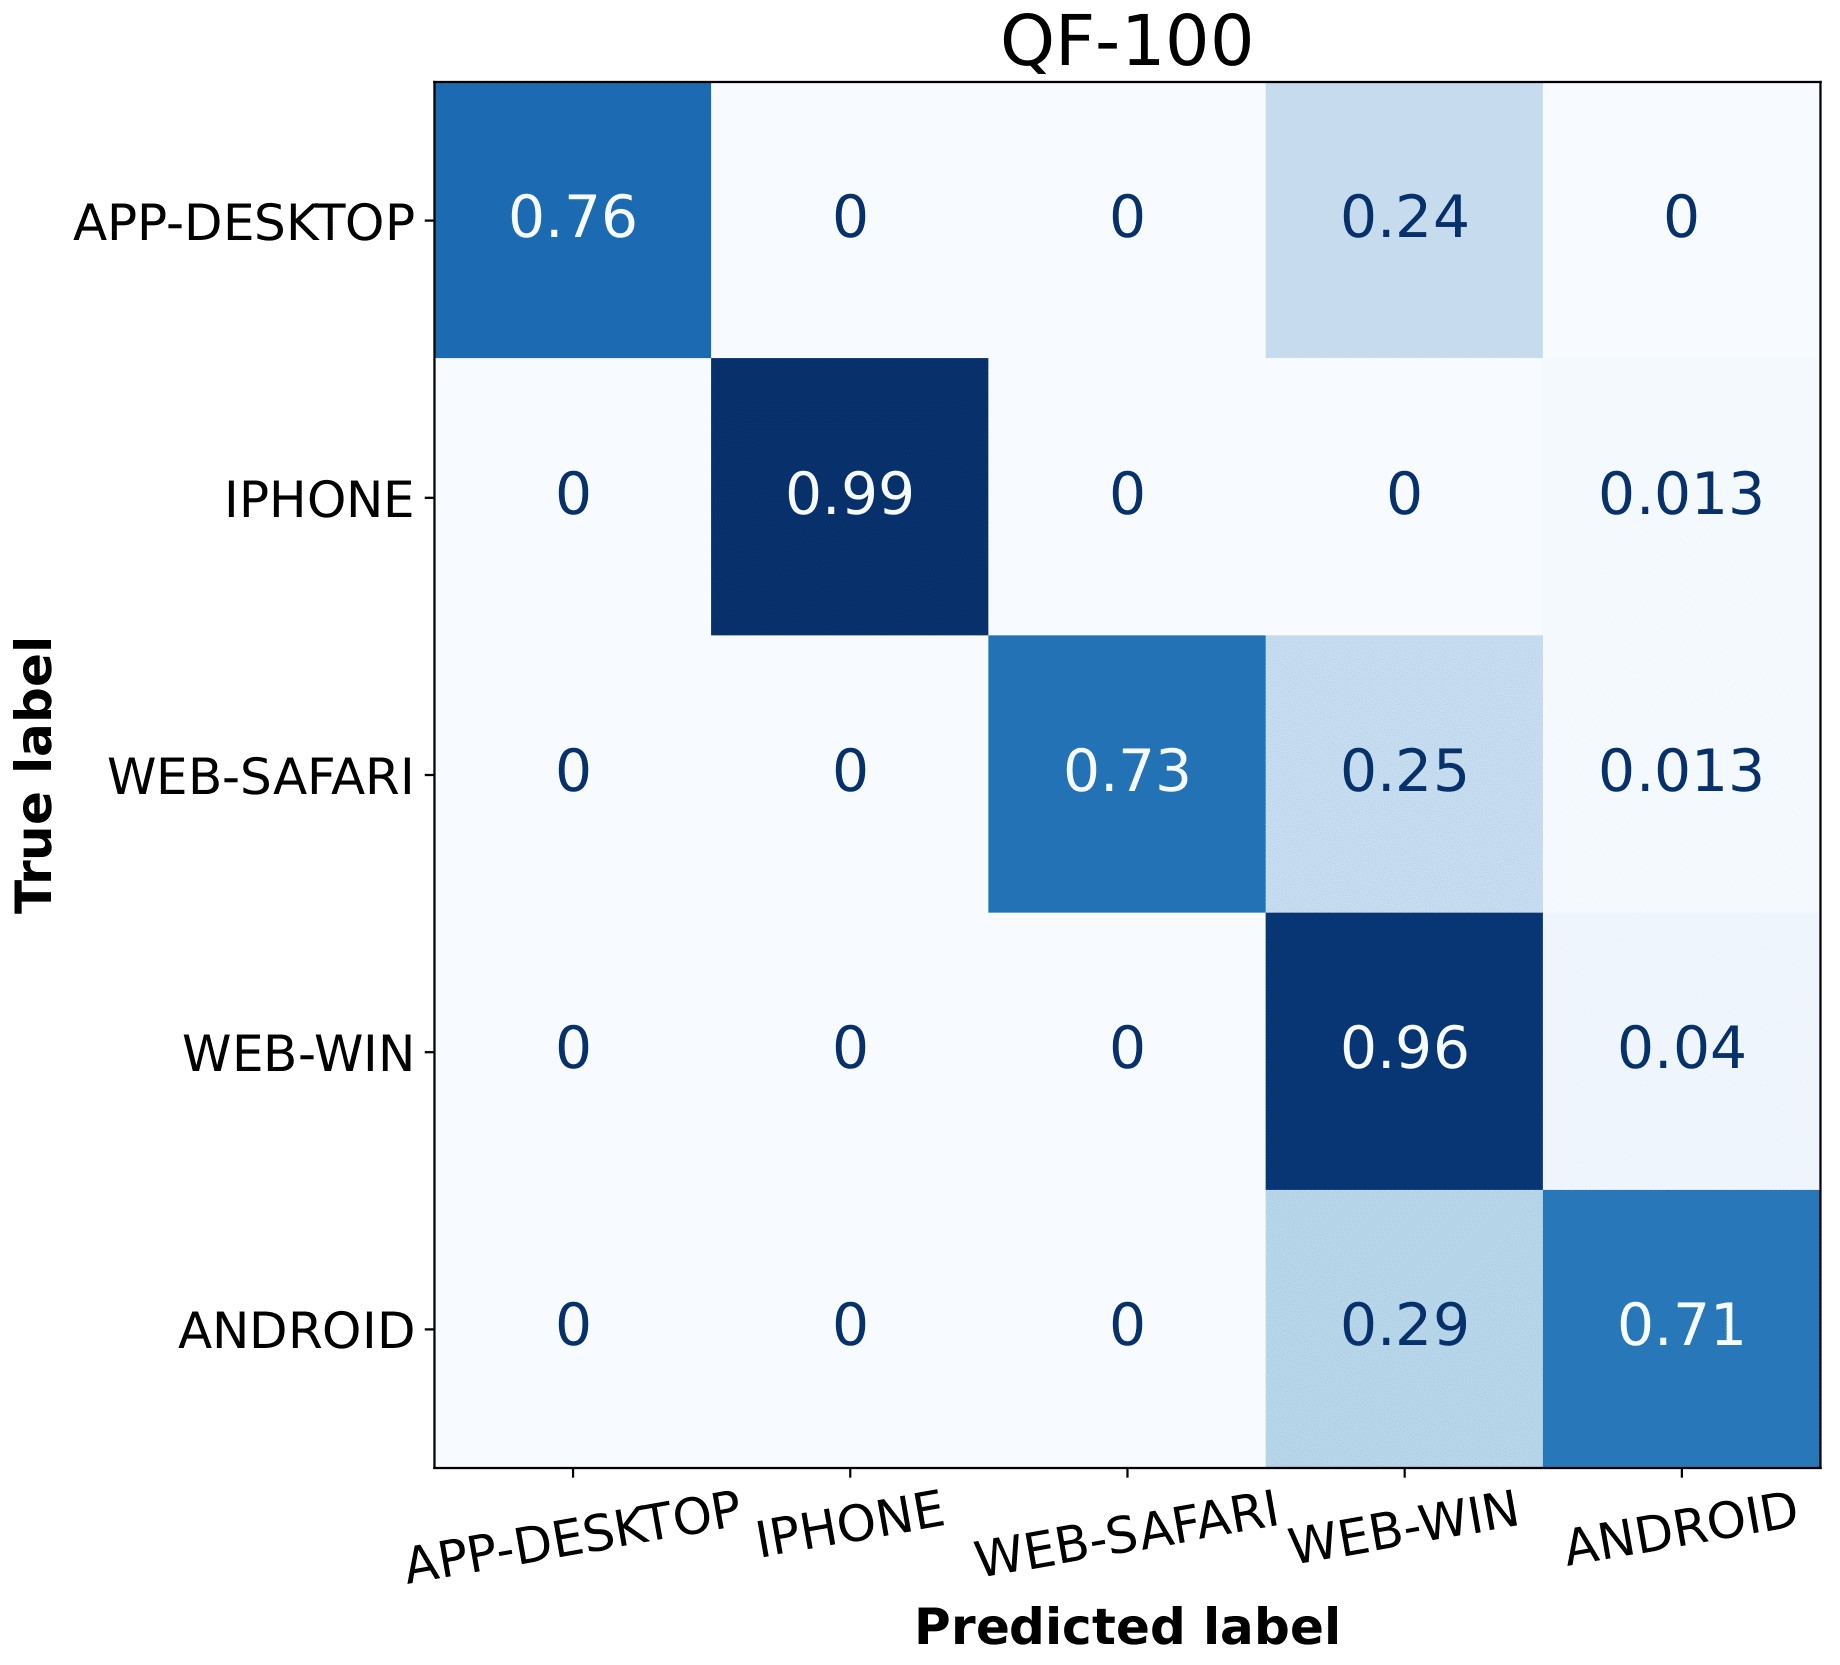
\includegraphics[width=8cm, height=8cm, keepaspectratio]{Immagini/Classificazione/confusion_matrix_SVM_QF-100.jpg}}
%     \caption{\textit{Confusion matrix} per \textit{support vector machine} divise per \textit{quality factor}.}
%     \label{fig:class_QF_SVM}
% \end{figure}

\vspace{1em}

Mettendo assieme tutti i risultati del calcolo del \textit{Mean Square Error} e del \textit{Peak Signal-to-Noise Ratio}, della visualizzazione Isomap e della classificazione possiamo dire di riuscire a distinguere qualora un'immagine provenga:

\begin{itemize}
    \item da un dispositivo mobile, distinguendo tra Apple e Android;
    \item da un'applicazione desktop;
    \item da un browser, distinguendo tra Safari e Chrome.
\end{itemize}


